\chapter{Synthetic Lethal Analysis of Gene Expression Data}
\label{chap:SLIPT}

Having developed a statistical \gls{synthetic lethal} detection methodology, \gls{SLIPT}, it was next applied to publicly available cancer \gls{gene expression} datasets. The analysis presented in this Chapter focuses on breast cancer for which  \gls{TCGA} \glslink{gene expression}{expression} data \citep{TCGA2012} from a patient cohort and \gls{siRNA} screen data, from experiments conducted in MCF10A cells \citep{Telford2015}, were available. Stomach cancer data \citep{TCGA2014GC} was used to replicate findings in an independent dataset, with this cancer chosen because it also occurs in syndromic \gls{HDGC} patients. The \gls{TCGA} data also has the advantages of having other clinical and molecular profiles, including \glslink{somatic}{somatic} \gls{mutation} across many of the same samples, in addition to a considerable sample size for \gls{RNA-Seq} \glslink{gene expression}{expression} data generated with common \gls{TCGA} procedures to minimise batch effects. %Some findings were replicated in the \gls{CCLE} \citep{Barretina2012} for comparison to the cell line experiments.

Synthetic lethal candidate partners for \textit{CDH1} were identified at both the gene and pathway level. \gls{SLIPT} gene candidates were analysed by cluster analysis for common \glslink{gene expression}{expression} profiles across samples and relationships with clinical factors and \glspl{mutation} in key breast cancer genes. These genes were also compared to the gene candidates from primary and secondary (validation) screens conducted by \citet{Telford2015} on isogenic cell lines. For comparison, the \gls{SLIPT} methodology was also applied using \gls{mutation} data for \textit{CDH1} against \glslink{gene expression}{expression} of candidate partners (as described in Section~\ref{methods:SLIPT}) which may better represent the null \glspl{mutation} in \gls{HDGC} patients and the experimental cell model \citep{Chen2014}. Pathways were analysed by over-representation analysis (with resampling for comparisons with \gls{siRNA} data) and supported by a \gls{metagene} analysis of pathway gene signatures. The pathway meta\gls{gene expression} profiles were used to replicate known relationships between clinical and molecular characteristics for breast cancer and to demonstrate application of \gls{SLIPT} directly on \glspl{metagene} to detect \gls{synthetic lethal} pathways.

\section{Synthetic Lethal Genes in Breast Cancer} \label{chapt3:exprSL_genes}

The \gls{SLIPT} methodology (as described in Section~\ref{methods:SLIPT}) was applied to the normalised \gls{TCGA} breast cancer \gls{gene expression} dataset ($n = 1168$). As shown in Table~\ref{tab:gene_SL}, the most significant genes had strong evidence of \glslink{gene expression}{expression}-based association with \textit{CDH1} (high $\chi^2$ values) with fewer samples exhibiting low \glslink{gene expression}{expression} of both genes than expected statistically. Eukaryotic translation genes were among the highest scoring gene candidates, including initiation factors, elongation factors, and ribosomal proteins. These are clearly necessary for cancer cells to grow and proliferate, with sustained \gls{gene expression} needed to maintain growth signalling pathways and resist apoptosis or immune factors, translation genes may be subject to \gls{non-oncogene addiction} for \textit{CDH1}-deficient cells.

While these are among the strongest \gls{synthetic lethal} candidates, translational genes are cruicial to the viability of healthy cells and dosing for a selective \gls{synthetic lethal} effect against these may be difficult compared to other biological functions which may also be supported among the \gls{SLIPT} candidate genes. Furthermore, few known biological functions of \textit{CDH1} were among the strongest SL candidates, so the remaining candidate genes may also be informative since they are likely to contain these expected functions in addition to novel relationships for \textit{CDH1}. Thus further pathway level analyses were also conducted to examine biological functions over-represent\-ed among synthetic candidate genes and to identify \gls{synthetic lethal} pathways.

\begin{table*}[!ht]
\caption{Candidate \gls{synthetic lethal} gene partners of \textit{CDH1} from SLIPT}
\label{tab:gene_SL}
\centering
\resizebox{0.8 \textwidth}{!}{
\begin{threeparttable}
\begin{tabular}{>{\em}sl^c^c^c^c^c}
\rowstyle{\bfseries}
 \em{Gene} & Observed\tnote{*}  & Expected\tnote{*} & $\chi^2$ value & p-value & p-value (\gls{FDR}) \\ 
  \hline
  \rowcolor{black!10}
TRIP10 & 62 & 130 & 162 & $5.65 \times 10^{-34}$ & $1.84 \times 10^{-31}$ \\
  \rowcolor{black!5} 
  EEF1B2 & 56 & 130 & 158 & $3.10 \times 10^{-33}$ & $9.45 \times 10^{-31}$ \\
  \rowcolor{black!10} 
  GBGT1 & 61 & 131 & 156 & $1.08 \times 10^{-32}$ & $3.14 \times 10^{-30}$ \\
  \rowcolor{black!5} 
  ELN & 81 & 130 & 149 & $3.46 \times 10^{-31}$ & $8.82 \times 10^{-29}$ \\
  \rowcolor{black!10} 
  TSPAN4 & 78 & 130 & 146 & $1.63 \times 10^{-30}$ & $3.79 \times 10^{-28}$ \\
  \rowcolor{black!5} 
  GLIPR2 & 72 & 130 & 146 & $1.68 \times 10^{-30}$ & $3.86 \times 10^{-28}$ \\
  \rowcolor{black!10} 
  RPS20 & 73 & 131 & 145 & $1.89 \times 10^{-30}$ & $4.28 \times 10^{-28}$ \\
  \rowcolor{black!5} 
  RPS27A & 80 & 130 & 143 & $5.53 \times 10^{-30}$ & $1.18 \times 10^{-27}$ \\
  \rowcolor{black!10} 
  EEF1A1P9 & 63 & 130 & 141 & $1.91 \times 10^{-29}$ & $3.74 \times 10^{-27}$ \\
  \rowcolor{black!5} 
  C1R & 73 & 130 & 141 & $2.05 \times 10^{-29}$ & $3.97 \times 10^{-27}$ \\
  \rowcolor{black!10} 
  LYL1 & 73 & 130 & 140 & $2.99 \times 10^{-29}$ & $5.74 \times 10^{-27}$ \\
  \rowcolor{black!5} 
  RPLP2 & 71 & 130 & 139 & $4.88 \times 10^{-29}$ & $9.07 \times 10^{-27}$ \\
  \rowcolor{black!10} 
  C10orf10 & 73 & 130 & 138 & $6.72 \times 10^{-29}$ & $1.20 \times 10^{-26}$ \\
  \rowcolor{black!5} 
  DULLARD & 74 & 131 & 138 & $9.29 \times 10^{-29}$ & $1.61 \times 10^{-26}$ \\
  \rowcolor{black!10} 
  PPM1F & 64 & 130 & 136 & $1.61 \times 10^{-28}$ & $2.65 \times 10^{-26}$ \\
  \rowcolor{black!5} 
  OBFC2A & 69 & 130 & 136 & $2.49 \times 10^{-28}$ & $3.93 \times 10^{-26}$ \\
  \rowcolor{black!10} 
  RPL11 & 70 & 130 & 136 & $2.56 \times 10^{-28}$ & $3.97 \times 10^{-26}$ \\
  \rowcolor{black!5} 
  RPL18A & 70 & 130 & 135 & $3.08 \times 10^{-28}$ & $4.70 \times 10^{-26}$ \\
  \rowcolor{black!10} 
  MFNG & 76 & 131 & 133 & $7.73 \times 10^{-28}$ & $1.12 \times 10^{-25}$ \\
  \rowcolor{black!5} 
  RPS17 & 77 & 131 & 133 & $8.94 \times 10^{-28}$ & $1.29 \times 10^{-25}$ \\
  \rowcolor{black!10} 
  MGAT1 & 73 & 130 & 132 & $1.44 \times 10^{-27}$ & $2.03 \times 10^{-25}$ \\
  \rowcolor{black!5} 
  RPS12 & 72 & 130 & 128 & $8.57 \times 10^{-27}$ & $1.12 \times 10^{-24}$ \\
  \rowcolor{black!10} 
  C10orf54 & 73 & 130 & 127 & $1.37 \times 10^{-26}$ & $1.75 \times 10^{-24}$ \\
  \rowcolor{black!5} 
  LOC286367 & 72 & 130 & 126 & $2.20 \times 10^{-26}$ & $2.70 \times 10^{-24}$ \\
  \rowcolor{black!10} 
  GMFG & 70 & 130 & 126 & $2.20 \times 10^{-26}$ & $2.70 \times 10^{-24}$ \\ 
  \hline
\end{tabular}
\begin{tablenotes}
\raggedright \small
Strongest candidate \gls{synthetic lethal} partners for \textit{CDH1} by \gls{SLIPT} in \gls{TCGA} breast cancer expression data

\item[*] Observed and expected numbers of samples which had low \glslink{gene expression}{expression} of both genes
\end{tablenotes}
\end{threeparttable}
}
\end{table*}

The modified \acrshort{mtSLIPT} methodology (as described in Section~\ref{methods:SLIPT}) was also applied to the normalised \gls{TCGA} breast cancer \gls{gene expression} dataset, against \glslink{somatic}{somatic} loss of function \glspl{mutation} in \textit{CDH1}. As shown in  Appendix Table~\ref{tab:gene_mtSL}, the most significant genes also had strong evidence of \glslink{gene expression}{expression} associated with \textit{CDH1} \glspl{mutation} (high $\chi^2$ values) with fewer samples with \textit{CDH1} exhibiting low \glslink{gene expression}{expression} each candidate gene than expected statistically. These genes were not as strongly supported as the \glslink{gene expression}{expression} analysis (in Table~\ref{tab:gene_SL}), however, nor were as many genes detected. This is perhaps unsurprising due to the lower sample size with matching \glslink{somatic}{somatic} \gls{mutation} data and the lower frequency of \textit{CDH1} \glspl{mutation} compared to low \glslink{gene expression}{expression} defined by $\sfrac{1}{3}$ quantiles.

The \acrshort{mtSLIPT} candidates had more genes involved in cell and gene regulation, particularly \acrshort{DNA} and \acrshort{RNA} binding factors. The strongest candidates also included microtubule (\textit{KIF12}), microfibril (\textit{MFAP4}), and cell adhesion (\textit{TENC1}) genes consistent with the established cytoskeletal role of \textit{CDH1}. The elastin gene (\textit{ELN}) was notably strongly supported by both \glslink{gene expression}{expression} and \gls{mutation} \gls{SLIPT} analysis of \text{CDH1} supporting interactions with extracellular proteins and the tumour microenvironment.

%%appendix
%\label{tab:gene_mtSL}

\subsection{Synthetic Lethal Pathways in Breast Cancer} \label{chapt3:exprSL_pathways}

Translational pathways were strongly over-represented in \gls{SLIPT} partners, as shown in Table~\ref{tab:pathway_exprSL}. These include ribosomal subunits, initiation, peptide elongation, and termination. Regulatory processes involving \acrshort{mRNA} including 3' untranslated region (UTR) binding, L13a-mediated translational silencing, and nonsense-mediated decay were also implicated. These are consistent with protein translation being subject to ``\gls{non-oncogene addiction}'' \citep{Luo2009}, as a core process that is dysregulated to sustain cancer proliferation and survival \citep{Gao2015}.

Immune pathways, including the adaptive immune system and responses to infectious diseases were also strongly implicated as \gls{synthetic lethal} with loss of \gls{E-cadherin}. This is consistent with the alterations of immune response being a hallmark of cancer \cite{Hanahan2000}, since evading the immune system is necessary for cancer survival. Either of these systems are potential means to target \textit{CDH1} deficient cells, although these were not detected in an isolated cell line experimental screen \citep{Telford2015} and the differences between the findings in patient data are described in more detail in Section~\ref{chapt3:compare_pathway}.

\begin{table*}[!ht]
\caption{Pathways for \textit{CDH1} partners from SLIPT}
\label{tab:pathway_exprSL}
\centering
\resizebox{1 \textwidth}{!}{
\begin{threeparttable}
\begin{tabular}{lccc}
  \cellcolor{white} \textbf{Pathways Over-represented} & \textbf{Pathway Size} & \textbf{SL Genes} & \textbf{p-value (\gls{FDR})} \\
  \hline
  \rowcolor{black!10}
  Eukaryotic Translation Elongation &  86 &  81 & $1.3 \times 10^{-207}$ \\ 
  \rowcolor{black!5}
  Peptide chain elongation &  83 &  78 & $5.6 \times 10^{-201}$ \\ 
  \rowcolor{black!10}
  Eukaryotic Translation Termination &  83 &  77 & $1.2 \times 10^{-196}$ \\ 
  \rowcolor{black!5}
  Viral \acrshort{mRNA} Translation &  81 &  76 & $1.2 \times 10^{-196}$ \\ 
  \rowcolor{black!10}
  Formation of a pool of free 40S subunits &  93 &  81 & $3.7 \times 10^{-194}$ \\ 
  \rowcolor{black!5}
  Nonsense Mediated Decay independent of the Exon Junction Complex &  88 &  77 & $5.3 \times 10^{-187}$ \\ 
  \rowcolor{black!10}
  L13a-mediated translational silencing of Ceruloplasmin \glslink{gene expression}{expression} & 103 &  82 & $9.6 \times 10^{-183}$ \\ 
  \rowcolor{black!5}
  3' -UTR-mediated translational regulation & 103 &  82 & $9.6 \times 10^{-183}$ \\ 
  \rowcolor{black!10}
  GTP hydrolysis and joining of the 60S ribosomal subunit & 104 &  82 & $1.9 \times 10^{-181}$ \\ 
  \rowcolor{black!5}
  Nonsense-Mediated Decay & 103 &  80 & $6.2 \times 10^{-176}$ \\ 
  \rowcolor{black!10}
  Nonsense Mediated Decay enhanced by the Exon Junction Complex & 103 &  80 & $6.2 \times 10^{-176}$ \\ 
  \rowcolor{black!5}
  Adaptive Immune System & 412 & 167 & $6.5 \times 10^{-174}$ \\ 
  \rowcolor{black!10}
  Eukaryotic Translation Initiation & 111 &  82 & $5.7 \times 10^{-173}$ \\ 
  \rowcolor{black!5}
  Cap-dependent Translation Initiation & 111 &  82 & $5.7 \times 10^{-173}$ \\ 
  \rowcolor{black!10}
  SRP-dependent cotranslational protein targeting to membrane & 104 &  79 & $2.0 \times 10^{-171}$ \\ 
  \rowcolor{black!5}
  Translation & 141 &  91 & $6.1 \times 10^{-170}$ \\ 
  \rowcolor{black!10}
  Infectious disease & 347 & 146 & $1.6 \times 10^{-166}$ \\ 
  \rowcolor{black!5}
  Influenza Infection & 117 &  81 & $1.9 \times 10^{-163}$ \\ 
  \rowcolor{black!10}
  Influenza Viral \acrshort{RNA} Transcription and Replication & 108 &  77 & $1.9 \times 10^{-160}$ \\ 
  \rowcolor{black!5}
  Influenza Life Cycle & 112 &  77 & $2.5 \times 10^{-156}$ \\ 
   \hline
\end{tabular}
\begin{tablenotes}
\raggedright \small
Gene set over-representation analysis (hypergeometric test) for Reactome pathways in \gls{SLIPT} partners for \textit{CDH1}.
\end{tablenotes}
\end{threeparttable}
}
\end{table*}

It is also notable that the pathways over-represented in \gls{SLIPT} candidate genes have strongly significant over-representation of Reactome pathways based on the hypergeometric test (as described in Section~\ref{methods:enrichment}). Even after adjusting stringently for multiple testing, biologically related pathways were supported together. These pathways are further supported by testing for \glspl{synthetic lethal} against \textit{CDH1} \glspl{mutation} (\acrshort{mtSLIPT}) with many of these pathways also among the most strongly supported in this analysis (shown in Appendix Table~\ref{tab:pathway_mtSL}). This \gls{mutation}-based analysis more closely represents the null \textit{CDH1} \glspl{mutation} in \gls{HDGC} \citep{Guilford1998} and the experimental MCF10A cell model \citep{Chen2014}. There was still support for translational and immune pathways not detected in the isolated experimental system.  \glspl{GPCR} also among the most strongly supported pathways, supporting the experimental findings of \citet{Telford2015} for these intracellular signalling pathways already being targeted for other diseases. 

%%appendix
%\label{tab:pathway_mtSL}

\FloatBarrier


\subsection{Expression Profiles of Synthetic Lethal Partners} \label{chapt3:exprSL_clusters}

Due to the sheer number of gene candidates, investigations proceeded into correlation structure and pathway over-represent\-ation. These analyses also examined \glslink{gene expression}{expression} patterns of \gls{synthetic lethal} gene candidates. This serves to explore the functional similarity of the \gls{synthetic lethal} partners of \textit{CDH1}, with the eventual aim to assess their utility as drug targets. As shown in Figure~\ref{fig:slipt_expr} (which clusters \textit{CDH1} lowly expressing samples separately), there were several large clusters of genes among the  \glslink{gene expression}{expression} profiles of the \textit{CDH1} \gls{synthetic lethal} candidate partners. The clustering suggests co-regulation of genes or pathway correlation between partner gene candidates. A number of candidates from an experimental \gls{RNAi} screen study performed by \citet{Telford2015} were also identified by this approach. In addition, novel gene candidates were also identified, which had not been observed affect viability in isogenic cell line experiments. %or in some cases, even opposite effects of selective cell death or toxicity to both isogenic cell lines.

\begin{figure*}[!htbp]
%\begin{mdframed}
  \centering
  \resizebox{0.99 \textwidth}{!}{
    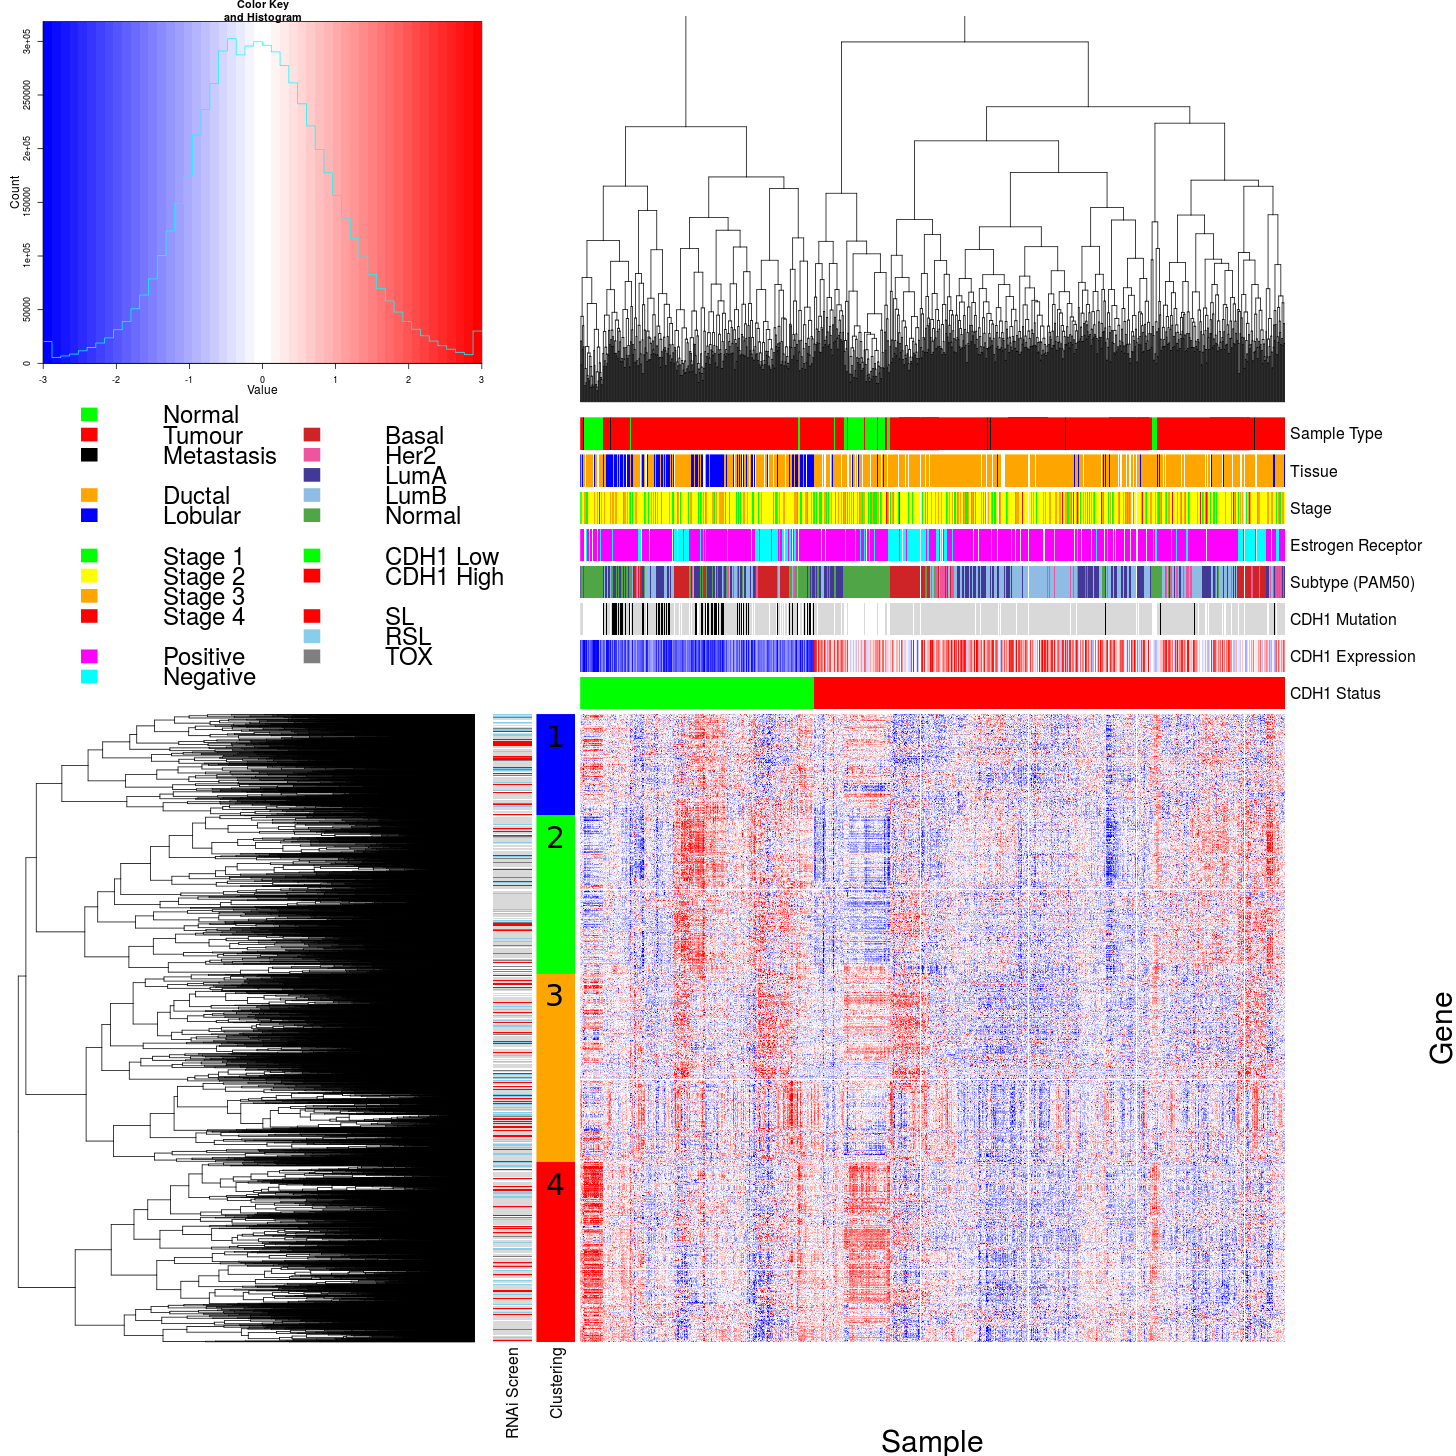
\includegraphics{CDH1_Heatmaps_Genes_Split_By_CDH1_z-trans_exprSL_cordistx_Pub.png}
   }
    \caption[Synthetic lethal \glslink{gene expression}{expression} profiles of analysed samples]{\small \textbf{Synthetic lethal \glslink{gene expression}{expression} profiles of analysed samples.} \Gls{gene expression} profile heatmap (correlation distance, complete linkage) of all samples (separated by the $\sfrac{1}{3}$ quantile of \textit{CDH1} \glslink{gene expression}{expression}) analysed in \gls{TCGA} breast cancer dataset for \gls{gene expression} of 5165 candidate partners of \gls{E-cadherin} (\textit{CDH1}) from \gls{SLIPT} prediction (with \gls{FDR} adjusted $p < 0.05$). Deeply clustered, inter-correlated genes form several main groups, each containing genes that were SL candidates or lethal in an \gls{siRNA} screen \citep{Telford2015}. Screen results for \gls{synthetic lethal} (SL), the reverse effect (RSL), or lethal cell viability are shown as reported by \citet{Telford2015}. Clusters had different sample groups highly expressing the \gls{synthetic lethal} candidates in \textit{CDH1} low samples, notably `normal-like', `basal-like', and estrogen receptor negative samples have elevated \glslink{gene expression}{expression} in one or more distinct clusters showing complexity and variation among candidate \gls{synthetic lethal} partners. \textit{CDH1} low samples also contained most of samples with \textit{CDH1} \glspl{mutation} (shown in black). Negative values for \gls{mutation} and screen data are shown in light grey, with missing data in white.
   %This suggests that multiple targets may be needed to target \textit{CDH1} deficiency across genetic backgrounds and that combination therapy may be more effective. 
}
\label{fig:slipt_expr}
%\end{mdframed}
\end{figure*}

In these \glslink{gene expression}{expression} profiles, a gene with a moderate or high signal across samples exhibiting low \textit{CDH1} \glslink{gene expression}{expression} would represent a potential drug target. However, it appears that several molecular subtypes of cancer have elevation of different clusters of \gls{synthetic lethal} candidates in samples with low \textit{CDH1}. This clustering suggests that different targets (or combinations) could be effective in different patients, suggesting potential utility for stratification.  In particular, estrogen receptor negative, basal-like subtype, and ``normal-like'' tumours \citep{Eroles2012, Parker2009, Dai2015} have elevation of genes specific to particular clusters, indicative of some \gls{synthetic lethal} interactions being specific to a particular molecular subtype or genetic background. Thus \gls{synthetic lethal} drug therapy against these subtypes may be ineffective if it were designed against genes in another cluster.
 
A similar correlation structure was observed among the candidates tested against \textit{CDH1} \gls{mutation} (\acrshort{mtSLIPT}), as shown in Appendix Figure~\ref{fig:slipt_expr_mtSL}. This clustering analysis similarly identified several major clusters of putative \gls{synthetic lethal} partner genes. In this case, many partner genes had consistently high \glslink{gene expression}{expression} across most of the (predominantly lobular subtype) \textit{CDH1} breast cancer samples. However, a major exception to this in the \textit{CDH1} \glslink{gene expression}{expression} analysis were the normal tissue samples which were excluded from the \gls{mutation} data (as they were not tested for tumour-specific genotypes). This supports \gls{synthetic lethal} interventions being more applicable to \textit{CDH1} \gls{mutant} tumours. There was still considerable correlation structure, particularly among \textit{CDH1}\gls{wild-type} samples, sufficient to distinguish gene clusters. In contrast to the \glslink{gene expression}{expression} analysis the (predominantly ductal \textit{CDH1}\gls{wild-type}) basal-like subtype and estrogen receptor negative samples had depleted \glslink{gene expression}{expression} among most candidate \gls{synthetic lethal} partners. This is consistent with \gls{synthetic lethal} interventions only being effective in lobular estrogen receptor positive breast cancers in which they are a more common, as recurrent (\glslink{driver mutation}{driver}) \gls{mutation}. However, the remaining samples are still informative for \gls{synthetic lethal} analysis (by \gls{SLIPT}) as it requires highly expressing \textit{CDH1} samples for comparison.

%\FloatBarrier

The \textit{CDH1} \gls{mutant} samples (in Figure~\ref{fig:slipt_expr}) were predominantly among the low \textit{CDH1} expressing samples, clustering throughout them with similar expression profiles to other samples exhibiting low \textit{CDH1} expression. Thus the molecular profiles of \textit{CDH1} low samples were indistinguishable from \textit{CDH1} \gls{mutant} samples, with the exception of normal samples (that do not have \glslink{somatic}{somatic} \gls{mutation} data available). Conversely, many of the \textit{CDH1} \gls{mutant} samples (in Appendix Figure~\ref{fig:slipt_expr_mtSL}) had among the lowest \textit{CDH1} \glslink{gene expression}{expression}, and some of the \gls{synthetic lethal} partners were also highly expressed in low expressing \textit{CDH1}\gls{wild-type} samples, despite these not being considered as ``inactivated'' by \acrshort{mtSLIPT} analysis.

Together these results support the use of low \textit{CDH1} \glslink{gene expression}{expression} as a strategy for detecting \textit{CDH1} inactivation. This has the benefit of increasing sample size (including samples such as normal tissue which do not have \glslink{somatic}{somatic} \gls{mutation} data available) and increasing the expected number of mutually inactive (low-low) samples for the directional criteria of (mt)\gls{SLIPT} which enables it to better distinguish significant deviations below this (as discussed in Section~\ref{chapt5:compare_methods}). This also circumvents the assumption that all (detected) \glspl{mutation} are inactivating (although synonymous \glspl{mutation} were excluded from the analysis), which may not be the case for several highly expressing \textit{CDH1} \gls{mutant} samples that do not cluster together in Figure~\ref{fig:slipt_expr} or Appendix Figure~\ref{fig:slipt_expr_mtSL}. One of these exhibits among the lowest \glslink{gene expression}{expression} for many predicted \gls{synthetic lethal} partners and would not be vulnerable to inactivation of these genes. As such, correctly genotyping inactivating \glspl{mutation} will be \gls{essential} in clinical practice for \gls{synthetic lethal} targeting of \gls{tumour suppressor} genes, particularly for other genes such as \textit{TP53} where oncogenic and \gls{tumour suppressor} \glspl{mutation} (with different molecular consequences) are both commons. Using \glslink{gene expression}{expression} as a measure of gene function also avoids the assumptions that \glspl{mutation} are \glslink{somatic}{somatic}, rather than \gls{germline}, and that gene inactivation occurs by detectable \glspl{mutation}, rather than other mechanisms such as epigenetic changes. These may also account for some of the lowly expressing \textit{CDH1}\gls{wild-type} samples clustering with similar profiles to \gls{mutant} samples.

%%appendix
%\label{fig:slipt_expr_mtSL}

%Figure 3.   Heatmap of \gls{RNA-Seq} \gls{gene expression} in predicted SL partners of \textit{CDH1} showing distinct subgroups of SL partners and \glslink{edge}{links} between SL partner \glslink{gene expression}{expression} and clinical variables.

\FloatBarrier

\subsubsection{Subgroup Pathway Analysis}

%Table 5.  Gene set enrichment results for subgroups of \textit{CDH1} SL partners shows functional variation.


\begin{table*}[!hp]
\caption{Pathways for clusters of \textit{CDH1} partners from SLIPT}
\label{tab:pathway_clusters}
\centering
%\begin{tiny}
%\makebox[\textwidth][c]{
\resizebox{0.75 \textwidth}{!}{
\begin{threeparttable}
\begin{tabular}{lccc}
%\caption{Pathway composition for clusters of \textit{CDH1} partners from SLIPT}
%\label{tab:pathway_clusters}
  \large{\textbf{Pathways Over-represented in Cluster 1}} & \large{\textbf{Pathway Size}} & \large{\textbf{Cluster Genes}} & \large{\textbf{p-value (\gls{FDR})}} \\ %(833 genes)  
  \hline
  \rowcolor{Cluster_Blue!20}
  Collagen formation &  67 &  10 & $4.0 \times 10^{-11}$ \\
  \rowcolor{Cluster_Blue!15} 
  Extracellular matrix organisation & 238 &  21 & $1.8 \times 10^{-9}$ \\
  \rowcolor{Cluster_Blue!20} 
  Collagen biosynthesis and modifying enzymes &  56 &   8 & $1.8 \times 10^{-9}$ \\
  \rowcolor{Cluster_Blue!15} 
  Uptake and actions of bacterial toxins &  22 &   5 & $9.5 \times 10^{-9}$ \\
  \rowcolor{Cluster_Blue!20} 
  Elastic fibre formation &  37 &   6 & $1.9 \times 10^{-8}$ \\
  \rowcolor{Cluster_Blue!15} 
  Muscle contraction &  62 &   7 & $2.4 \times 10^{-7}$ \\
  \rowcolor{Cluster_Blue!20} 
  Fatty acid, triacylglycerol, and ketone body metabolism & 117 &  10 & $4.9 \times 10^{-7}$ \\
  \rowcolor{Cluster_Blue!15} 
  XBP1(S) activates chaperone genes &  51 &   6 & $6.6 \times 10^{-7}$ \\
  \rowcolor{Cluster_Blue!20} 
  IRE1alpha activates chaperones &  54 &   6 & $1.2 \times 10^{-6}$ \\
  \rowcolor{Cluster_Blue!15} 
  Neurotoxicity of clostridium toxins &  10 &   3 & $1.3 \times 10^{-6}$ \\
  \rowcolor{Cluster_Blue!20} 
  Retrograde neurotrophin signalling &  10 &   3 & $1.3 \times 10^{-6}$ \\
  \rowcolor{Cluster_Blue!15} 
  Assembly of collagen fibrils and other multimeric structures &  40 &   5 & $1.9 \times 10^{-6}$ \\
  \rowcolor{Cluster_Blue!20} 
  Collagen degradation &  58 &   6 & $2.0 \times 10^{-6}$ \\
  \rowcolor{Cluster_Blue!15} 
  Arachidonic acid metabolism &  41 &   5 & $2.1 \times 10^{-6}$ \\
  \rowcolor{Cluster_Blue!20} 
  Synthesis of PA &  26 &   4 & $3.0 \times 10^{-6}$ \\
  \rowcolor{Cluster_Blue!15} 
  Signalling by NOTCH &  80 &   7 & $3.3 \times 10^{-6}$ \\
  \rowcolor{Cluster_Blue!20} 
  Signalling to RAS &  27 &   4 & $3.7 \times 10^{-6}$ \\
  \rowcolor{Cluster_Blue!15} 
  Integrin cell surface interactions &  82 &   7 & $4.2 \times 10^{-6}$ \\
%  \rowcolor{Cluster_Blue!20} 
%  Smooth Muscle Contraction &  28 &   4 & $4.4 \times 10^{-6}$ \\
%  \rowcolor{Cluster_Blue!15} 
%  ECM proteoglycans &  66 &   6 & $6.3 \times 10^{-6}$ \\ 
  \hline
  %\\
  \cellcolor{white} \large{\textbf{Pathways Over-represented in Cluster 2}} & \large{\textbf{Pathway Size}} & \large{\textbf{Cluster Genes}} & \large{\textbf{p-value (\gls{FDR})}} \\ %(833 genes)  
  \hline
  \rowcolor{Cluster_Green!20}
  Eukaryotic Translation Elongation &  86 &  75 & $1.1 \times 10^{-181}$ \\
  \rowcolor{Cluster_Green!15} 
  Viral \acrshort{mRNA} Translation &  81 &  72 & $9.8 \times 10^{-179}$ \\
  \rowcolor{Cluster_Green!20} 
  Peptide chain elongation &  83 &  72 & $1.9 \times 10^{-175}$ \\
  \rowcolor{Cluster_Green!15} 
  Eukaryotic Translation Termination &  83 &  72 & $1.9 \times 10^{-175}$ \\
  \rowcolor{Cluster_Green!20} 
  Formation of a pool of free 40S subunits &  93 &  75 & $1.9 \times 10^{-171}$ \\
  \rowcolor{Cluster_Green!15} 
  Nonsense Mediated Decay independent of the Exon Junction Complex &  88 &  72 & $9.9 \times 10^{-168}$ \\
  \rowcolor{Cluster_Green!20} 
  L13a-mediated translational silencing of Ceruloplasmin \glslink{gene expression}{expression} & 103 &  75 & $3.0 \times 10^{-159}$ \\
  \rowcolor{Cluster_Green!15} 
  3' -UTR-mediated translational regulation & 103 &  75 & $3.0 \times 10^{-159}$ \\
  \rowcolor{Cluster_Green!20} 
  Nonsense-Mediated Decay & 103 &  75 & $3.0 \times 10^{-159}$ \\
  \rowcolor{Cluster_Green!15} 
  Nonsense Mediated Decay enhanced by the Exon Junction Complex & 103 &  75 & $3.0 \times 10^{-159}$ \\
  \rowcolor{Cluster_Green!20} 
  SRP-dependent cotranslational protein targeting to membrane & 104 &  75 & $3.2 \times 10^{-158}$ \\
  \rowcolor{Cluster_Green!15} 
  GTP hydrolysis and joining of the 60S ribosomal subunit & 104 &  75 & $3.2 \times 10^{-158}$ \\
  \rowcolor{Cluster_Green!20} 
  Eukaryotic Translation Initiation & 111 &  75 & $4.5 \times 10^{-151}$ \\
  \rowcolor{Cluster_Green!15} 
  Cap-dependent Translation Initiation & 111 &  75 & $4.5 \times 10^{-151}$ \\
  \rowcolor{Cluster_Green!20} 
  Influenza Infection & 117 &  75 & $1.4 \times 10^{-145}$ \\
  \rowcolor{Cluster_Green!15} 
  Influenza Viral \acrshort{RNA} Transcription and Replication & 108 &  72 & $5.7 \times 10^{-145}$ \\
  \rowcolor{Cluster_Green!20} 
  Translation & 141 &  81 & $8.0 \times 10^{-143}$ \\
  \rowcolor{Cluster_Green!15} 
  Influenza Life Cycle & 112 &  72 & $2.3 \times 10^{-141}$ \\
%  \rowcolor{Cluster_Green!20} 
%  Infectious disease & 347 & 103 & $2.2 \times 10^{-95}$ \\
%  \rowcolor{Cluster_Green!15} 
%  Formation of the ternary complex, and subsequently, the 43S complex &  47 &  33 & $6.8 \times 10^{-80}$ \\
  \hline
  %\\
  \cellcolor{white} \large{\textbf{Pathways Over-represented in Cluster 3}} & \large{\textbf{Pathway Size}} & \large{\textbf{Cluster Genes}} & \large{\textbf{p-value (\gls{FDR})}} \\ %(833 genes)  
  \hline
  \rowcolor{Cluster_Orange!30}
  Adaptive Immune System & 412 &  90 & $6.1 \times 10^{-61}$ \\
  \rowcolor{Cluster_Orange!20} 
  Chemokine receptors bind chemokines &  52 &  27 & $6.7 \times 10^{-56}$ \\
  \rowcolor{Cluster_Orange!30} 
  Generation of second messenger molecules &  29 &  21 & $6.5 \times 10^{-55}$ \\
  \rowcolor{Cluster_Orange!20} 
  Immunoregulatory interactions between a Lymphoid and a non-Lymphoid cell &  64 &  29 & $6.5 \times 10^{-55}$ \\
  \rowcolor{Cluster_Orange!30} 
  TCR signalling &  62 &  27 & $8.9 \times 10^{-51}$ \\
  \rowcolor{Cluster_Orange!20} 
  Peptide ligand-binding receptors & 161 &  40 & $1.5 \times 10^{-45}$ \\
  \rowcolor{Cluster_Orange!30} 
  Translocation of ZAP-70 to Immunological synapse &  16 &  14 & $3.1 \times 10^{-43}$ \\
  \rowcolor{Cluster_Orange!20} 
  Costimulation by the CD28 family &  51 &  22 & $4.0 \times 10^{-43}$ \\
  \rowcolor{Cluster_Orange!30} 
  PD-1 signalling &  21 &  15 & $4.0 \times 10^{-41}$ \\
  \rowcolor{Cluster_Orange!20} 
  Class A/1 (Rhodopsin-like receptors) & 258 &  50 & $6.7 \times 10^{-41}$ \\
  \rowcolor{Cluster_Orange!30} 
  Phosphorylation of CD3 and TCR zeta chains &  18 &  14 & $1.3 \times 10^{-40}$ \\
  \rowcolor{Cluster_Orange!20} 
  Interferon gamma signalling &  74 &  24 & $5.0 \times 10^{-39}$ \\
  \rowcolor{Cluster_Orange!30} 
  GPCR ligand binding & 326 &  57 & $1.8 \times 10^{-38}$ \\
  \rowcolor{Cluster_Orange!20} 
  Cytokine Signalling in Immune system & 268 &  48 & $8.9 \times 10^{-37}$ \\
  \rowcolor{Cluster_Orange!30} 
  Downstream TCR signalling &  45 &  18 & $1.8 \times 10^{-35}$ \\
  \rowcolor{Cluster_Orange!20} 
  G$_{\alpha i}$ signalling events & 167 &  33 & $2.2 \times 10^{-33}$ \\
  \rowcolor{Cluster_Orange!30} 
  Cell surface interactions at the vascular wall &  99 &  21 & $1.3 \times 10^{-26}$ \\
  \rowcolor{Cluster_Orange!20} 
  Interferon Signalling & 164 &  28 & $1.7 \times 10^{-26}$ \\
%  \rowcolor{Cluster_Orange!30} 
%  Extracellular matrix organisation & 238 &  35 & $2.7 \times 10^{-25}$ \\
%  \rowcolor{Cluster_Orange!20} 
%  Antigen activates B Cell Receptor leading to generation of second messengers &  32 &  12 & $7.2 \times 10^{-25}$ \\
   \hline
  %\\ 
  \cellcolor{white} \large{\textbf{Pathways Over-represented in Cluster 4}} & \large{\textbf{Pathway Size}} & \large{\textbf{Cluster Genes}} & \large{\textbf{p-value (\gls{FDR})}} \\ %(833 genes)  
  \hline 
  \rowcolor{Cluster_Red!20}
  Extracellular matrix organisation & 238 &  48 & $8.0 \times 10^{-41}$ \\
  \rowcolor{Cluster_Red!15} 
  Class A/1 (Rhodopsin-like receptors) & 258 &  47 & $2.8 \times 10^{-36}$ \\
  \rowcolor{Cluster_Red!20} 
  GPCR ligand binding & 326 &  54 & $2.1 \times 10^{-34}$ \\
  \rowcolor{Cluster_Red!15} 
  G$_{\alpha s}$ signalling events &  83 &  22 & $1.4 \times 10^{-31}$ \\
  \rowcolor{Cluster_Red!20} 
  GPCR downstream signalling & 472 &  68 & $1.1 \times 10^{-29}$ \\
  \rowcolor{Cluster_Red!15} 
  Haemostasis & 423 &  61 & $3.3 \times 10^{-29}$ \\
  \rowcolor{Cluster_Red!20} 
  Platelet activation, signalling and aggregation & 180 &  31 & $7.1 \times 10^{-28}$ \\
  \rowcolor{Cluster_Red!15} 
  Binding and Uptake of Ligands by Scavenger Receptors &  40 &  14 & $9.9 \times 10^{-27}$ \\
  \rowcolor{Cluster_Red!20} 
  RA biosynthesis pathway &  22 &  11 & $2.5 \times 10^{-26}$ \\
  \rowcolor{Cluster_Red!15} 
  Response to elevated platelet cytosolic Ca$^{2+}$ &  82 &  19 & $3.0 \times 10^{-26}$ \\
  \rowcolor{Cluster_Red!20} 
  Developmental Biology & 420 &  57 & $3.5 \times 10^{-26}$ \\
  \rowcolor{Cluster_Red!15} 
  G$_{\alpha i}$ signalling events & 167 &  28 & $7.3 \times 10^{-26}$ \\
  \rowcolor{Cluster_Red!20} 
  Platelet degranulation &  77 &  18 & $1.6 \times 10^{-25}$ \\
  \rowcolor{Cluster_Red!15} 
  Gastrin-CREB signalling pathway via PKC and MAPK & 171 &  28 & $2.5 \times 10^{-25}$ \\
  \rowcolor{Cluster_Red!20} 
  Muscle contraction &  62 &  16 & $4.7 \times 10^{-25}$ \\
  \rowcolor{Cluster_Red!15} 
  G$_{\alpha q}$ signalling events & 150 &  25 & $3.2 \times 10^{-24}$ \\
  \rowcolor{Cluster_Red!20} 
  Retinoid metabolism and transport &  34 &  12 & $5.0 \times 10^{-24}$ \\
  \rowcolor{Cluster_Red!15} 
  Phase 1 - Functionalisation of compounds &  67 &  16 & $6.5 \times 10^{-24}$ \\
%  \rowcolor{Cluster_Red!20} 
%  Signalling by Retinoic Acid &  42 &  13 & $6.7 \times 10^{-24}$ \\
%  \rowcolor{Cluster_Red!15} 
%  Degradation of the extracellular matrix & 102 &  19 & $1.4 \times 10^{-22}$ \\ 
  \hline
\end{tabular}
\begin{tablenotes}
\raggedright %\small
Pathway over-representation analysis for Reactome pathways with the number of genes in each pathway (Pathway Size), number of genes within the pathway identified (Cluster Genes), and the pathway over-representation p-value (adjusted by \gls{FDR}) from the hypergeometric test.  
\end{tablenotes}
\end{threeparttable}
}
\end{table*}

%%committee
Synthetic lethal gene candidates for \textit{CDH1} from \gls{SLIPT} analysis of \gls{RNA-Seq} \gls{gene expression} data were also used for pathway over-representation analyses (as described in Section~\ref{methods:enrichment}). The correlation structure in the \glslink{gene expression}{expression} of candidates \gls{synthetic lethal} genes in \textit{CDH1} low tumours (lowest $\sfrac{1}{3}$\textsuperscript{rd} quantile of \glslink{gene expression}{expression}) was examined for distinct biological pathways in subgroups of genes elevated in different clusters of samples. These genes were highly expressed in different samples with their clinical factors including estrogen receptor status and \glspl{intrinsic subtype}, from the \gls{PAM50} procedure \citep{Parker2009} shown in Figure~\ref{fig:slipt_expr}.

%%paper
As shown by the most over-represented pathways in Table~\ref{tab:pathway_clusters}, each correlated cluster of candidate \gls{synthetic lethal} partners of \textit{CDH1} contains functionally different genes. %Each correlated subgroup of \gls{synthetic lethal} candidate genes has markedly different biological functions.
Cluster 1 contains genes with less evidence of over-represented pathways than other clusters, corresponding to less correlation between genes within the cluster, and to it being a relatively small group. While there is some indication that collagen biosynthesis, microfibril elastic fibres, extracellular matrix, and metabolic pathways may be over-represent\-ed in Cluster 1, these results are mainly based on small pathways containing few \gls{synthetic lethal} genes. Genes in Cluster 2 exhibited low \glslink{gene expression}{expression} in normal tissue samples compared to tumour samples (see Figure~\ref{fig:slipt_expr}) and show compelling evidence of over-represent\-ation of post-transcriptional gene regulation and protein translation processes. Similarly, Cluster 3 has over-represent\-ation of immune signalling pathways (including chemokines, secondary messenger, and TCR signalling) and downstream intracellular signalling cascades such as \gls{GPCR} and  G$_{\alpha i}$ signalling events. While pathway over-represent\-ation was weaker among genes in Cluster 4, they contained intracellular signalling pathways and were highly expressed in normal samples (in contrast to Cluster 2). Cluster 4 also involved extracellular factors and stimuli such as extracellular matrix, platelet activation, ligand receptors, and retinoic acid signalling.

Based on these results, potential \gls{synthetic lethal} partners of \textit{CDH1} include processes known to be dysregulated in cancer, such as translational, cytoskeletal, and immune processes. Intracellular signalling cascades such as the \glspl{GPCR} and extracellular stimuli for these pathways were also implicated in potential \glspl{synthetic lethal} with \textit{CDH1}.

Similar translational, cytoskeletal, and immune processes were identified among \gls{SLIPT} partners with respect to \textit{CDH1} \gls{mutation}, shown in Appendix Table~\ref{tab:pathway_clusters_mtSL}. While \gls{GPCR} signalling was replicated in \acrshort{mtSLIPT} analysis, there was also stronger over-representation for NOTCH, ERBB2, and PI3K/AKT signalling in \gls{mutation} analysis consistent with these signals being important for proliferation of \textit{CDH1} deficient tumours. The GCPR and PI3K/AKT pathways are of particular interest as pathways with oncogenic \glspl{mutation} that can be targeted and downstream effects on translation (a strongly supported process across analyses). Extracellular matrix pathways (e.g., elastic fibre formation) were also supported across analyses (in Table~\ref{tab:pathway_clusters} and Appendix Table~\ref{tab:pathway_clusters_mtSL}) consistent with the established cell-cell signalling role of \textit{CDH1} and the importance of the tumour microenvironment for cancer proliferation.

%%appendix
%\label{tab:pathway_clusters_mtSL}


\FloatBarrier

\section{Comparing Synthetic Lethal Gene Candidates} \label{chapt3:compare_SL_genes}  

%\subsection{Comparison with differential \glslink{gene expression}{expression}} \label{chapt3:compare_differential_expression}

%A \gls{transcriptome} experiment has been conducted by the Cancer Genetics Laboratory to test their \textit{CDH1}$^{-/-}$ null MCF10A cell lines compared to an otherwise isogenic\gls{wild-type} \citep{Chen2014}. While differential \glslink{gene expression}{expression} analysis was inconclusive due to few technical replicates, this data was also useful to determine genes which were not detectable in MCF10A cell lines which would not be expected to detect \glspl{synthetic lethal} in \gls{siRNA} screen data even if they were predicted to be \gls{synthetic lethal} in \glslink{gene expression}{expression} data. 

\subsection{Primary siRNA Screen Candidates} \label{chapt3:primary_screen}

Gene candidates were compared between computational (\gls{SLIPT} in \gls{TCGA} breast cancer data) and experimental (the primary \gls{siRNA} screen performed by \citet{Telford2015}) approaches in Figure~\ref{fig:Venn_allgenes}. The number of genes detected by both methods did not produce a significant overlap but these may be difficult to compare due to vast differences between the detection methods. There were similar issues in the comparison of \acrshort{mtSLIPT} genes tested against \textit{CDH1} \glspl{mutation} (in Appendix Figure~\ref{fig:Venn_allgenes_mtSL}), despite excluding genes not tested by both methods in either test. However, these intersecting genes may still be functionally informative or amenable to drug triage as they were replicated across both methods and pathway over-represent\-ation differed between the sections of the Venn diagram (see Figure~\ref{fig:Venn_allgenes}).

\begin{figure}[!p]
%\begin{mdframed}
  \centering
  \resizebox{0.6 \columnwidth}{!}{
    \includegraphics{Venn_exprSL_siRNA_allgenes_reduced_Pub.png}
   }
    \caption[Comparison of SLIPT with siRNA]{\small \textbf{Comparison of \gls{SLIPT} with \gls{siRNA}.} Testing the overlap of gene candidates for \gls{E-cadherin} \gls{synthetic lethal} partners between computational (\gls{SLIPT}) and experimental screening (\gls{siRNA}) approaches. The $\chi^2$ test suggests that the overlap is no more than would be expected by chance ($p = 0.281$).  Only genes tested by both methods were included. %A Venn diagram of all 16298 genes tested by both approaches.
}
\label{fig:Venn_allgenes}
%\end{mdframed}
\end{figure}

%%appendix
%\label{fig:Venn_allgenes_mtSL}

%\FloatBarrier

\begin{figure*}[!p]
%\begin{mdframed}
\begin{center}
  \resizebox{0.8 \textwidth}{!}{
    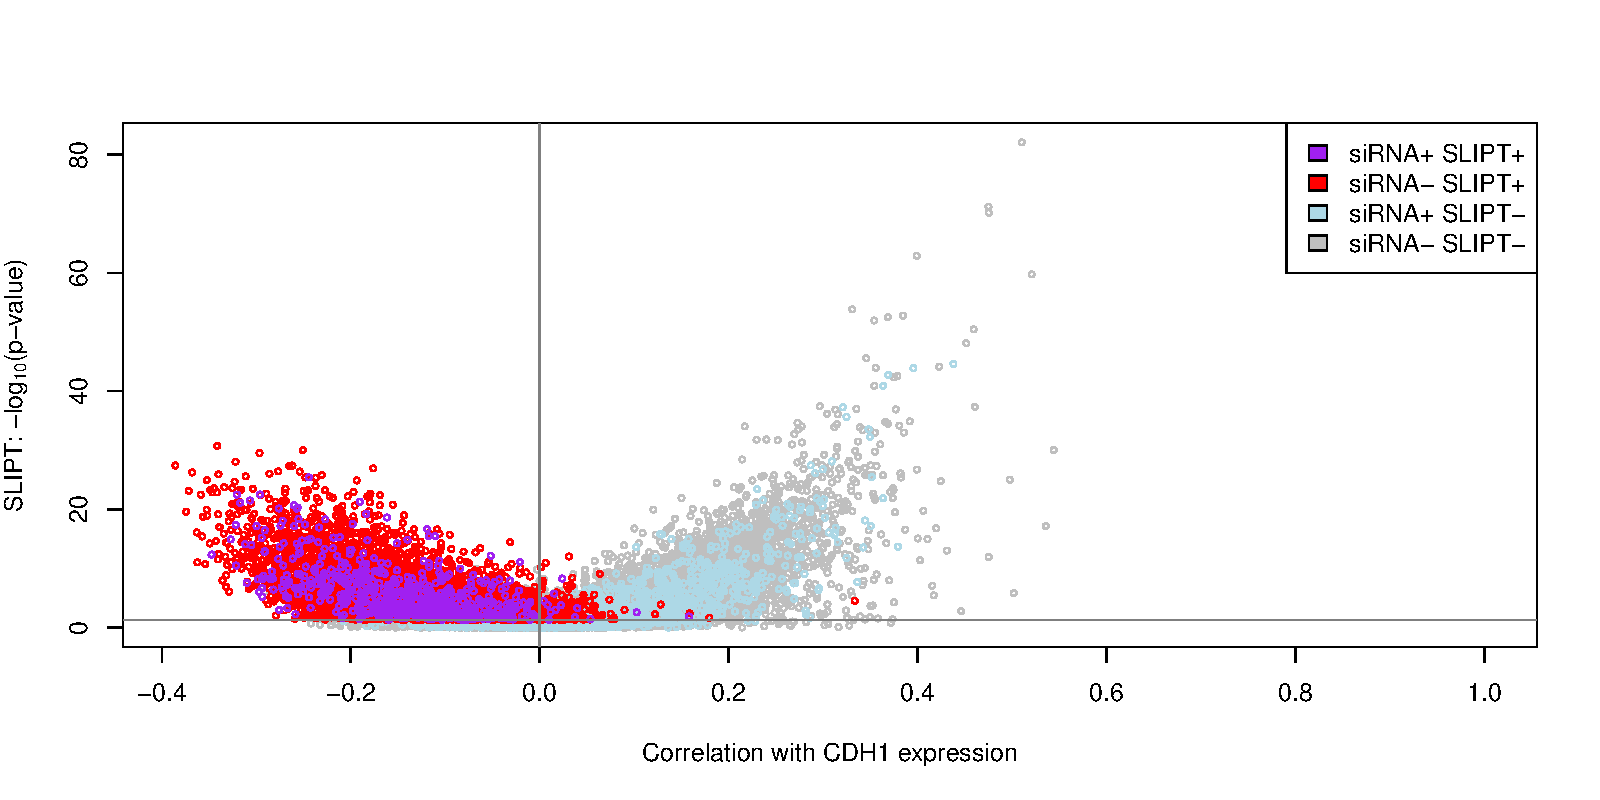
\includegraphics{exprSLIPT_siRNA_vs_Correlation_with_CDH1_nlp.pdf}
   }
   \end{center}
   \caption[Comparison of  SLIPT and siRNA genes with correlation]{\small \textbf{Comparison of  \gls{SLIPT} and \gls{siRNA} genes with correlation.} The $\chi^2$ p-values for genes tested by \gls{SLIPT} (in \gls{TCGA} breast cancer) \glslink{gene expression}{expression} analysis were compared against Pearson correlation of \gls{gene expression} with \textit{CDH1}. Genes detected by \gls{SLIPT} or \gls{siRNA} are coloured according to the legend. 
}
\label{fig:compare_points_correlation_SL}
%\end{mdframed}
\end{figure*}

\subsection{Comparison with Correlation} \label{chapt3:compare_correlation} 

Another potential means to triage drug target candidates is by correlation of \glslink{gene expression}{expression} profiles with \textit{CDH1}. Correlation with \textit{CDH1} was compared to \gls{SLIPT} and \gls{siRNA} results in Figure~\ref{fig:compare_points_correlation_SL}. The genes not detected by \gls{SLIPT} (including \gls{siRNA} candidates) included genes with non-significant \gls{SLIPT} p-values. As expected, these genes were distributed around a correlation of zero. Genes with higher correlation with \textit{CDH1} (either direction) were more significant, although there were exceptions to this trend and larger positive correlations than negative correlations. The majority of \gls{SLIPT} candidates had negative correlations, particularly genes detected by both approaches, although these were typically weak correlations and are unlikely to be sufficient to detect such genes on their own. This is supported by simulation results in Section~\ref{chapt5:compare_methods}.

%\label{fig:compare_points_correlation_SL}


There were not strong positive correlations with \textit{CDH1} among \gls{siRNA} candidates, consistent with previous findings that co-expression was not predictive of \glspl{synthetic lethal} \citep{Jerby2014, Lu2015}. Negative correlation may not be indicative of \glspl{synthetic lethal} either as many \gls{siRNA} candidates also had positive correlations. The \gls{SLIPT} methodology has shown to detect genes with both positive and negative correlations, although it does appear to preferentially detect negatively correlated genes to some extent. These findings were replicated with the \acrshort{mtSLIPT} approach against \textit{CDH1} \gls{mutation} (in Appendix Figure~\ref{fig:compare_points_correlation_mtSL}), although the range of the $\chi^2$ p-values differs due to lower sample size for \gls{mutation} analysis.

\FloatBarrier

The apparent tendency for genes detected by \gls{SLIPT} or \gls{siRNA} to have negative correlations with \textit{CDH1} \glslink{gene expression}{expression} was not due to the smaller number of genes in these groups. The distribution of \textit{CDH1} correlations differed across these gene groups (as shown by Figure~\ref{fig:compare_correlation_SL} and Appendix Figure~\ref{fig:compare_correlation_mtSL}) and tended to be lower in \gls{SLIPT} candidates (as supported by \gls{ANOVA} in Table~\ref{tab:compare_correlation_SL}). However, these are relatively weak correlations and further triage of gene candidates by correlation is not suitable. The genes detected both \gls{SLIPT} and \gls{siRNA} did not differ from \gls{SLIPT} genes and the number of positively correlated \gls{SLIPT} genes was very small.The use of correlation itself is also less effective than \gls{SLIPT} to predict \gls{synthetic lethal} partners in the first place (as shown in Section~\ref{chapt5:compare_correlation}).

\begin{figure*}[!htp]
%\begin{mdframed}
\begin{center}
  \resizebox{0.75 \textwidth}{!}{
    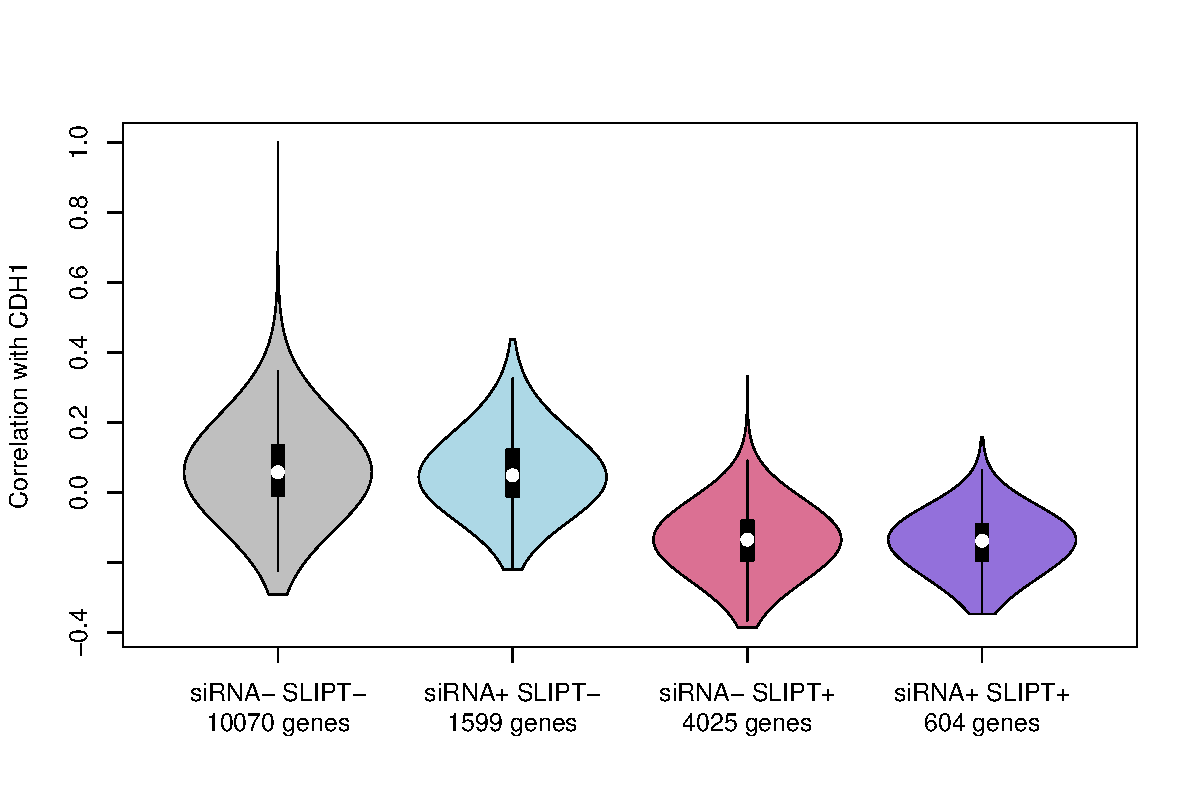
\includegraphics{vioplotx_exprSLIPT_siRNA_vs_CDH1_Correlation_with_CDH1.pdf}
   }
   \end{center}
   \caption[Comparison of SLIPT and siRNA genes with correlation]{\small \textbf{Comparison of  \gls{SLIPT} and \gls{siRNA} genes with correlation.} Genes detected as candidate \gls{synthetic lethal} partners by \gls{SLIPT} (in \gls{TCGA} breast cancer) \glslink{gene expression}{expression} analysis and experimental screening (with \gls{siRNA}) were compared against Pearson correlation of \gls{gene expression} with \textit{CDH1}. There were significant differences in correlation between gene groups (as shown in Table~\ref{tab:compare_correlation_SL}). 
}
\label{fig:compare_correlation_SL}
%\end{mdframed}
\end{figure*}

\begin{table*}[!htb]
\caption{\acrshort{ANOVA} for synthetic lethality and correlation with \textit{CDH1}}
\label{tab:compare_correlation_SL}
\noindent\makebox[\textwidth][c]{%               %centering
\resizebox{0.8 \textwidth}{!}{
\begin{threeparttable}
\begin{tabular}{lccccc}
\hline
                 & DF & Sum Squares & Mean Squares & F-value & p-value \\
\hline
\rowcolor{black!10}
siRNA              &     1    &    0.027     &    0.027     &    2.8209    &    0.09306 \\
\rowcolor{black!5}
SLIPT              &     1    &    134.603    &    134.603    &    14115.9824    &    $<$0.0001 \\
\rowcolor{black!10}
siRNA$\times$SLIPT     &     1    &    0.000      &    0.000      &   0.0073     &    0.93212 \\
\hline
\end{tabular}
\begin{tablenotes}
\raggedright \small
Analysis of variance for correlation with \textit{CDH1} against \gls{synthetic lethal} detection approaches (with an interaction term). Only genes tested by both methods were included in this analysis.
\end{tablenotes}
\end{threeparttable}
}
}
\end{table*} 

\FloatBarrier

\subsection{Comparison with Primary Screen Viability} \label{chapt3:compare_viability}

A similar comparison of \gls{SLIPT} results was made with the viability ratio (\textit{CDH1}$^{-/-}$ \gls{mutant} to \gls{wild-type}) of MCF10A cells in the primary \gls{siRNA} screen performed by \citet{Telford2015}. The significance and viability thresholds used for \gls{SLIPT} and \gls{siRNA} detection of \gls{synthetic lethal} candidate partners of \textit{CDH1} are shown in Figure~\ref{fig:compare_points_viability_SL}. Not all of the genes below the viability  thresholds were necessarily selected to be candidate partners, however, as additional criteria were used in each case: directional criteria as for \gls{SLIPT} (see Section~\ref{methods:SLIPT}) and minimum\gls{wild-type} viability for \gls{siRNA} \citep{Telford2015}.

\begin{figure*}[!htbp]
%\begin{mdframed}
\begin{center}
  \resizebox{0.8 \textwidth}{!}{
    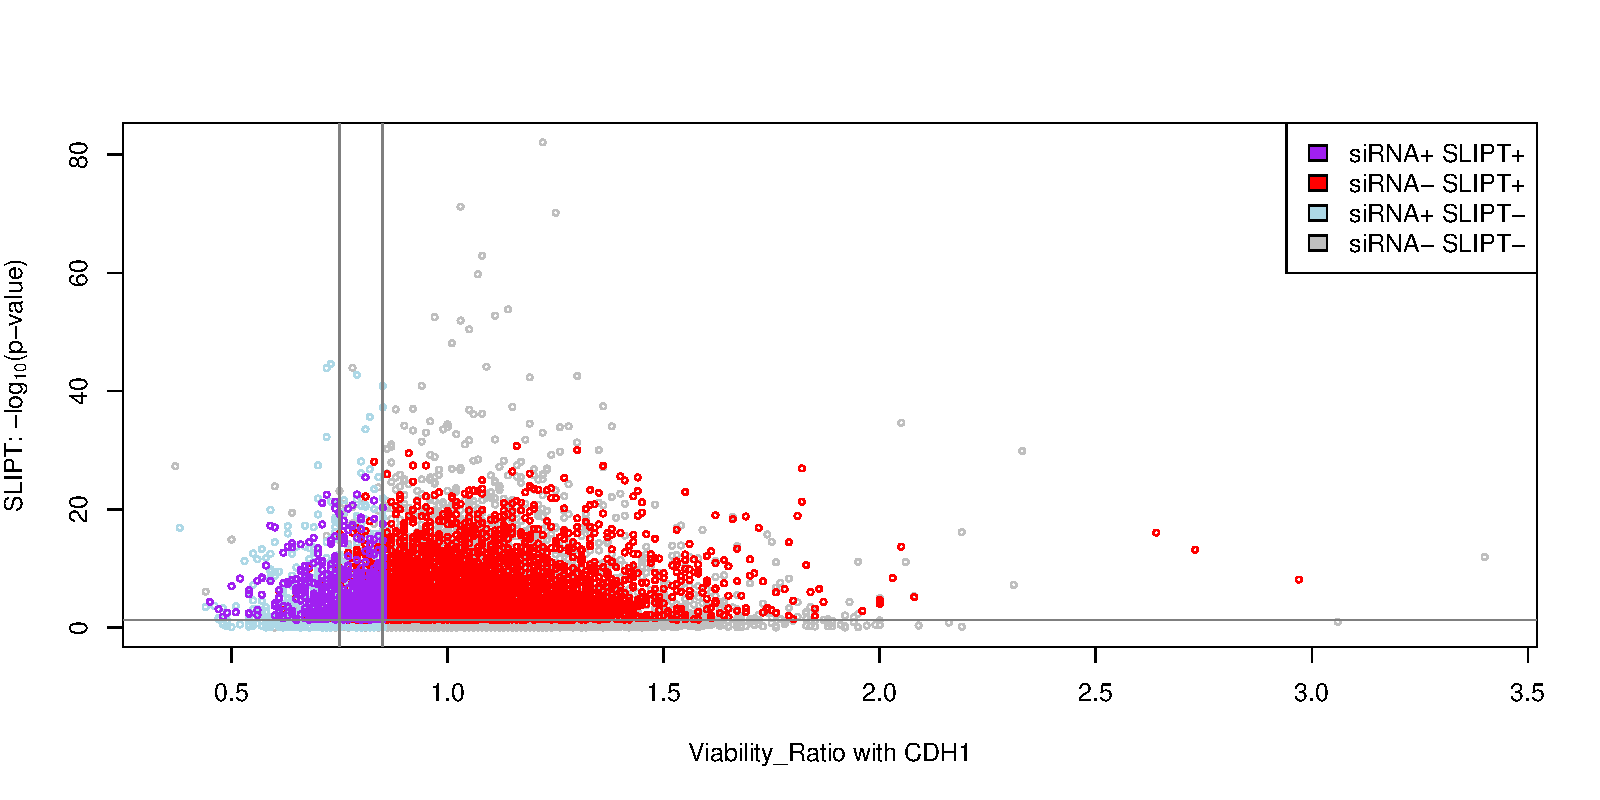
\includegraphics{exprSLIPT_siRNA_vs_Viability_Ratio_with_CDH1_nlp.pdf}
   }
   \end{center}
   \caption[Comparison of SLIPT and siRNA genes with screen viability]{\small \textbf{Comparison of \gls{SLIPT} and \gls{siRNA} genes with screen viability.} The $\chi^2$ p-values (log-scale) for genes tested by \gls{SLIPT} (in \gls{TCGA} breast cancer) were compared against the viability ratio of \textit{CDH1} \gls{mutant} and\gls{wild-type} cells in the primary \gls{siRNA} screen. Genes detected by \gls{SLIPT} or \gls{siRNA} are coloured according to the legend. Lines show the thresholds of significance with \gls{SLIPT} and of viability used by \citet{Telford2015}. % with a grey line for $p=0.05$.
}
\label{fig:compare_points_viability_SL}
%\end{mdframed}
%\end{figure*}

%\begin{figure*}[!htbp]
%\begin{mdframed}
\begin{center}
  \resizebox{0.75 \textwidth}{!}{
    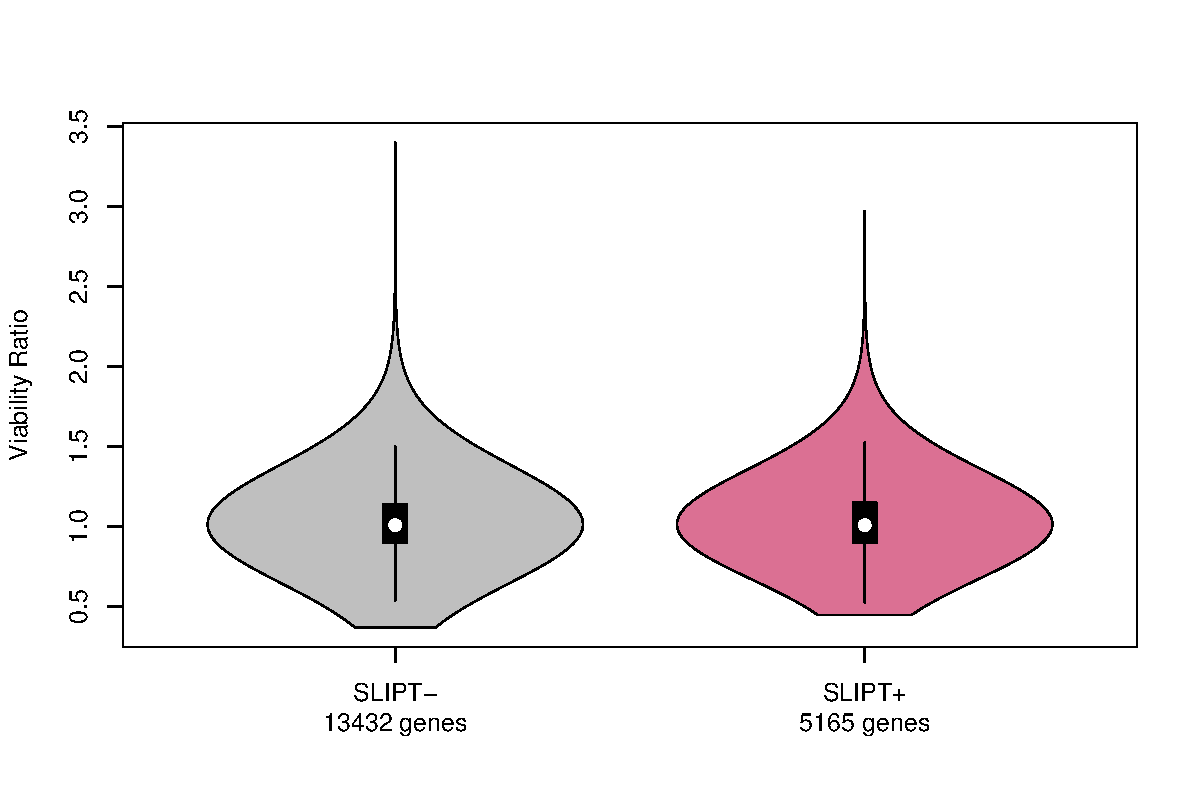
\includegraphics{vioplotx_exprSLIPT_siRNA_vs_Viability_Ratio_with_CDH1.pdf}
   }
   \end{center}
   \caption[Comparison of SLIPT genes with siRNA screen viability]{\small \textbf{Comparison of \gls{SLIPT} genes with \gls{siRNA} screen viability.} Genes detected as candidate \gls{synthetic lethal} partners by \gls{SLIPT} (in \gls{TCGA} breast cancer) \glslink{gene expression}{expression} analysis were compared against the viability ratio of \textit{CDH1} \gls{mutant} and\gls{wild-type} cells in the primary \gls{siRNA} screen. There were clear no differences in viability between genes detected by \gls{SLIPT} and those not detected. The genes identified by \gls{SLIPT} had a higher viability ratio (by t-test: $t=2.1553$, $p=0.03117$), although the effect size was relatively small (mean SLIPT$-$ 1.029, mean SLIPT$+$ 1.037).  % with the differences being primarily due to viability thresholds being used to detect \glspl{synthetic lethal} by \citet{Telford2015}. 
}
\label{fig:compare_viability_SL}
%\end{mdframed}
\end{figure*}

There does not appear to be a clear relationship between \gls{SLIPT} and \gls{siRNA} candidates. The genes detected by one approach but not the other were numerous in Figure~\ref{fig:Venn_allgenes} and Appendix Figure~\ref{fig:Venn_allgenes_mtSL}. These genes detected by one approach are not necessarily near the thresholds for the other. In this respect, the \gls{SLIPT} approach with patient data and the \gls{siRNA} cell line experiments are independent means to identify \gls{synthetic lethal} candidates. While genes detected by both approaches were not necessarily more strongly supported by either, the genes with a viability closer to 1 (no \gls{synthetic lethal} effect) in \gls{siRNA} included those with more significant \gls{SLIPT} p-values, whereas more extreme viability ratios tended to be less significant (as shown by Figure~\ref{fig:compare_points_viability_SL}). However, it should be noted that genes with more moderate viability ratios were more common and \gls{SLIPT} was capable (despite adjusting for multiple testing) of detecting significant genes with extreme viability ratios, particularly those considerably lower than 1. 
%
Lower viability ratios were used by \citet{Telford2015} to detect \gls{synthetic lethal} candidates in the primary screen. However, there was little support for \gls{SLIPT} candidates differing with respect to viability ratio (as shown in Figures~\ref{fig:compare_viability_SL} and~\ref{fig:compare_viability_mtSL}) %However, the genes identified by \gls{SLIPT} had a higher mean viability ratio (by t-test: $t=2.1553$, $p=0.03117$). However, the effect size was small (mean SLIPT$-$ 1.029, mean SLIPT$+$ 1.037)
and the vast majority of \gls{SLIPT} candidate genes did not have different viability in the primary screen to genes not identified by \gls{SLIPT}.


\FloatBarrier

\subsection{Comparison with Secondary siRNA Screen Validation} 
\label{chapt3:secondary_screen}

It should be noted that genes with a lower viability ratio were not necessarily the most strongly supported by experimental screening. The primary screen (with 4 pooled \glspl{siRNA} for each gene) has been used for the majority of comparisons in this thesis because the \glspl{genome}-wide panel of target genes screened enables a large number of genes to be compared with \gls{SLIPT} results from \gls{gene expression} and \glslink{somatic}{somatic} \gls{mutation} analysis. A secondary screen was also performed by \citet{Telford2015} on the isogenic MCF10A breast cell lines to validate the individual (i.e., non-pooled) \glspl{siRNA} separately, with the strongest candidates being those exhibiting \gls{synthetic lethal} viability ratios replicated across independently targeting \glspl{siRNA}. The strongest candidates from the primary screen were subject to a further secondary screen for validation by independent replication with 4 gene knockdowns with different targeting \glspl{siRNA}. This was performed for the top 500 candidates (with the lowest viability ratio) from the primary screen: 482 of these genes were also tested by \gls{SLIPT} in breast cancer.% (and the 486 genes tested by \gls{SLIPT} in stomach cancer).

The secondary screen results show that \gls{SLIPT} candidate genes were more significantly ($p=7.49 \times 10^{-3}$ by Fisher's exact test) more  likely to be validated with detection by more independently targeting \glspl{siRNA} in the secondary screen. Gene detected by \gls{SLIPT} are thus informative of more robust partner genes, in addition to providing support that these interactions are consistent with \glslink{gene expression}{expression} profiles from heterogeneous patient samples across genetic backgrounds. As shown in Table~\ref{tab:secondary_screen}, there is significant %($p=7.49 \times 10^{-3}$ by Fisher's exact test) %$8.67 \times 10^{-3} by \chi^2 (4 df)
association between \gls{SLIPT} candidates and stronger validations of \gls{siRNA} candidates. Since there were more SLIPT$-$ genes among those not validated and more SLIPT$+$ genes among those validated with several \glspl{siRNA}, this supports the use of SLIPT as a \gls{synthetic lethal} discovery procedure which may augment such screening experiments.

\begin{table*}[!ht]
\caption{Comparison of \gls{SLIPT} genes against secondary \gls{siRNA} screen} % in breast cancer}
\label{tab:secondary_screen}
\begin{center}
%\resizebox{\textwidth}{!}{
\begin{threeparttable}
\begin{tabular}{>{\cellcolor{white}}rrcccccl}
                                                                            &                                                                   & \multicolumn{5}{c}{\bfseries Secondary Screen}                                                                                     &                                           \\ \cline{3-7}
\rowcolor{black!10}
                                                                            & \multicolumn{1}{r|}{\cellcolor{white} \textbf{siRNAs}\tnote{*}}   & 0/4                      & 1/4                      & 2/4                     & 3/4                     & \multicolumn{1}{c|}{4/4} & \cellcolor{white} \textbf{Total}          \\ \cline{2-8} 
\rowcolor{black!5}
\multicolumn{1}{r|}{\cellcolor{white}}                                      & \multicolumn{1}{r|}{Observed}                                     & 70                       & 46                       & 31                      & 8                       & \multicolumn{1}{c|}{2}   &  \multicolumn{1}{l|}{}                     \\
\rowcolor{black!10}
\multicolumn{1}{r|}{\cellcolor{white} \multirow{-2}{*}{\bfseries SLIPT$+$}} & \multicolumn{1}{r|}{Expected}                                     & 85                       & 44                       & 10                      & 4                       & \multicolumn{1}{c|}{2}   & \multicolumn{1}{l|}{\multirow{-2}{*}{157}}    \\ \cline{2-8} 
\rowcolor{black!5}
\multicolumn{1}{r|}{\cellcolor{white}}                                      & \multicolumn{1}{r|}{Observed}                                     & 190                      & 90                       & 31                      & 10                      & \multicolumn{1}{c|}{4}   & \multicolumn{1}{l|}{}                     \\
\rowcolor{black!10}
\multicolumn{1}{r|}{\cellcolor{white}\multirow{-2}{*}{\bfseries SLIPT$-$}}  & \multicolumn{1}{r|}{Expected}                                     & 175                      & 91                       & 42                      & 12                      & \multicolumn{1}{c|}{4}   & \multicolumn{1}{l|}{\multirow{-2}{*}{325}} \\ \cline{2-8} 
\rowcolor{black!5}
\cellcolor{white}                                                           & \multicolumn{1}{r|}{\cellcolor{white} \bfseries Total}            & \multicolumn{1}{c}{280} & \multicolumn{1}{c}{136} & \multicolumn{1}{c}{52} & \multicolumn{1}{c}{18} & \multicolumn{1}{c|}{6}   & \multicolumn{1}{l|}{482}                  \\ \cline{3-8} 
\end{tabular} 
\begin{tablenotes}
\raggedright \small
\item[*] Number of \glspl{siRNA} (targeting the same gene) to successfully reproduce \glpls{synthetic lethal} in MCF10A cell lines \citep{Telford2015}

\end{tablenotes}
\end{threeparttable}
%}
\end{center}
\end{table*}

While the individual genes detected by either approach do not necessarily match (and are potentially false-positives), the biological functions important in \textit{CDH1} deficient cancers and potential mechanisms for specific targeting of them can be further supported by pathway analysis of the gene detected by either method. The genes detected by both approaches may therefore be more informative at the pathway level, where it is less likely for a pathway to be consistently detected by chance. As the \gls{SLIPT} candidates differ from the \gls{siRNA} candidates (in addition to those detected by both approaches which were more likely to be validated), they can provide information about additional mechanisms by which \textit{CDH1} deficient cancers proliferate, and vulnerabilities that may be exploited against them by using the \gls{synthetic lethal} pathways.

\FloatBarrier

\subsection{Comparison to Primary Screen at Pathway Level}  \label{chapt3:compare_pathway}

\begin{table*}[!hp]
\caption{Pathways for \textit{CDH1} partners from SLIPT and \gls{siRNA}}
\label{tab:Venn_over-representation}
\centering
\resizebox{0.8 \textwidth}{!}{
\begin{tabular}{sl^c^c^c}
\rowstyle{\bfseries}
  Predicted only by \gls{SLIPT} (4025 genes) & Pathway Size & Genes Identified & p-value (\gls{FDR}) \\ 
  \hline
  \rowcolor{Cluster_Red!20}
  Eukaryotic Translation Elongation &  80 &  75 & $1.5 \times 10^{-182}$ \\
  \rowcolor{Cluster_Red!15} 
  Peptide chain elongation &  77 &  72 & $2.9 \times 10^{-176}$ \\
  \rowcolor{Cluster_Red!20} 
  Viral \acrshort{mRNA} Translation &  75 &  70 & $4.9 \times 10^{-172}$ \\
  \rowcolor{Cluster_Red!15} 
  Eukaryotic Translation Termination &  76 &  70 & $5.9 \times 10^{-170}$ \\
  \rowcolor{Cluster_Red!20} 
  Formation of a pool of free 40S subunits &  87 &  74 & $9.5 \times 10^{-166}$ \\
  \rowcolor{Cluster_Red!15} 
  Nonsense Mediated Decay independent of the Exon Junction Complex &  81 &  70 & $1.2 \times 10^{-160}$ \\
  \rowcolor{Cluster_Red!20} 
  L13a-mediated translational silencing of Ceruloplasmin \glslink{gene expression}{expression} &  97 &  75 & $3.8 \times 10^{-155}$ \\
  \rowcolor{Cluster_Red!15} 
  3' -UTR-mediated translational regulation &  97 &  75 & $3.8 \times 10^{-155}$ \\
  \rowcolor{Cluster_Red!20} 
  GTP hydrolysis and joining of the 60S ribosomal subunit &  98 &  75 & $6.0 \times 10^{-154}$ \\
  \rowcolor{Cluster_Red!15} 
  Nonsense-Mediated Decay &  96 &  73 & $5.2 \times 10^{-150}$ \\
  \rowcolor{Cluster_Red!20} 
  Nonsense Mediated Decay enhanced by the Exon Junction Complex &  96 &  73 & $5.2 \times 10^{-150}$ \\
  \rowcolor{Cluster_Red!15} 
  SRP-dependent cotranslational protein targeting to membrane &  97 &  73 & $7.8 \times 10^{-149}$ \\
  \rowcolor{Cluster_Red!20} 
  Eukaryotic Translation Initiation & 105 &  75 & $4.7 \times 10^{-146}$ \\
  \rowcolor{Cluster_Red!15} 
  Cap-dependent Translation Initiation & 105 &  75 & $4.7 \times 10^{-146}$ \\
  \rowcolor{Cluster_Red!20} 
  Translation & 133 &  83 & $4.0 \times 10^{-142}$ \\
  \rowcolor{Cluster_Red!15} 
  Influenza Viral \acrshort{RNA} Transcription and Replication & 102 &  71 & $2.9 \times 10^{-137}$ \\
  \rowcolor{Cluster_Red!20} 
  Influenza Infection & 111 &  74 & $3.7 \times 10^{-137}$ \\
  \rowcolor{Cluster_Red!15} 
  Influenza Life Cycle & 106 &  71 & $2.3 \times 10^{-133}$ \\
  \rowcolor{Cluster_Red!20} 
  Infectious disease & 326 & 125 & $4.2 \times 10^{-120}$ \\
  \rowcolor{Cluster_Red!15} 
  Extracellular matrix organisation & 189 &  77 & $5.4 \times 10^{-95}$ \\
  \hline
  \\
  \rowstyle{\bfseries}
  Detected only by \gls{siRNA} screen (1599 genes) & Pathway Size & Genes Identified & p-value (\gls{FDR}) \\ 
  \hline
  \rowcolor{Cluster_Blue!20}
  Class A/1 (Rhodopsin-like receptors) & 282 &  44 & $1.3 \times 10^{-27}$ \\
  \rowcolor{Cluster_Blue!15} 
  GPCR ligand binding & 363 &  52 & $5.8 \times 10^{-26}$ \\
  \rowcolor{Cluster_Blue!20} 
  G$_{\alpha q}$ signalling events & 159 &  26 & $6.7 \times 10^{-23}$ \\
  \rowcolor{Cluster_Blue!15} 
  Gastrin-CREB signalling pathway via PKC and MAPK & 180 &  27 & $2.0 \times 10^{-21}$ \\
  \rowcolor{Cluster_Blue!20} 
  G$_{\alpha i}$ signalling events & 184 &  27 & $5.3 \times 10^{-21}$ \\
  \rowcolor{Cluster_Blue!15} 
  Downstream signal transduction & 146 &  23 & $7.6 \times 10^{-21}$ \\
  \rowcolor{Cluster_Blue!20} 
  Signalling by PDGF & 172 &  25 & $4.0 \times 10^{-20}$ \\
  \rowcolor{Cluster_Blue!15} 
  Peptide ligand-binding receptors & 175 &  25 & $8.5 \times 10^{-20}$ \\
  \rowcolor{Cluster_Blue!20} 
  Signalling by ERBB2 & 146 &  22 & $1.3 \times 10^{-19}$ \\
  \rowcolor{Cluster_Blue!15} 
  DAP12 interactions & 159 &  23 & $2.6 \times 10^{-19}$ \\
  \rowcolor{Cluster_Blue!20} 
  DAP12 signalling & 149 &  22 & $2.7 \times 10^{-19}$ \\
  \rowcolor{Cluster_Blue!15} 
  Organelle biogenesis and maintenance & 264 &  33 & $5.5 \times 10^{-19}$ \\
  \rowcolor{Cluster_Blue!20} 
  Signalling by NGF & 266 &  33 & $8.2 \times 10^{-19}$ \\
  \rowcolor{Cluster_Blue!15} 
  Downstream signalling of activated FGFR1 & 134 &  20 & $1.1 \times 10^{-18}$ \\
  \rowcolor{Cluster_Blue!20} 
  Downstream signalling of activated FGFR2 & 134 &  20 & $1.1 \times 10^{-18}$ \\
  \rowcolor{Cluster_Blue!15} 
  Downstream signalling of activated FGFR3 & 134 &  20 & $1.1 \times 10^{-18}$ \\
  \rowcolor{Cluster_Blue!20} 
  Downstream signalling of activated FGFR4 & 134 &  20 & $1.1 \times 10^{-18}$ \\
  \rowcolor{Cluster_Blue!15} 
  Signalling by FGFR & 146 &  21 & $1.3 \times 10^{-18}$ \\
  \rowcolor{Cluster_Blue!20} 
  Signalling by FGFR1 & 146 &  21 & $1.3 \times 10^{-18}$ \\
  \rowcolor{Cluster_Blue!15} 
  Signalling by FGFR2 & 146 &  21 & $1.3 \times 10^{-18}$ \\
  \hline
  \\
  \rowstyle{\bfseries}
  Intersection of \gls{SLIPT} and \gls{siRNA} screen (604 genes) & Pathway Size & Genes Identified & p-value (\gls{FDR}) \\ 
  \hline
  \rowcolor{Cluster_Red!20!Cluster_Blue!20}
  Visual phototransduction &  54 &   9 & $6.9 \times 10^{-10}$ \\
  \rowcolor{Cluster_Red!15!Cluster_Blue!15} 
  G$_{\alpha s}$ signalling events &  48 &   7 & $1.6 \times 10^{-7}$ \\
  \rowcolor{Cluster_Red!20!Cluster_Blue!20} 
  Retinoid metabolism and transport &  24 &   5 & $1.7 \times 10^{-7}$ \\
  \rowcolor{Cluster_Red!15!Cluster_Blue!15} 
  Acyl chain remodelling of PS &  10 &   3 & $6.5 \times 10^{-6}$ \\
  \rowcolor{Cluster_Red!20!Cluster_Blue!20} 
  Transcriptional regulation of white adipocyte differentiation &  51 &   6 & $6.5 \times 10^{-6}$ \\
  \rowcolor{Cluster_Red!15!Cluster_Blue!15} 
  Chemokine receptors bind chemokines &  22 &   4 & $6.5 \times 10^{-6}$ \\
  \rowcolor{Cluster_Red!20!Cluster_Blue!20} 
  Signalling by NOTCH4 &  11 &   3 & $6.9 \times 10^{-6}$ \\
  \rowcolor{Cluster_Red!15!Cluster_Blue!15} 
  Defective EXT2 causes exostoses 2 &  11 &   3 & $6.9 \times 10^{-6}$ \\
  \rowcolor{Cluster_Red!20!Cluster_Blue!20} 
  Defective EXT1 causes exostoses 1, TRPS2 and CHDS &  11 &   3 & $6.9 \times 10^{-6}$ \\
  \rowcolor{Cluster_Red!15!Cluster_Blue!15} 
  Platelet activation, signalling and aggregation & 146 &  12 & $6.9 \times 10^{-6}$ \\
  \rowcolor{Cluster_Red!20!Cluster_Blue!20} 
  Phase 1 - Functionalisation of compounds &  41 &   5 & $1.3 \times 10^{-5}$ \\
  \rowcolor{Cluster_Red!15!Cluster_Blue!15} 
  Amine ligand-binding receptors &  13 &   3 & $1.7 \times 10^{-5}$ \\
  \rowcolor{Cluster_Red!20!Cluster_Blue!20} 
  Acyl chain remodelling of PE &  14 &   3 & $2.4 \times 10^{-5}$ \\
  \rowcolor{Cluster_Red!15!Cluster_Blue!15} 
  Signalling by GPCR & 300 &  23 & $2.4 \times 10^{-5}$ \\
  \rowcolor{Cluster_Red!20!Cluster_Blue!20} 
  Molecules associated with elastic fibres &  29 &   4 & $2.6 \times 10^{-5}$ \\
  \rowcolor{Cluster_Red!15!Cluster_Blue!15} 
  DAP12 interactions & 128 &  10 & $2.6 \times 10^{-5}$ \\
  \rowcolor{Cluster_Red!20!Cluster_Blue!20} 
  Cytochrome P$_{450}$ - arranged by substrate type &  30 &   4 & $3.2 \times 10^{-5}$ \\
  \rowcolor{Cluster_Red!15!Cluster_Blue!15} 
  GPCR ligand binding & 147 &  11 & $3.8 \times 10^{-5}$ \\
  \rowcolor{Cluster_Red!20!Cluster_Blue!20} 
  Acyl chain remodelling of PC &  16 &   3 & $4.0 \times 10^{-5}$ \\
  \rowcolor{Cluster_Red!15!Cluster_Blue!15} 
  Response to elevated platelet cytosolic Ca$^{2+}$ &  66 &   6 & $4.2 \times 10^{-5}$ \\ 
  \hline
\end{tabular}
}
\end{table*}

These pathway over-representation analyses (performed as described in Section~\ref{methods:enrichment}) correspond to genes separated into \gls{SLIPT} or \gls{siRNA} screen candidates unique to either method or detected by both (Table~\ref{tab:Venn_over-representation}). The \gls{SLIPT}-specific gene candidates were involved most strongly with translational and immune regulatory pathways, although extracellular matrix pathways were also supported. These pathways were largely consistent with those identified in Table~\ref{tab:pathway_exprSL} and in the clustering analysis (Table~\ref{tab:pathway_clusters}). The genes detected only by the \gls{siRNA} screen had over-represent\-ation of cell signalling pathways, including many containing genes known to be involved in cancer (e.g., MAPK, PDGF, ERBB2, and FGFR), with the detection of Class A GPCRs supporting the independent analyses by \citet{Telford2015}. The intersection of computational and experimental \gls{synthetic lethal} partners of \textit{CDH1} had stronger evidence for over-represent\-ation of \gls{GPCR} pathways and more specific subclasses, such as visual phototransduction ($p=6.9 \times 10^{-10}$) and G$_{\alpha s}$ signalling events ($p=1.7 \times 10^{-7}$), than other signalling pathways.

The pathway analysis for \acrshort{mtSLIPT} against \textit{CDH1} \glspl{mutation} (in Table~\ref{tab:Venn_over-representation_mtSL}) had concordant results for both \acrshort{mtSLIPT}-specific and \gls{siRNA}-specific pathways. While the specific pathway composition of the intersection of these analyses differed from \gls{SLIPT} against low \textit{CDH1} \glslink{gene expression}{expression}, signalling pathways including \glspl{GPCR}, NOTCH, EERB2, PDGF, and SCF-KIT. These findings indicate the signalling pathways are among the most suitable vulnerability to exploit in targeting \textit{CDH1} deficient tumours as they can be detected in both a patient cohort (with \gls{TCGA} \glslink{gene expression}{expression} data) and tested in a laboratory system. However, it is possible that the isolated experimental system is set up to preferentially detect kinase singalling pathways (which are amenable to pharmacological inhibition and translation to the clinic) and the other pathways identified by \gls{SLIPT} may still be informative of the role of \textit{CDH1} loss of function in cancers or mechanisms by which further gene loss leads to specific inviability.


%%appendix
%\label{tab:Venn_over-representation_mtSL}

\FloatBarrier

\subsubsection{Resampling Genes for Pathway Enrichment} \label{chapt3:compare_pathway_perm}

Comparisons of genes between experimental screen candidates and prediction from \gls{TCGA} \glslink{gene expression}{expression} data were less consistent than comparisons of pathways. However, this is not unexpected, since \gls{synthetic lethal} pathways are more robustly conserved \citep{Dixon2008} and the computational approach using patient samples from complex tumour microenvironment has considerably different strengths to an experimental screen \citep{Telford2015} based on genetically homogenous cell line models in an isolated laboratory environment. For instance, it is unlikely for immune signalling to be detected in an isolated cell culture system.

\begin{figure}[!ht]
%\begin{mdframed}
  \centering
  \resizebox{0.5 \columnwidth}{!}{
    \includegraphics{sample_size_dist_exprSL_1M_Pub.png}
   }
   \caption[Resampled intersection of SLIPT and \gls{siRNA} candidates]{\small \textbf{Resampled intersection of \gls{SLIPT} and \gls{siRNA} candidates.} Resampling analysis of intersect size from genes detected by \gls{SLIPT} and \gls{siRNA} screening approaches over 1 million replicates. The proportion of expected intersection sizes for random samples below or above the observed intersection size respectively, lacking significant over-represent\-ation or depletion of \gls{siRNA} screen candidates within the \gls{SLIPT} predictions for \textit{CDH1}.
   %However, the pathway composition of this intersect may still be informative. %%covered in text
}
\label{fig:perm_sample}
%\end{mdframed}
\end{figure}

The overlap between \gls{synthetic lethal} candidates from \gls{bioinformatics} \gls{SLIPT} predictions and \gls{siRNA} screening has raised other questions, including whether the pathways over-represented would be expected by chance. This of particular concern since the \gls{siRNA} candidate genes themselves are highly over-represented for particular pathways (e.g., \glspl{GPCR}) so selecting any intersect with them could be enriched for these pathways. Another pathway-based approach is to test whether pathways are over-represented in randomly sampled genes, comparing many ``resamplings'' or ``permutations'' of these genes to the enrichment statistics observed for these pathways in the \gls{SLIPT} candidates and their intersection with the \gls{siRNA} hits shows whether we detect these pathways more than we expect by chance (as described in Section~\ref{methods:permutation}). 

Of particular concern are the over-represented pathways in genes detected by both methods. Pathway over-representation alone does not detect whether \gls{SLIPT} predicted genes or \gls{siRNA} candidates are enriched within each other. This resampling analysis therefore detects whether over-represented pathways were detected by \gls{SLIPT} independently of their over-representation among \gls{siRNA} candidates (without assuming an underlying test statistic distribution).

A resampling approach is also applicable to testing whether the number of genes detected by each approach significantly intersected. As shown in Figure~\ref{fig:perm_sample}, resampling did not find evidence of significant depletion or over-represent\-ation for experimental \gls{synthetic lethal} candidate genes in the computationally predicted \gls{synthetic lethal} partners of \textit{CDH1}, and thus the observed overlap may be due to chance. This is consistent with previous findings (see Figure~\ref{fig:Venn_allgenes}) and does not preclude pathway relationships being supported by resampling.

A permutation analysis was performed to resample the genes tested by both approaches to investigate whether the observed pathway over-represent\-ation could have occurred in a randomly selected sample of genes from the experimental candidates, that is, whether the pathway predictions from \gls{SLIPT} could be expected by chance (as described in Sections~\ref{methods:venn_analysis} and~\ref{methods:permutation}).
%The observed 604 genes detected by both approaches (in Figure~\ref{fig:Venn_allgenes}) was not a significantly over-represent\-ation ($p = 0.12982$) or depletion ($p = 0.85841$) of computationally predicted \gls{synthetic lethal} partners of \textit{CDH1} among experimental \gls{synthetic lethal} candidates (in Figure~\ref{fig:perm_sample}). This reinforces the results of the $\chi^2$ analysis,
While the number of \gls{siRNA} candidate genes also detected by \gls{SLIPT} was not statistically significant ($p=0.281$), this may be due to the vastly different limitations of the approaches and the correlation structure of \gls{gene expression} not being independent (as assumed for multiple testing procedures). The  intersection may still be functionally relevant to \textit{CDH1}-deficient cancers, such as the pathway data in Table~\ref{tab:Venn_over-representation}. The resampling analysis for pathways was compared to the pathway over-represent\-ation for \gls{SLIPT} predicted \gls{synthetic lethal} partners in Table~\ref{tab:pathway_perm}. Similarly, the pathway resampling for intersection between \gls{SLIPT} predictions and experimental screen candidates was compared to pathway over-represent\-ation in Table~\ref{tab:pathway_perm_overlap} for intersection with \gls{siRNA} data.

The pathway resampling approach for \gls{SLIPT}-specific gene candidates (Table~\ref{tab:pathway_perm}) replicates the gene set over-represent\-ation analysis for all \gls{SLIPT} genes, detecting evidence of \gls{synthetic lethal} pathways for \textit{CDH1} in translational, immune, and cell signalling pathways including  G$_{\alpha i}$ signalling, \gls{GPCR} downstream signalling, and chemokine receptor binding. While the immune and signal transduction pathways were not significantly over-represented in the resampling analysis, the results for the two approaches were largely consistent for translation and post-transcriptional gene regulation, supporting gene set over-represent\-ation of the \gls{SLIPT}-specific pathways in Table~\ref{tab:pathway_perm}. In particular, some of the most significantly over-represented pathways had higher observed $\chi^2$ values than any of the 1 million random permutations. Similar pathways were also replicated by permutation analysis for mt\gls{SLIPT} candidate partners against \textit{CDH1} \gls{mutation} (shown in Table~\ref{tab:pathway_perm_mtSL}). This shows that many of the pathways detected specifically by \gls{SLIPT} are replicated by permutation procedures and that the permutation approach is capable of detecting many of the most strongly over-represented pathways. 


\begin{table*}[!ht]
\caption{Pathways for \textit{CDH1} partners from SLIPT}
\label{tab:pathway_perm}
\centering
\resizebox{0.8 \textwidth}{!}{
\begin{threeparttable}
\begin{tabular}{sl^c^c}
\rowstyle{\bfseries}
 Reactome Pathway & Over-representation & Permutation \\ 
  \hline
  \rowcolor{Cluster_Red!20} 
  \textbf{Eukaryotic Translation Elongation} & $1.3 \times 10^{-207}$ & $< 1.241 \times 10^{-5}$  \\
  \rowcolor{Cluster_Red!15}  
   \textbf{Peptide chain elongation} & $5.6 \times 10^{-201}$ & $< 1.241 \times 10^{-5}$  \\
  \rowcolor{Cluster_Red!20}  
   \textbf{Viral \acrshort{mRNA} Translation} & $1.2 \times 10^{-196}$ & $< 1.241 \times 10^{-5}$  \\
  \rowcolor{Cluster_Red!15}  
   \textbf{Eukaryotic Translation Termination} & $1.2 \times 10^{-196}$ & $< 1.241 \times 10^{-5}$  \\
  \rowcolor{Cluster_Red!20}  
   \textbf{Formation of a pool of free 40S subunits} & $3.7 \times 10^{-194}$ & $< 1.241 \times 10^{-5}$  \\
  \rowcolor{Cluster_Red!15}  
   \textbf{Nonsense Mediated Decay independent of the Exon Junction Complex} & $5.3 \times 10^{-187}$ & $< 1.241 \times 10^{-5}$  \\
  \rowcolor{Cluster_Red!20}  
   \textbf{L13a-mediated translational silencing of Ceruloplasmin \glslink{gene expression}{expression}} & $9.6 \times 10^{-183}$ & $< 1.241 \times 10^{-5}$  \\
  \rowcolor{Cluster_Red!15}  
   \textbf{3' -UTR-mediated translational regulation} & $9.6 \times 10^{-183}$ & $< 1.241 \times 10^{-5}$  \\
  \rowcolor{Cluster_Red!20}  
   \textbf{GTP hydrolysis and joining of the 60S ribosomal subunit} & $1.9 \times 10^{-181}$ & $< 1.241 \times 10^{-5}$  \\
  \rowcolor{Cluster_Red!15}  
   \textbf{Nonsense-Mediated Decay} & $6.2 \times 10^{-176}$ & $< 1.241 \times 10^{-5}$  \\
  \rowcolor{Cluster_Red!20}  
   \textbf{Nonsense Mediated Decay enhanced by the Exon Junction Complex} & $6.2 \times 10^{-176}$ & $< 1.241 \times 10^{-5}$  \\
  \rowcolor{Cluster_Red!15}  
  Adaptive Immune System & $6.5 \times 10^{-174}$ & $0.15753$ \\
  \rowcolor{Cluster_Red!20}  
  \textbf{Eukaryotic Translation Initiation} & $5.7 \times 10^{-173}$ & $< 1.241 \times 10^{-5}$  \\
  \rowcolor{Cluster_Red!15}  
  \textbf{Cap-dependent Translation Initiation} & $5.7 \times 10^{-173}$ & $< 1.241 \times 10^{-5}$  \\
  \rowcolor{Cluster_Red!20}  
  \textbf{SRP-dependent cotranslational protein targeting to membrane} & $2.0 \times 10^{-171}$ & $< 1.241 \times 10^{-5}$  \\
  \rowcolor{Cluster_Red!15}  
  \textbf{Translation} & $6.1 \times 10^{-170}$ & $< 1.241 \times 10^{-5}$  \\
  \rowcolor{Cluster_Red!20}  
  Infectious disease & $1.6 \times 10^{-166}$ & $0.23231$ \\
  \rowcolor{Cluster_Red!15}  
  \textbf{Influenza Infection} & $1.9 \times 10^{-163}$ & $< 1.241 \times 10^{-5}$  \\
  \rowcolor{Cluster_Red!20}  
  \textbf{Influenza Viral \acrshort{RNA} Transcription and Replication} & $1.9 \times 10^{-160}$ & $< 1.241 \times 10^{-5}$  \\
  \rowcolor{Cluster_Red!15}  
  \textbf{Influenza Life Cycle} & $2.5 \times 10^{-156}$ & $< 1.241 \times 10^{-5}$  \\
  \rowcolor{Cluster_Red!20}  
  \textit{Extracellular matrix organisation} & $1.1 \times 10^{-152}$ & $0.071761$ \\
  \rowcolor{Cluster_Red!15}  
  GPCR ligand binding & $1.1 \times 10^{-143}$ & $0.55801$ \\
  \rowcolor{Cluster_Red!20}  
  Class A/1 (Rhodopsin-like receptors) & $1.5 \times 10^{-142}$ & $0.58901$ \\
  \rowcolor{Cluster_Red!15}  
  \textit{GPCR downstream signalling} & $7.6 \times 10^{-140}$ & $0.098357$ \\
  \rowcolor{Cluster_Red!20}  
  Haemostasis & $1.9 \times 10^{-134}$ & $0.27059$ \\
  \rowcolor{Cluster_Red!15}  
  Developmental Biology & $2.0 \times 10^{-123}$ & $0.52737$ \\
  \rowcolor{Cluster_Red!20}  
  Metabolism of lipids and lipoproteins & $3.3 \times 10^{-120}$ & $0.724$ \\
  \rowcolor{Cluster_Red!15}  
  Cytokine Signalling in Immune system & $2.6 \times 10^{-119}$ & $0.39661$ \\
  \rowcolor{Cluster_Red!20}  
  Peptide ligand-binding receptors & $3.7 \times 10^{-109}$ & $0.61102$ \\
  \rowcolor{Cluster_Red!15}  
  \textbf{G$_{\alpha i}$ signalling events} & $8.9 \times 10^{-100}$ & $< 1.241 \times 10^{-5}$  \\
  \iffalse
  \rowcolor{Cluster_Red!20}  
  Axon guidance & $1.4 \times 10^{-96}$ & $0.66232$ \\
  \rowcolor{Cluster_Red!15}  
  Platelet activation, signalling and aggregation & $3.7 \times 10^{-94}$ & $0.29662$ \\
  \rowcolor{Cluster_Red!20}  
  Immunoregulatory interactions between a Lymphoid and a non-Lymphoid cell & $1.4 \times 10^{-93}$ & $< 1.241 \times 10^{-5}$  \\
  \rowcolor{Cluster_Red!15}  
  Formation of the ternary complex, and subsequently, the 43S complex & $7.0 \times 10^{-91}$ & $< 1.241 \times 10^{-5}$  \\
  \rowcolor{Cluster_Red!20}  
  Translation initiation complex formation & $9.6 \times 10^{-87}$ & $6.8667 \times 10^{-5}$  \\
  \rowcolor{Cluster_Red!15}  
  Ribosomal scanning and start codon recognition & $9.6 \times 10^{-87}$ & $6.8667 \times 10^{-5}$  \\
  \rowcolor{Cluster_Red!20}  
  \begin{tabular}[c]{@{}l@{}}Activation of the \acrshort{mRNA} upon binding of the cap-binding complex and eIFs,\\and subsequent binding to 43S \end{tabular} & $8.7 \times 10^{-86}$ & $6.8667 \times 10^{-5}$  \\
  \rowcolor{Cluster_Red!15}  
  Chemokine receptors bind chemokines & $5.1 \times 10^{-82}$ & $< 1.241 \times 10^{-5}$  \\
  \rowcolor{Cluster_Red!20}  
  Signalling by NGF & $1.2 \times 10^{-81}$ & $0.37142$ \\
  \rowcolor{Cluster_Red!15}  
  Toll-Like Receptors Cascades & $5.3 \times 10^{-80}$ & $0.63013$ \\
  \rowcolor{Cluster_Red!20}  
  Interferon gamma signalling & $6.3 \times 10^{-80}$ & $0.61493$ \\
  \rowcolor{Cluster_Red!15}  
  Transmembrane transport of small molecules & $5.3 \times 10^{-78}$ & $0.21216$ \\
  \rowcolor{Cluster_Red!20}  
  Signalling by Rho GTPases & $1.1 \times 10^{-77}$ & $0.078314$ \\
  \rowcolor{Cluster_Red!15}  
  Degradation of the extracellular matrix & $7.3 \times 10^{-77}$ & $0.769$ \\
  \rowcolor{Cluster_Red!20}  
  Interferon Signalling & $1.1 \times 10^{-76}$ & $0.18211$ \\
  \rowcolor{Cluster_Red!15}  
  NGF signalling via TRKA from the plasma membrane & $1.4 \times 10^{-74}$ & $0.60076$ \\
  \rowcolor{Cluster_Red!20}  
  Gastrin-CREB signalling pathway via PKC and MAPK & $3.1 \times 10^{-74}$ & $0.93109$ \\
  \rowcolor{Cluster_Red!15}  
  Rho GTPase cycle & $3.2 \times 10^{-73}$ & $0.11446$ \\
  \rowcolor{Cluster_Red!20}  
  DAP12 interactions & $2.0 \times 10^{-71}$ & $0.57671$ \\
  \rowcolor{Cluster_Red!15}  
  Cell surface interactions at the vascular wall & $3.3 \times 10^{-71}$ & $0.66232$ \\ 
  \fi
  \hline
\end{tabular}
\begin{tablenotes}
\raggedright \small
Over-representation (hypergeometric test) and Permutation p-values adjusted for multiple tests across pathways (\gls{FDR}). Significant pathways are marked in bold (\gls{FDR} $ < 0.05$) and italics (\gls{FDR} $ < 0.1$).
\end{tablenotes}
\end{threeparttable}
}
\end{table*}

The permutation approach was then also applied to the intersection between computational and experimental candidates. The permutation analysis is testing for consistent detection of pathways was independent of their pre-existing status as experimental candidates. The pathway results for these candidate partners (in Table~\ref{tab:pathway_perm_overlap}) differed between over-represent\-ation and resampling analyses.

Namely, many of the over-represented pathways were not significant in the resampling analysis, including visual phototransduction and retinoic acid signalling, and were likely over-represented in the intersection due to over-represent\-ation in the \gls{siRNA} candidates rather than additional support from \gls{SLIPT}. In contrast, pathways involving defective \textit{EXT1} or \textit{EXT2} genes approach significance after \gls{FDR} adjustment for multiple tests in resampling. Of the highest over-represented pathways in the intersection, only G$_{\alpha s}$ signalling events were supported by both over-represent\-ation and resampling analyses. Other pathways supported by both analyses were cytoplasmic elastic fibre formation, associated HS-GAG protein modification pathways, energy metabolism, and the fibrin clotting cascade.  

\begin{table*}[!htp]
\caption{Pathways for \textit{CDH1} partners from SLIPT and \gls{siRNA} primary screen}
\label{tab:pathway_perm_overlap}
\centering
\resizebox{0.8 \textwidth}{!}{
\begin{threeparttable}
\begin{tabular}{sl^c^c}
\rowstyle{\bfseries}
 Reactome Pathway & Over-representation & Permutation \\ 
  \hline
  \rowcolor{Cluster_Red!20!Cluster_Blue!20} 
  Visual phototransduction & $6.9 \times 10^{-10}$ & $0.91116$  \\
  \rowcolor{Cluster_Red!15!Cluster_Blue!15}  
  \textbf{G$_{\alpha s}$ signalling events} & $1.6 \times 10^{-7}$ & $0.012988$  \\
  \rowcolor{Cluster_Red!20!Cluster_Blue!20}  
  Retinoid metabolism and transport & $1.7 \times 10^{-7}$ & $0.20487$  \\
  \rowcolor{Cluster_Red!15!Cluster_Blue!15}  
  Transcriptional regulation of white adipocyte differentiation & $6.5 \times 10^{-6}$ & $0.38197$  \\
  \rowcolor{Cluster_Red!20!Cluster_Blue!20}  
  Acyl chain remodelling of PS & $6.5 \times 10^{-6}$ & $0.58485$  \\
  \rowcolor{Cluster_Red!15!Cluster_Blue!15}  
  Chemokine receptors bind chemokines & $6.5 \times 10^{-6}$ & $0.97255$  \\
  \rowcolor{Cluster_Red!20!Cluster_Blue!20}  
  \textit{Defective EXT2 causes exostoses 2} & $6.9 \times 10^{-6}$ & $0.056437$  \\
  \rowcolor{Cluster_Red!15!Cluster_Blue!15}  
  \textit{Defective EXT1 causes exostoses 1, TRPS2 and CHDS} & $6.9 \times 10^{-6}$ & $0.056437$  \\
  \rowcolor{Cluster_Red!20!Cluster_Blue!20}  
  Signalling by NOTCH4 & $6.9 \times 10^{-6}$ & $0.15497$  \\
  \rowcolor{Cluster_Red!15!Cluster_Blue!15}  
  Platelet activation, signalling and aggregation & $6.9 \times 10^{-6}$ & $0.53358$  \\
  \rowcolor{Cluster_Red!20!Cluster_Blue!20}  
  Phase 1 - Functionalisation of compounds & $1.3 \times 10^{-5}$ & $0.24836$  \\
  \rowcolor{Cluster_Red!15!Cluster_Blue!15}  
  Amine ligand-binding receptors & $1.7 \times 10^{-5}$ & $0.3195$  \\
  \rowcolor{Cluster_Red!20!Cluster_Blue!20}  
  Acyl chain remodelling of PE & $2.4 \times 10^{-5}$ & $0.7307$  \\
  \rowcolor{Cluster_Red!15!Cluster_Blue!15}  
  Signalling by GPCR & $2.4 \times 10^{-5}$ & $0.9939$  \\
  \rowcolor{Cluster_Red!20!Cluster_Blue!20}  
  \textbf{Molecules associated with elastic fibres} & $2.6 \times 10^{-5}$ & $0.0072929$  \\
  \rowcolor{Cluster_Red!15!Cluster_Blue!15}  
  DAP12 interactions & $2.6 \times 10^{-5}$ & $0.78273$  \\
  \rowcolor{Cluster_Red!20!Cluster_Blue!20}  
  Cytochrome P$_{450}$ - arranged by substrate type & $3.2 \times 10^{-5}$ & $0.87019$  \\
  \rowcolor{Cluster_Red!15!Cluster_Blue!15}  
  GPCR ligand binding & $3.8 \times 10^{-5}$ & $0.99417$  \\
  \rowcolor{Cluster_Red!20!Cluster_Blue!20}  
  Acyl chain remodelling of PC & $4.0 \times 10^{-5}$ & $0.65415$  \\
  \rowcolor{Cluster_Red!15!Cluster_Blue!15}  
  Response to elevated platelet cytosolic Ca$^{2+}$ & $4.2 \times 10^{-5}$ & $0.55461$  \\
  \rowcolor{Cluster_Red!20!Cluster_Blue!20}  
  \textit{Arachidonic acid metabolism} & $4.4 \times 10^{-5}$ & $0.060298$  \\
  \rowcolor{Cluster_Red!15!Cluster_Blue!15}  
  Defective B4GALT7 causes EDS, progeroid type & $4.9 \times 10^{-5}$ & $0.15497$  \\
  \rowcolor{Cluster_Red!20!Cluster_Blue!20}  
  Defective B3GAT3 causes JDSSDHD & $4.9 \times 10^{-5}$ & $0.15497$  \\
  \rowcolor{Cluster_Red!15!Cluster_Blue!15}  
  \textbf{Elastic fibre formation} & $4.9 \times 10^{-5}$ & $0.0019227$  \\
  \rowcolor{Cluster_Red!20!Cluster_Blue!20}  
  \textbf{HS-GAG degradation} & $6.2 \times 10^{-5}$ & $0.017747$  \\
  \rowcolor{Cluster_Red!15!Cluster_Blue!15}  
  Bile acid and bile salt metabolism & $6.2 \times 10^{-5}$ & $0.15497$  \\
  \rowcolor{Cluster_Red!20!Cluster_Blue!20}  
  Netrin-1 signalling & $7.1 \times 10^{-5}$ & $0.95056$  \\
  \rowcolor{Cluster_Red!15!Cluster_Blue!15}  
  \textbf{Integration of energy metabolism} & $7.1 \times 10^{-5}$ & $0.0019287$  \\
  \rowcolor{Cluster_Red!20!Cluster_Blue!20}  
  DAP12 signalling & $7.9 \times 10^{-5}$ & $0.67835$  \\
  \rowcolor{Cluster_Red!15!Cluster_Blue!15}  
  GPCR downstream signalling & $8.1 \times 10^{-5}$ & $0.88678$  \\
  \rowcolor{Cluster_Red!20!Cluster_Blue!20}  
  \textbf{Diseases associated with glycosaminoglycan metabolism} & $8.7 \times 10^{-5}$ & $0.017747$  \\
  \rowcolor{Cluster_Red!15!Cluster_Blue!15}  
  \textbf{Diseases of glycosylation} & $8.7 \times 10^{-5}$ & $0.017747$  \\
  \rowcolor{Cluster_Red!20!Cluster_Blue!20}  
  Signalling by Retinoic Acid & $8.7 \times 10^{-5}$ & $0.13592$  \\
  \rowcolor{Cluster_Red!15!Cluster_Blue!15}  
  Signalling by Leptin & $8.7 \times 10^{-5}$ & $0.15497$  \\
  \rowcolor{Cluster_Red!20!Cluster_Blue!20}  
  Signalling by SCF-KIT & $8.7 \times 10^{-5}$ & $0.73399$  \\
  \rowcolor{Cluster_Red!15!Cluster_Blue!15}  
  Opioid Signalling & $8.7 \times 10^{-5}$ & $0.99417$  \\
  \rowcolor{Cluster_Red!20!Cluster_Blue!20}  
  Signalling by NOTCH & $0.0001$ & $0.26453$  \\
  \rowcolor{Cluster_Red!15!Cluster_Blue!15}  
  Platelet homeostasis & $0.0001$ & $0.55912$  \\
  \rowcolor{Cluster_Red!20!Cluster_Blue!20}  
  Signalling by NOTCH1 & $0.00011$ & $0.13797$  \\
  \rowcolor{Cluster_Red!15!Cluster_Blue!15}  
  Class B/2 (Secretin family receptors) & $0.00011$ & $0.4659$  \\
  \rowcolor{Cluster_Red!20!Cluster_Blue!20}  
  Diseases of Immune System & $0.00013$ & $0.15497$  \\
  \rowcolor{Cluster_Red!15!Cluster_Blue!15}  
  Diseases associated with the TLR signalling cascade & $0.00013$ & $0.15497$  \\
  \rowcolor{Cluster_Red!20!Cluster_Blue!20}  
  A tetrasaccharide linker sequence is required for GAG synthesis & $0.00013$ & $0.33566$  \\
  \rowcolor{Cluster_Red!15!Cluster_Blue!15}  
  Nuclear Receptor transcription pathway & $0.00016$ & $0.22735$  \\
  \rowcolor{Cluster_Red!20!Cluster_Blue!20}  
  \textbf{Formation of Fibrin Clot (Clotting Cascade)} & $0.00016$ & $0.0054639$  \\
  \rowcolor{Cluster_Red!15!Cluster_Blue!15}  
  Syndecan interactions & $0.00016$ & $0.3974$  \\
  \rowcolor{Cluster_Red!20!Cluster_Blue!20}  
  Class A/1 (Rhodopsin-like receptors) & $0.00016$ & $0.99454$  \\
  \rowcolor{Cluster_Red!15!Cluster_Blue!15}  
  HS-GAG biosynthesis & $0.0002$ & $0.37199$  \\
  \rowcolor{Cluster_Red!20!Cluster_Blue!20}  
  Platelet degranulation  & $0.0002$ & $0.39003$  \\
  \rowcolor{Cluster_Red!15!Cluster_Blue!15}  
  EPH-ephrin mediated repulsion of cells & $0.00021$ & $0.6193$  \\ 
  \hline
\end{tabular}
\begin{tablenotes}
\raggedright \small
Over-representation (hypergeometric test) and Permutation p-values adjusted for multiple tests across pathways (\gls{FDR}). Significant pathways are marked in bold (\gls{FDR} $ < 0.05$) and italics (\gls{FDR} $ < 0.1$).
\end{tablenotes}
\end{threeparttable}
}
\end{table*}

Many of the pathways supported in the intersection by permutation analysis were also replicated in the \acrshort{mtSLIPT} analysis of partners tested with \textit{CDH1} \gls{mutation} (in Table~\ref{tab:pathway_perm_overlap_mtSL}), including G$_{\alpha s}$, elastic fibres, HS-GAG, and energy metabolism. While there were differences between the pathways identified by over-representation analysis, those replicated by permutation were highly concordant, supportig the combined use of these pathway approaches to identify \gls{synthetic lethal} gene functions and targets. 

While this indicates that G$_{\alpha s}$ and \gls{GPCR} class A/1 signalling events were significantly detected by both approaches, \gls{GPCR} signalling pathways overall were not. It is likely that \glspl{GPCR} were primarily over-represented in the intersection with the experimental candidates due to strong over-represent\-ation of these pathways in experimental candidates, rather than detection by \gls{SLIPT}, which may be driven by these more specific constituent pathways. 

%% remove paragraph?
However, several pathways, including some immune functions and neurotransmitters, were supported by the resampling analysis (in Tables~\ref{tab:pathway_perm_overlap} and~\ref{tab:pathway_perm_overlap_mtSL}) when the initial pathway over-represent\-ation test was not significant. These functions appear to have been detected by both approaches  more than expected by chance but must be interpreted with caution since they were still not common enough to be detected in pathway over-represent\-ation analysis.

\subsection{Integrating Synthetic Lethal Pathways and Screens}

Based on these results, it appears that computational and experimental approaches to \gls{synthetic lethal} screening for \textit{CDH1} lead to a broader functional characterisation, and many candidate partners, when combined, despite different strengths and limitations. Compared to candidate gene approaches, experimental \glspl{genome}-wide screens are an appealing unbiased strategy for identifying \gls{synthetic lethal} interactions. Since these screens are costly, laborious, and specific to genetic background, computational analysis can augment candidate triage to either reduce the initial panel of screened genes or prioritise validation.

\gls{GPCR} pathways were detected among both computational and experimental \gls{synthetic lethal} candidates, with more support in the experimental screen (Table~\ref{tab:pathway_perm_overlap}). The homogeneous cell line model may be more likely to detect particular pathways. For instance, \gls{SLIPT} identified immune pathways, not expected to be detected in isolated cell culture. \gls{GPCR} signalling was supported in experimental models \cite{Telford2015} with some of these pathways replicated in varied genetic backgrounds of patient samples. These pathways require further investigation such as identification of more specific pathways, higher order interactions, and modes of resistance.

The pathway composition across computational and experimental \gls{synthetic lethal} candidates was informative with over-represent\-ation (Table~\ref{tab:Venn_over-representation}) and supported by resampling analysis (Table~\ref{tab:pathway_perm_overlap}), despite a modest intersection of genes between them (Figure~\ref{fig:Venn_allgenes}).
Either approach may be significant for a pathway in this intersection without being supported by the other: resampling analysis may support pathways that were not over-represent\-ed due to small effect sizes, thus both tests are required for a candidate pathway.
The pathways detected by both over-represent\-ation and resampling are the strongest candidates for further investigation, such as G$_{\alpha s}$ signalling, a strong candidate in prior analyses with a role in the regulation of translation in cancer \cite{Gao2015}, another function supported by \gls{SLIPT} analysis.
%The \gls{bioinformatics} analysis demonstrated here could be integrated into future screening for \glspl{synthetic lethal} in cancer.  

The predicted \gls{synthetic lethal} partners occurred across functionally distinct pathways, including characterised functions of \textit{CDH1}. This diversity is consistent with the wide ranging role of \textit{CDH1} in cell-cell adhesion, cell signalling, and the cytoskeletal structure of epithelial tissues. Pathway structure may be relevant to identifying potential drug targets from \gls{gene expression} signatures, indicating downstream effector genes and mechanisms leading to cell inviability. These distinct \gls{synthetic lethal} gene clusters and pathways may further lead to the elucidation of drug resistance mechanisms.

%%appendix
%\label{tab:pathway_perm_mtSL}
%\label{tab:pathway_perm_overlap_mtSL}

\FloatBarrier

%\subsubsection{Comparison of Candidate SL Pathways}
%committee
%Thus we have identified candidate \gls{synthetic lethal} pathways by gene set over-representation, \gls{metagene} \glspl{synthetic lethal}, and resampled empirical pathway over-representation. The challenge currently under consideration is whether these methods can be compared and which may lead to biologically meaningful or clinically relevant \gls{synthetic lethal} candidate pathways.
%\FloatBarrier

\iffalse

\section{Mutation, Copy Number, and Methylation}

Due to promising \gls{synthetic lethal} data on \gls{mutation} and \acrshort{DNA} copy number analyses \citep{Jerby2014, Lu2015}, these were also investigated to compare genes for \glspl{synthetic lethal} in an analogous manner to \glslink{gene expression}{expression} analyses in the \gls{TCGA} data. Due to the low \glslink{somatic}{somatic} \gls{mutation} rate (and lack of available) \gls{germline} \glspl{mutation} for many genes, it was not possible to detect many double \glspl{mutation} with significantly under-representation in cancers. There were also concerns about using rare \glspl{mutation} with unknown significance or excluding functional \glspl{mutation} by only using those in the exons.
It was possible to compare deletion and duplication of \acrshort{DNA} copy number in a manner analogous to \glslink{gene expression}{expression} quantiles. However, these overlapped poorly with candidate interacting partners from \glslink{gene expression}{expression} analyses and concerns were raised that they may not be relevant to \textit{CDH1} which is typically inactivated in tumours by loss of function \glspl{mutation} or \acrshort{DNA} methylation (PJ Guilford, personal communication).   

DNA methylation data was also prepared for \gls{synthetic lethal} analysis but was discontinued due to computational challenges, expected similarity to \glslink{gene expression}{expression} results, difficulty defining loss of function methylation at a gene level across \gls{CpG} sites, and the concerns raised in the next section. 

\subsection{Synthetic lethality by \acrshort{DNA} copy number}


\fi


\section{Metagene Analysis}  \label{chapt3:metagene_results}
%[include?]

The gene signatures \citep{Gatza2011, Gatza2014} were used to demonstrate to utility of the \gls{metagene} approach for use on a wider range of pathways as was performed with the Reactome \citep{Reactome} pathways as an alternative approach to identification of \gls{synthetic lethal} pathways. \Glspl{metagene} serve as a summary of activity for each pathway. The direction of \glspl{metagene} (derived by the singular value matrix decomposition) is generally arbitrary but care has been taken to ensure that these occur in a direction which reflect overall activation of the pathway (as described in Section~\ref{methods:metagene}). \Glspl{metagene} were derived for well characterised gene signatures in breast cancer \citep{Gatza2011, Gatza2014} to verify that that these pathway signatures are consistent with expected molecular properties of each molecular subtype \citep{Perou2000, Parker2009}. This was performed by examining the pathway \glslink{gene expression}{expression} of these breast cancer gene signatures in \gls{TCGA} \glslink{gene expression}{expression} data. These \glspl{metagene} were also compared to \glslink{somatic}{somatic} \gls{mutation} to evaluate \gls{mutation} as a measure of gene activity in comparison to gene and protein \glslink{gene expression}{expression}.

The gene signatures \citep{Gatza2011, Gatza2014} were used to demonstrate to utility of the \gls{metagene} approach for use on a wider range of pathways. Having established that \glspl{metagene} generated with this procedure reflect gene activity, the \gls{metagene} procedure (in Section~\ref{methods:metagene}) was then applied to the Reactome pathways \citep{Reactome}. These Reactome \glspl{metagene} were used for \gls{synthetic lethal} analysis of pathways with \gls{SLIPT}, directly using pathway activity for identifying \gls{synthetic lethal} pathways with \textit{CDH1}.

\subsection{Pathway Expression} \label{chapt3:metagene_expression}

Pathway \glspl{metagene} (generated as described in Section~\ref{methods:metagene}) for gene signatures of key processes in breast cancer \citep{Gatza2011} were used to check that \glspl{metagene} were generated in the correct direction to indicate pathway activation. Some of these gene signatures are plotted in Figure~\ref{fig:metagene_expr_Gatza2011} for comparison with clinical factors and \glslink{somatic}{somatic} \glspl{mutation}. The ``\glspl{intrinsic subtype}''  was computed by performing the \gls{PAM50} procedure \cite{Parker2009} for \gls{RNA-Seq} data which was highly concordant ($\chi^2 = 1305.9$, $p = 2.73 \times 10^{-268}$) with the subtypes provided by \gls{UCSC} \citep{UCSC2012} for \gls{TCGA} samples  \citep{TCGA2012} previously analysed by \glspl{microarray} (as shown in Appendix \ref{appendix:intrinsic_subtypes}). \glslink{somatic}{Somatic} \glspl{mutation} were reported for glslink{recurrent mutation}{recurrently mutated} genes in breast cancer, as reported by \gls{TCGA} \citep{TCGA2012}, related genes, and those previously discussed to be important in \gls{hereditary} breast cancers (\textit{BRCA1}, \textit{BRCA2}, and \textit{CDH1}).

\begin{figure*}[!htp]
\noindent\makebox[\textwidth][c]{%               %centering
%\noindent\fbox{
\begin{minipage}{1.00 \textwidth}  %frame beyond textwidth
\begin{center}
  \resizebox{1 \textwidth}{!}{
    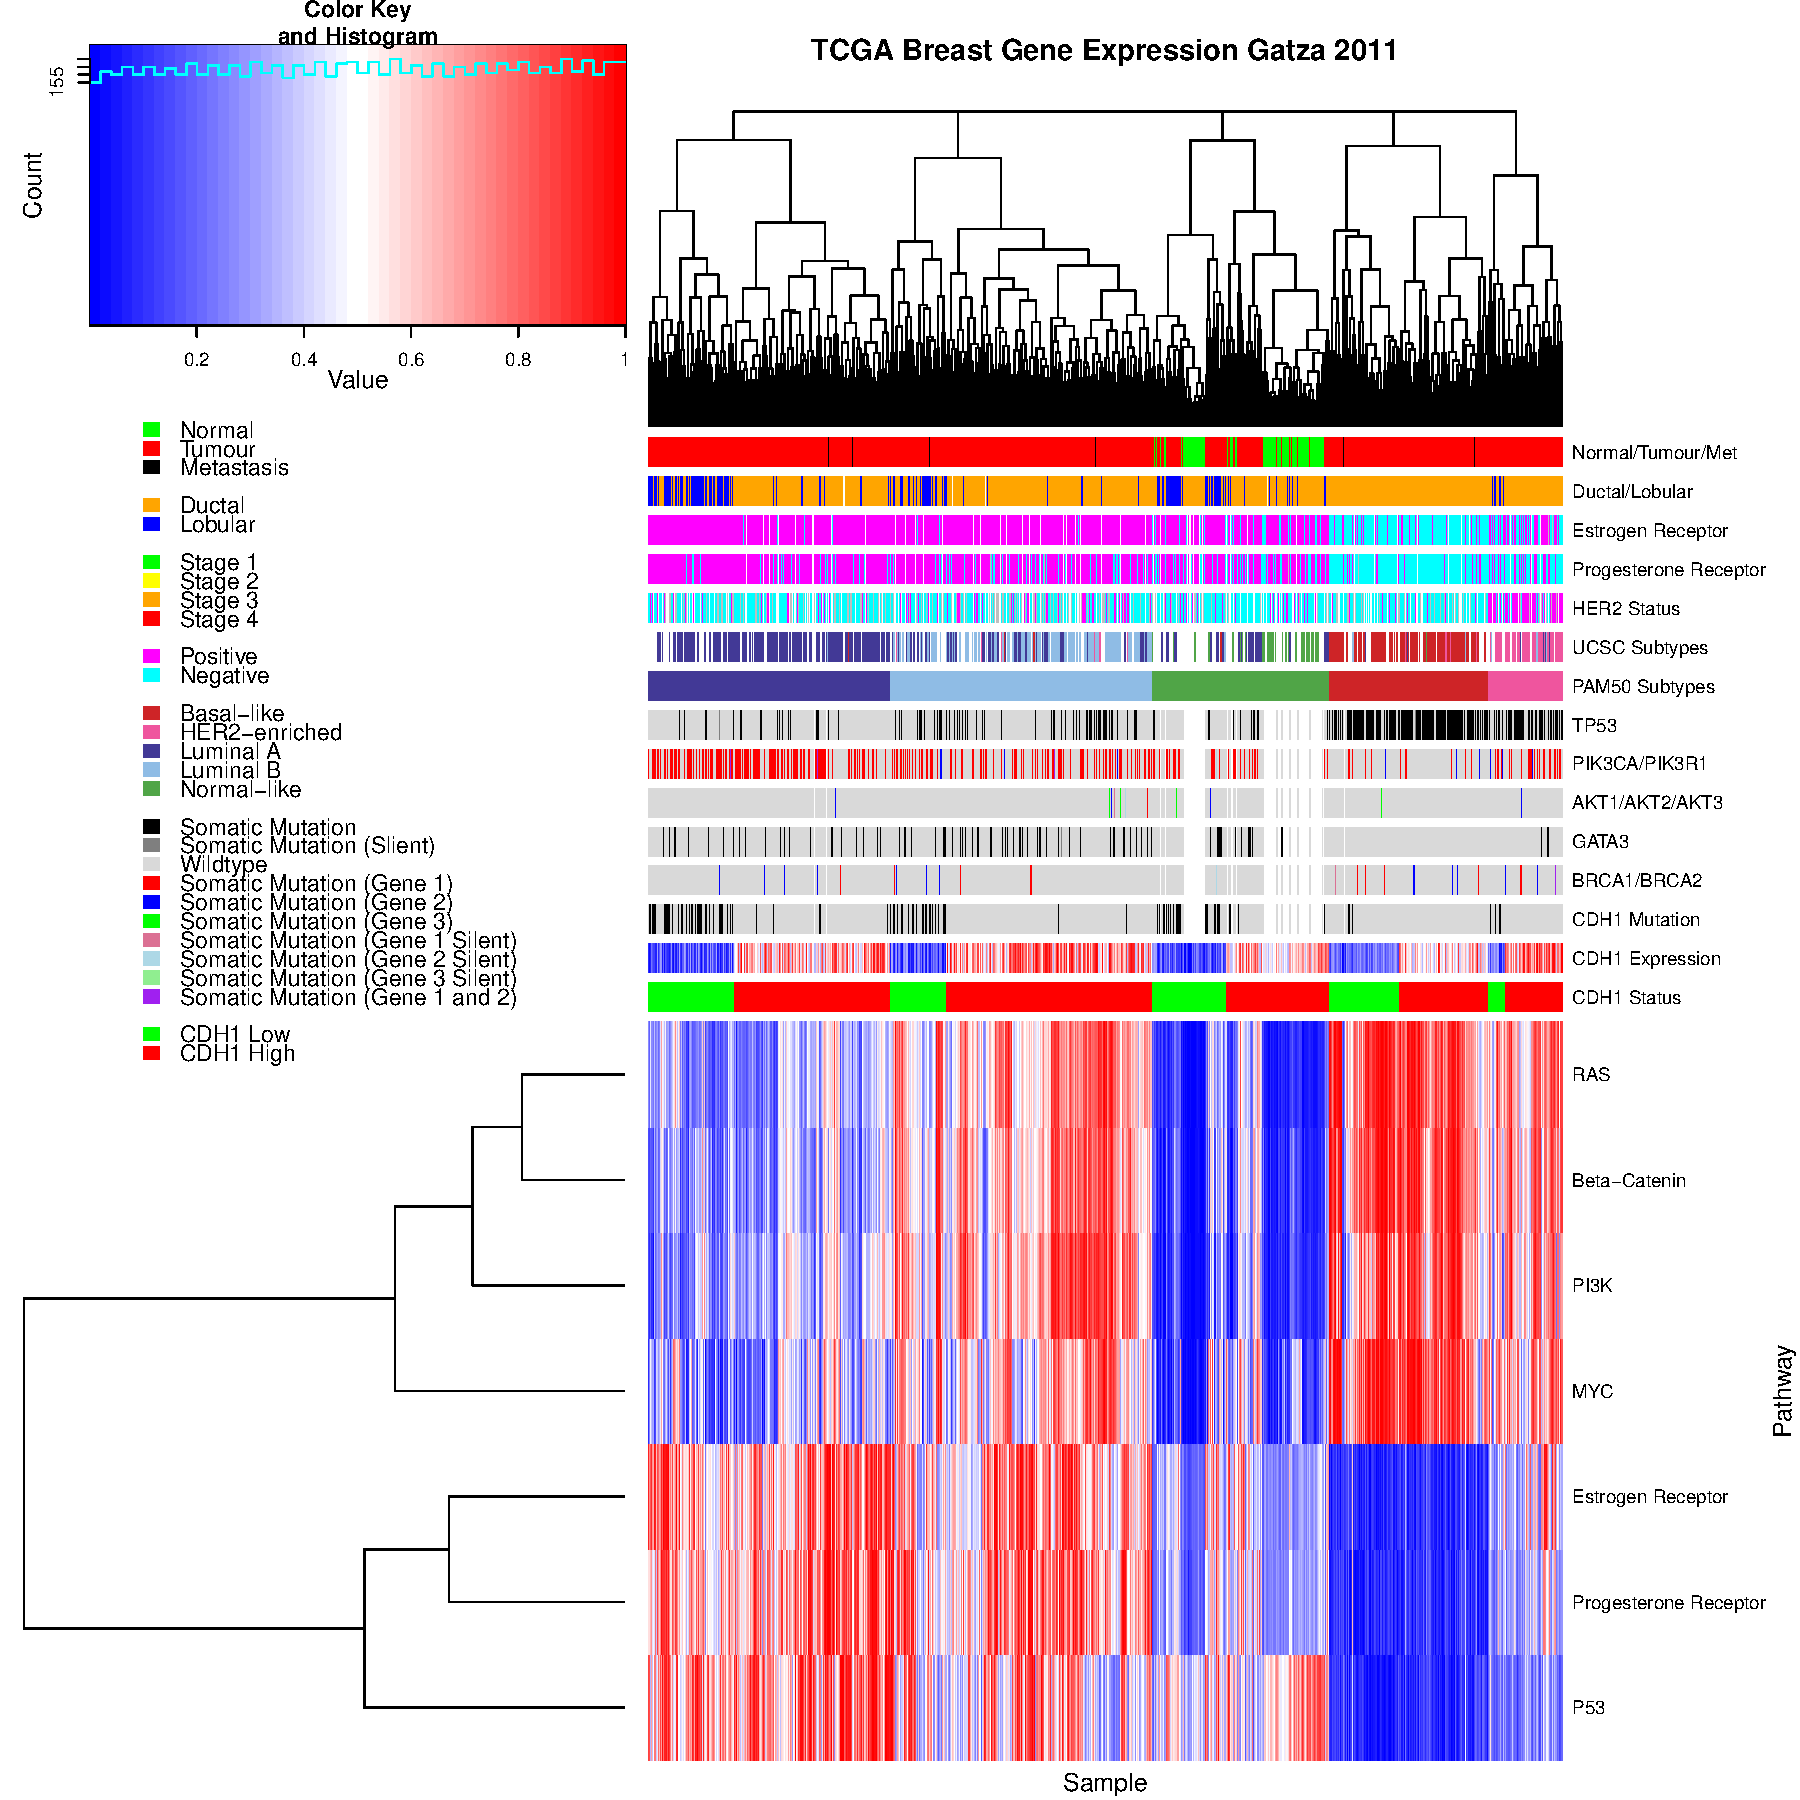
\includegraphics{CDH1_Heatmaps_Gatza2011(ranked)_Full_split_by_Subtype_and_CDH1_Stat_corr2.pdf} %original pdf, png for edited %1.png = Gatza 2011, 2.png = Cropped, 3.png = excl. PI3K
   }
   \end{center}
   \caption[Pathway meta\gls{gene expression} profiles]{\small \textbf{Pathway meta\gls{gene expression} profiles.} Expression profiles for \gls{metagene} signatures from \citet{Gatza2011} in \gls{TCGA} breast data, annotated for clinical factors (with sample types and histological results coloured according to the legend) and cancer gene \glspl{mutation} (Negative values for \gls{mutation} are light grey with missing data in white). \Glspl{intrinsic subtype} are shown as derived from \gls{microarray} (\gls{UCSC}) and \gls{RNA-Seq} (\gls{PAM50}) data \citep{TCGA2012, Parker2009}. Samples were clustered independently for each \glspl{intrinsic subtype} and by \textit{CDH1} \glslink{gene expression}{expression} status. Pathway \glslink{gene expression}{expression} signatures are consistent with \glspl{mutation} and clinical subgroups.
}
\label{fig:metagene_expr_Gatza2011}
\end{minipage}
%} %close fbox
} %close centering
\end{figure*}

These gene signatures reflect \glspl{intrinsic subtype}s as expected. In particular, the estrogen and progesterone receptor signatures are low in the predominantly \gls{ER}$^-$ and \gls{PR}$^-$ basal-like subtype tumours. These tumours also had the highest frequency of \textit{TP53} \glspl{mutation} and a corresponding reduction of p53 \gls{metagene} activity, as expected for loss of a \gls{tumour suppressor}. The luminal A and luminal B tumour subtypes are the most similar, which is reflected in these \glspl{metagene} signatures, although they are distinguishable molecular subtypes as shown by elevated \gls{PI3K}, AKT, RAS, and $\beta$-catenin signalling in luminal B tumours. However, these pathways were also elevated in basal-like and HER2-enriched subtypes and lowly expressed in the ``normal-like'' subtype (which contained the normal samples). These \glspl{intrinsic subtype} specific gene signature profiles were further supported with \glspl{metagene} for an extended set of signatures \citep{Gatza2014}, as shown in Figure~\ref{fig:metagene_expr_Gatza2014}.

\textit{TP53} \glspl{mutation} were the most frequent and more common in the basal-like subtype. Similarly, \textit{GATA3} \glspl{mutation} were more common in luminal subtype tumours. \gls{PI3K} \glspl{mutation} were more frequent across breast tumours, although these were less common in the basal-like subtype despite an elevated \gls{metagene} (this discrepancy will the discussed further in Section~\ref{chapt3:metagene_mut}). \textit{CDH1} \glspl{mutation} similarly occurred across molecular subtypes with the exception of the basal-like subtype (as observed in \gls{gene expression} with Figure~\ref{fig:slipt_expr}). \textit{CDH1} low samples occurred in all subtypes but were predominantly of the lobular histological ubtype. Apart from these genes, \glspl{mutation} did not show clear specificity to a particular subtype and the variation between samples reflects the range of molecular cascades that can result in tumours with similar molecular profiles, supporting the use of \gls{gene expression} data for cancer diagnostics and identification of molecular targets. 

The direction of each \gls{metagene} was consistent with the clinical characteristics, which formed a consensus of gene activity as shown for the \gls{PI3K} and \gls{ER} signatures \citep{Gatza2011} in Figures~\ref{fig:metagene_expr_Gatza2011_PI3K} and~\ref{fig:metagene_expr_Gatza2011_ER}, respectively.  Supporting data for p53 and BRCA \glspl{metagene} \citep{Gatza2011, Gatza2014} are given in the Appendix (Figures~\ref{fig:metagene_expr_Gatza2011_P53} and~\ref{fig:metagene_expr_Gatza2014_BRCA}). In each of the examples for gene signatures% for PI3K (Figure~\ref{fig:metagene_expr_Gatza2011_PI3K}), p53 (Figure~\ref{fig:metagene_expr_Gatza2011_P53}), estrogen receptor (Figure~\ref{fig:metagene_expr_Gatza2011_ER}), and BRCA (Figure~\ref{fig:metagene_expr_Gatza2014_BRCA}) genes \citep{Gatza2011, Gatza2014}
, the \glslink{gene expression}{expression} of the majority of the genes were highly concordant with the \gls{metagene}, being either positively or negatively correlated. These were generally consistent with established clinical and molecular subtypes of breast cancer and the \glspl{recurrent mutation} shown. However, the \textit{PIK3CA} and \textit{PIK3R1} \gls{mutant} samples did not necessarily have elevated \gls{PI3K} pathway \gls{metagene} activity (as shown in Figure~\ref{fig:metagene_expr_Gatza2011_PI3K}).  


\begin{figure*}[!htp]
\noindent\makebox[\textwidth][c]{%               %centering
%\noindent\fbox{
\begin{minipage}{1.15 \textwidth}  %frame beyond textwidth
\begin{center}
  \resizebox{1 \textwidth}{!}{
    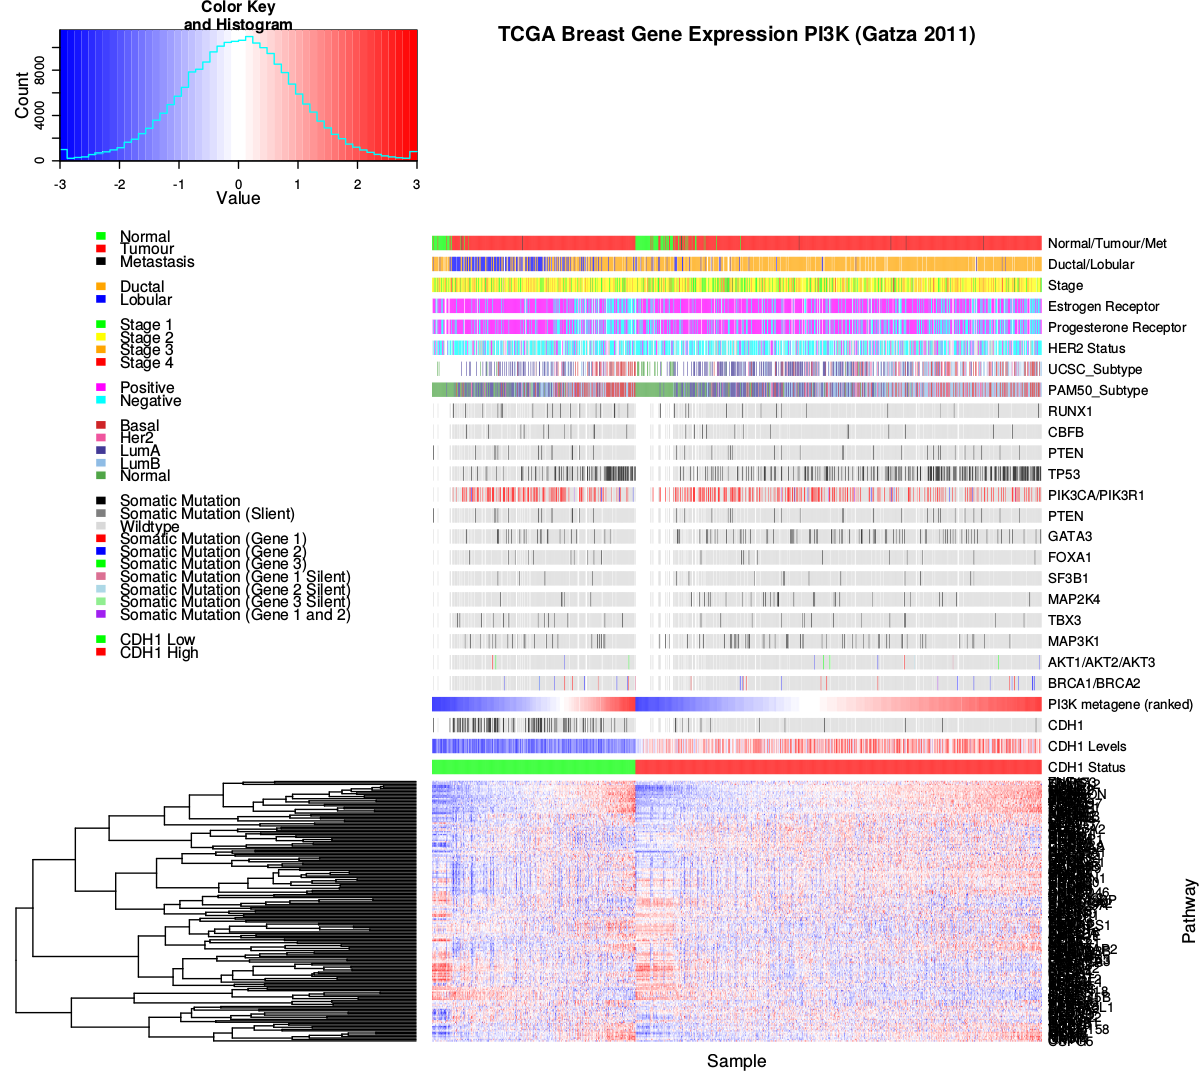
\includegraphics{CDH1_Heatmaps_Gatza2011(PI3K)_Full_Metagene_mgorder.png} %original pdf, png for edited
   }
   \end{center}
   \caption[Expression profiles for constituent genes of PI3K]{\small \textbf{Expression profiles for constituent genes of PI3K.} Expression profiles the genes contained in the \gls{PI3K} gene signature from \citet{Gatza2011} in \gls{TCGA} breast data, annotated for clinical factors and cancer gene \glspl{mutation}. Samples are separated by \textit{CDH1} \glslink{gene expression}{expression} status and sorted by the \gls{metagene}. In both cases, the majority of genes were consistent with the direction of the \gls{PI3K} \gls{metagene}, although considerable proportion were inversely correlated with the \gls{metagene}. Normal samples had low \gls{PI3K} meta\gls{gene expression} and \textit{TP53} \gls{mutant} samples had high \gls{PI3K} \glslink{gene expression}{expression}. Although, oncogenic \textit{PIK3CA} and \gls{tumour suppressor} \textit{PIK3R1} \glspl{mutation} across samples including those with low \gls{metagene} response.
}
\label{fig:metagene_expr_Gatza2011_PI3K}
\end{minipage}
%} %close fbox
} %close centering
\end{figure*}

\begin{figure*}[!htp]
\noindent\makebox[\textwidth][c]{%               %centering
%\noindent\fbox{
\begin{minipage}{1.15 \textwidth}  %frame beyond textwidth
\begin{center}
  \resizebox{1 \textwidth}{!}{
    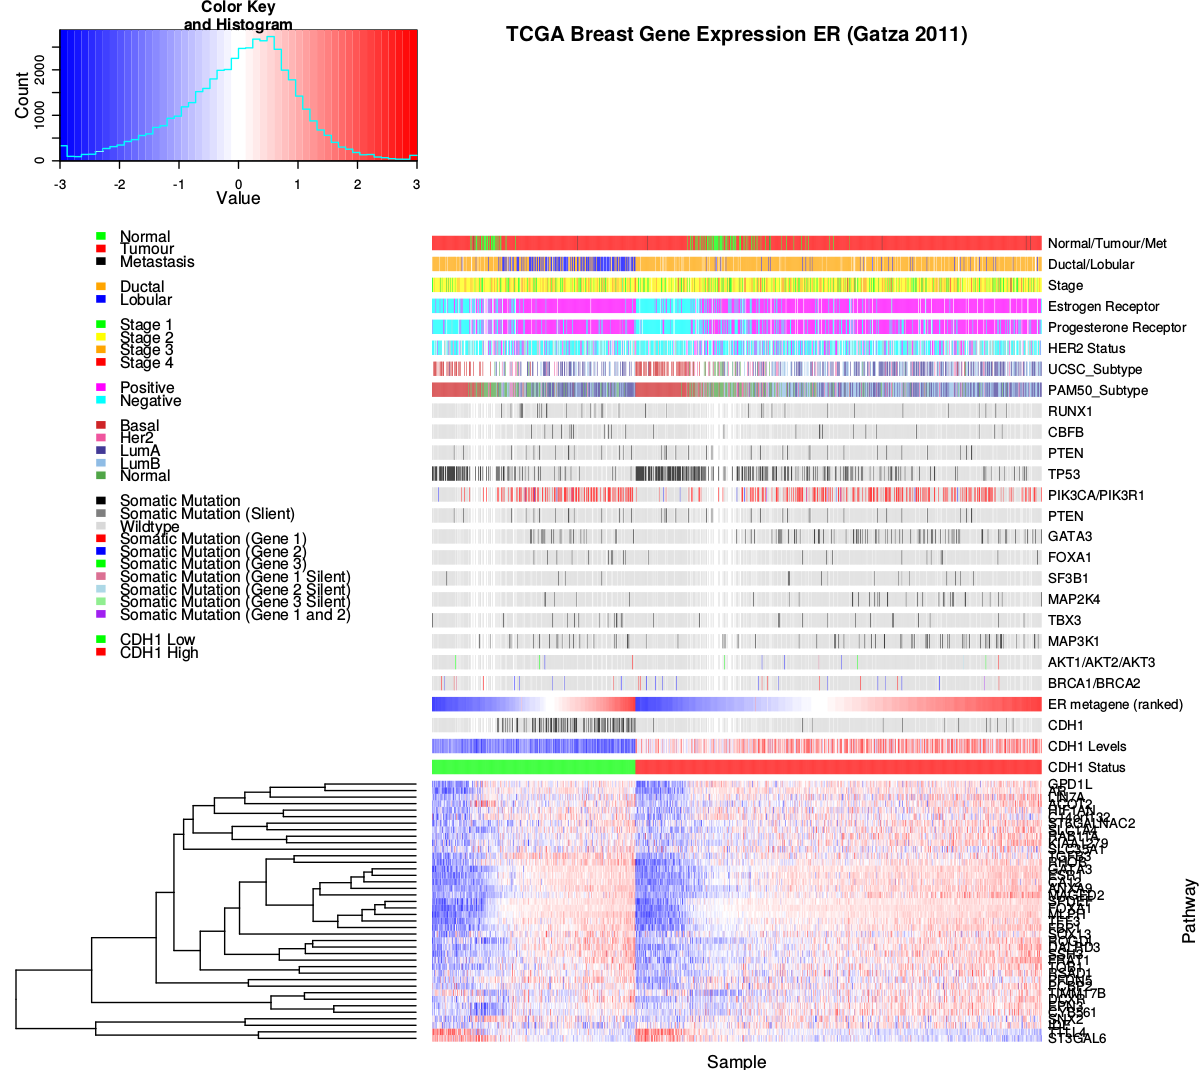
\includegraphics{CDH1_Heatmaps_Gatza2011(ER)_Full_Metagene_mgorder.png} %original pdf, png for edited
   }
   \end{center}
   \caption[Expression profiles for estrogen receptor related genes]{\small \textbf{Expression profiles for estrogen receptor related genes.} Expression profiles the genes contained in the estrogen receptor (ER) gene signature from \citet{Gatza2011} in \gls{TCGA} breast data, annotated for clinical factors and cancer gene \glspl{mutation}. Samples are separated by \textit{CDH1} \glslink{gene expression}{expression} status and sorted by the \gls{metagene}. In both cases, the majority of genes were consistent with the direction of the \gls{metagene}, with very few exceptions being inversely correlated. Estrogen receptor (by antibody staining) negative samples had low  meta\gls{gene expression}, as expected. These were more likely to be ductal and basal subtypes, lacking \textit{CDH1} or \textit{PIK3CA} \glspl{mutation}.
}
\label{fig:metagene_expr_Gatza2011_ER}
\end{minipage}
%} %close fbox
} %close centering
\end{figure*}


%\FloatBarrier

\subsection{Somatic Mutation}  \label{chapt3:metagene_mut}



\begin{figure*}[!ht]
%\begin{mdframed}
        \begin{center}
%
        \subcaptionbox{\textit{PIK3CA}}{%
           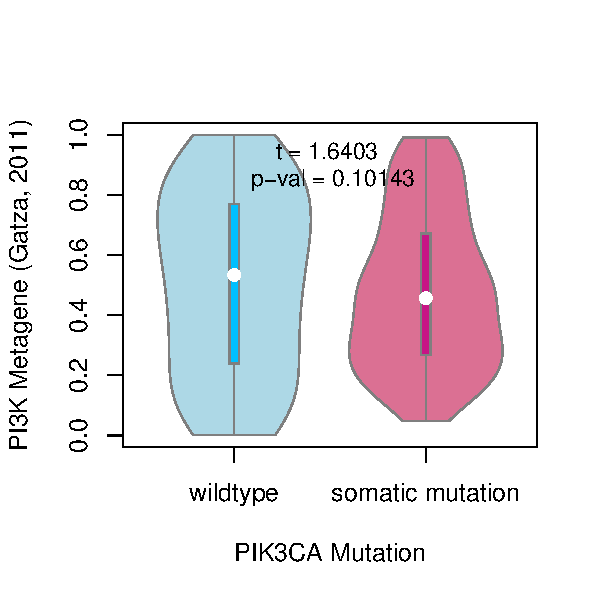
\includegraphics[width=0.35\textwidth]{metagene(ranked)_vioplotx_Mutation_PI3K2011_PIK3CA.pdf}
        }%
        \subcaptionbox{\textit{PIK3CA} or \textit{PIK3R1}}{%
           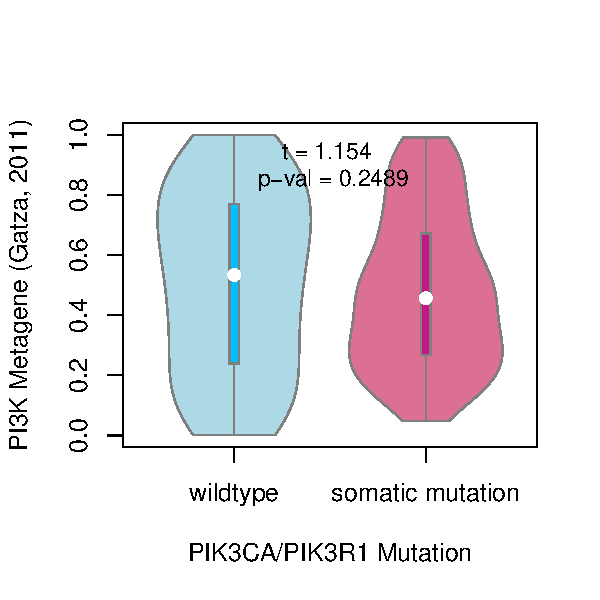
\includegraphics[width=0.35\textwidth]{metagene(ranked)_vioplotx_Mutation_PI3K2011_PIK3CA_PIK3R1.pdf}
        }
        
        \subcaptionbox{\textit{CDH1}}{%
           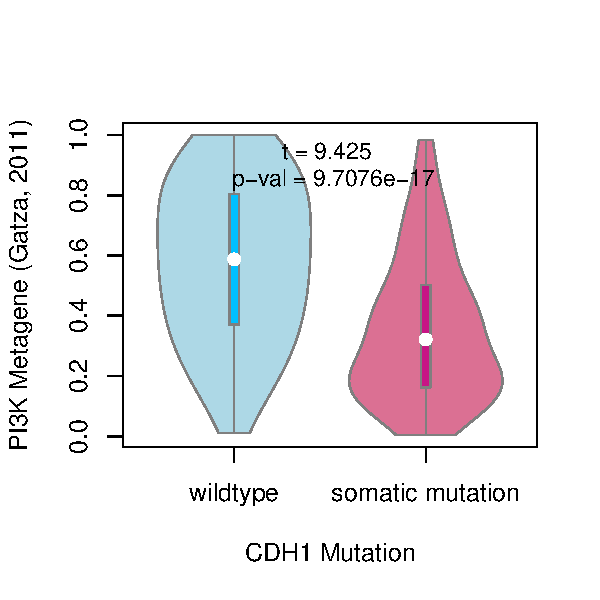
\includegraphics[width=0.35\textwidth]{metagene(ranked)_vioplotx_Mutation_PI3K2011_CDH1.pdf}
        }%
        \subcaptionbox{\textit{TP53}}{%
           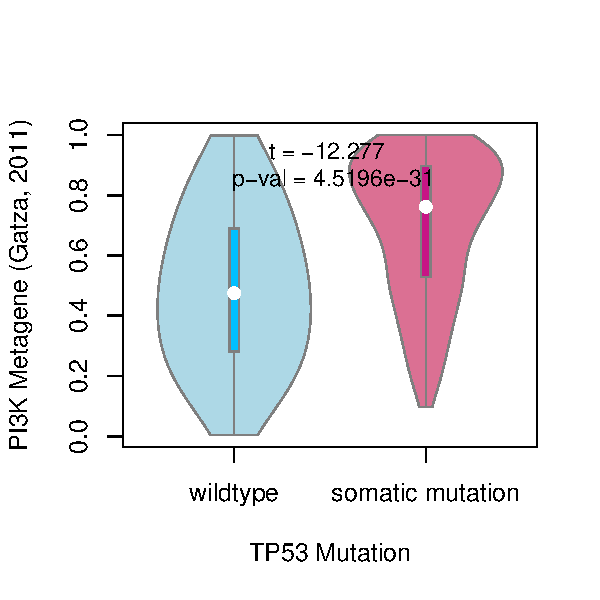
\includegraphics[width=0.35\textwidth]{metagene(ranked)_vioplotx_Mutation_PI3K2011_TP53.pdf}
        }
    \end{center}
    \caption[Somatic \gls{mutation} against the PI3K \gls{metagene}]{\small \textbf{Somatic \gls{mutation} against the \gls{PI3K} \gls{metagene}.} Mutations in \textit{PIK3CA}, \textit{PIK3R1}, \textit{CDH1}, and \textit{TP53} were examined in \gls{TCGA} breast cancer for their association with the \gls{PI3K} \citep{Gatza2011} pathway \gls{metagene}. The \glspl{tumour suppressor} \textit{CDH1} and \textit{TP53} showed an increase and decrease in the \gls{metagene} respectively, whereas \textit{PIK3CA} and \textit{PIK3R1} \glspl{mutation} had little effect on the \gls{metagene} levels.
}
\label{fig:mutation_expr_mg}
%\end{mdframed}
\end{figure*}

It should be noted that \glspl{metagene}, while consistent with the consensus of constituent expressed genes, were not necessarily reflecting the \glslink{somatic}{somatic} \gls{mutation} status. The \gls{PI3K} \citep{Gatza2011} \gls{metagene} levels in particular, were not statistically significantly varying between \gls{mutant} and\gls{wild-type} \textit{PIK3CA} samples (shown in Figure~\ref{fig:mutation_expr_mg}). However, the \gls{PI3K} \gls{metagene} differed across \textit{CDH1} and \textit{TP53} \glspl{mutation}, remarkably in opposite directions considering that \gls{PI3K} is an oncogenic growth pathway and these are both most frequently \glspl{tumour suppressor} inactivated in cancers. This shows that \textit{CDH1} and \textit{TP53} deficient tumours have distinct molecular growth pathways and that \gls{synthetic lethal} interventions against loss of \textit{CDH1} function may not be applicable to other cancers with \glspl{driver mutation} such as \textit{TP53}, although these were kept in the analysis for comparison. These differences may be related to these \glspl{mutation} being more frequent in tumours with difference clinical characteristics (as observed in Section~\ref{chapt3:metagene_expression}).  Thus \glspl{mutation} do not necessarily have corresponding changes in pathway \glslink{gene expression}{expression}, particularly for \glspl{oncogene} which may change in function rather than being upregulated.


While the more specific \textit{PIK3CA} \citep{Gatza2014} \gls{metagene} showed significant differences with \textit{PIK3CA} and \textit{PIK3R1} \glspl{mutation} (as shown in Figure~\ref{fig:mutation_expr_mg2}), this \gls{metagene} replicated stronger differences for \textit{CDH1} and \textit{TP53}.  These differences were less pronounced in the protein levels of p110$\alpha$ (enocded by \textit{PIK3CA}) and the downstream AKT gene (shown in Figures~\ref{fig:mutation_expr_prot} and~\ref{fig:mutation_expr_prot2} respectively). However, this may be due to this regulatory cascade (kinases) being transmitted as a change in protein state (phosphorylation) rather than changes in \glslink{gene expression}{expression} levels. Another consideration is that \glspl{mutation} at different loci have different effects on protein function, particularly for \glspl{oncogene}.

\FloatBarrier

\iffalse
\subsection{Mutation locus}  \label{chapt3:metagene_mut_locus}

The gene locus distribution of \textit{PIK3CA} and its receptor \textit{PIK3R1} were consistent with oncogenic and \gls{tumour suppressor} \glspl{mutation}, as shown in Figure~\ref{fig:mutation_locus}. \textit{PIK3CA} has \glspl{recurrent mutation} in 2 hotspots, centered around the E545K and H1047R (shown in Figure~\ref{fig:mutation_locus:PIK3CA}), as expected for an \gls{oncogene}. This contrasts with the \glspl{tumour suppressor}, \textit{PIK3R1}, and \textit{CDH1} (shown in Figures~\ref{fig:mutation_locus:PIK3R1} and~\ref{fig:mutation_locus:CDH1} respectively), which have low frequency inactivating \glspl{mutation} spread across them. A notable exception is \textit{TP53} (shown in Figure~\ref{fig:mutation_locus:TP53}) which displays both inactivating \glspl{mutation} throughout and recurrent (oncogenic) \glspl{mutation} at high frequency, consistent with the complex role of \textit{TP53} in cancer biology which is outside of the scope of this thesis and shown for comparison. 


\begin{figure*}[!ht]
%\begin{mdframed}
        \begin{center}
%
        \subcaptionbox{\textit{PI3KCA} gene}{%
            %\label{fig:simulate_function:first}
            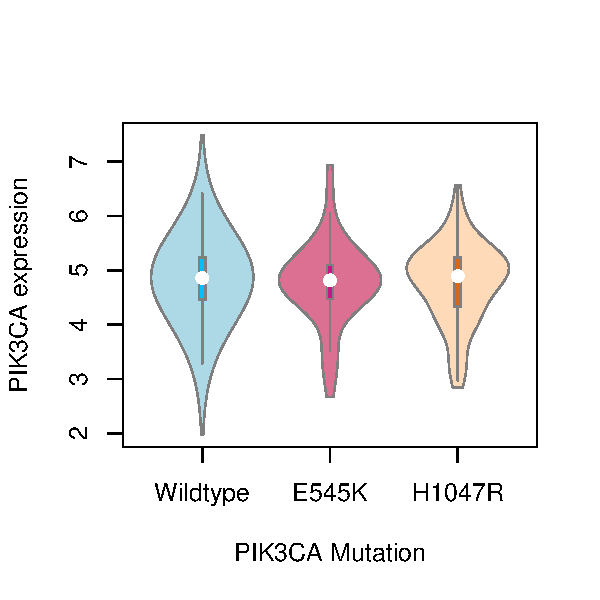
\includegraphics[width=0.3\textwidth]{geneexpr_vioplotx_Mutation_locus_PIK3CA.pdf}
        }%
        \subcaptionbox{\textit{PI3KCA} \gls{metagene}}{%
            %\label{fig:simulate_function:first}
            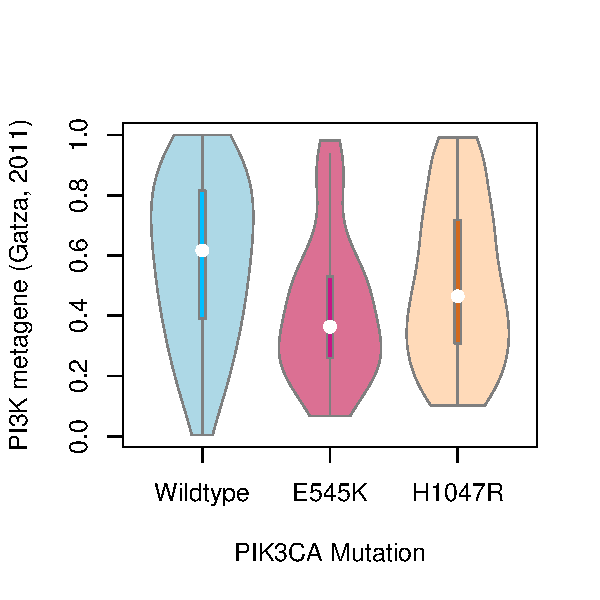
\includegraphics[width=0.3\textwidth]{metagene_vioplotx_Mutation_locus_PIK3CA.pdf}
        }%
        \subcaptionbox{\textit{PIK3R1} gene}{%
           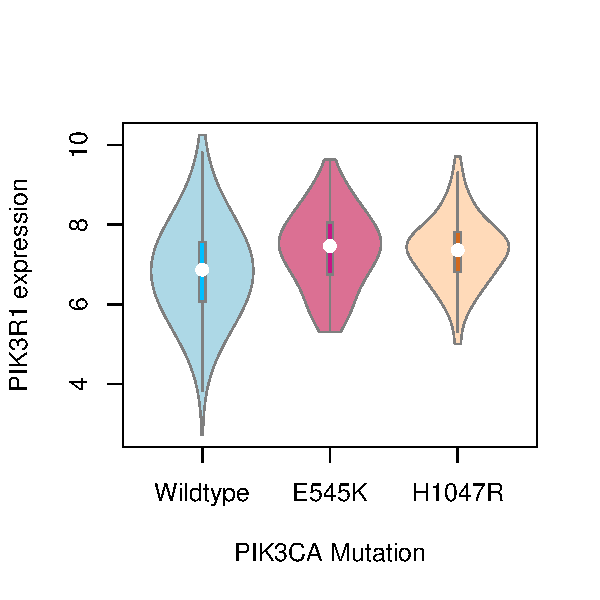
\includegraphics[width=0.3\textwidth]{geneexpr_vioplotx_Mutation_locus_PIK3R1.pdf}
        }
        
        \subcaptionbox{\textit{PIK3CA} protein}{%
           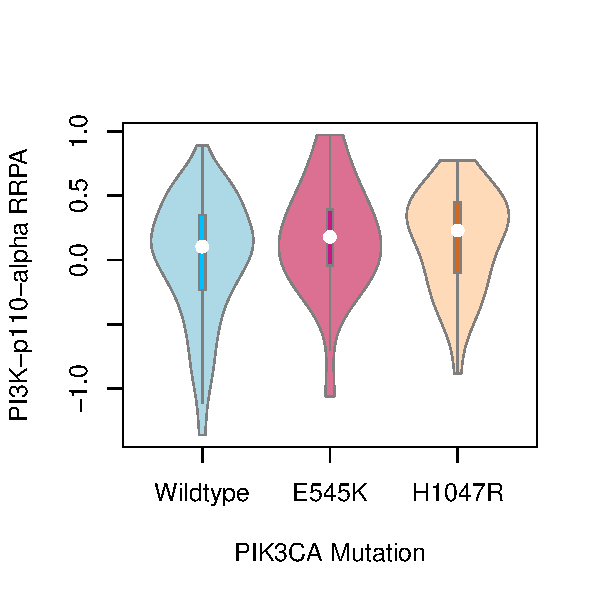
\includegraphics[width=0.3\textwidth]{protein_vioplotx_Mutation_locus_PIK3CA.pdf}
        }%
        \subcaptionbox{\textit{AKT} protein}{%
           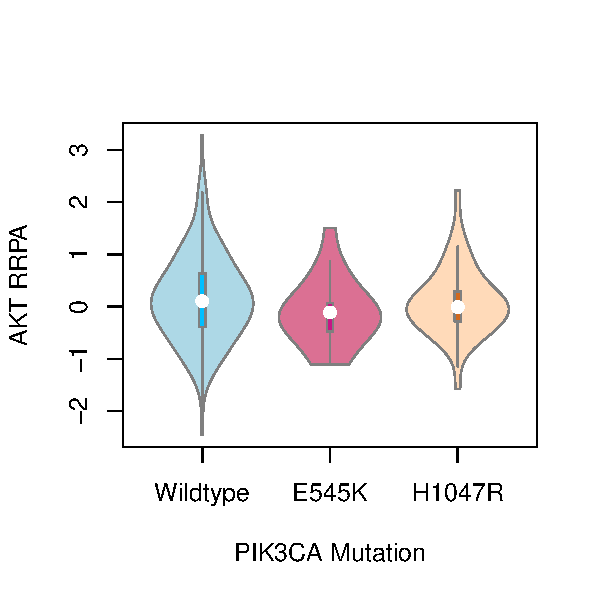
\includegraphics[width=0.3\textwidth]{protein_vioplotx_Mutation_locus_AKT.pdf}
        }
        
        \subcaptionbox{\textit{CDH1} protein}{%
           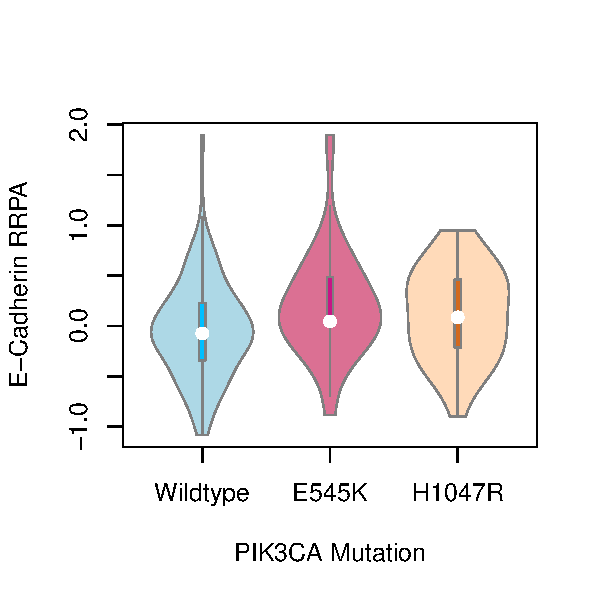
\includegraphics[width=0.3\textwidth]{protein_vioplotx_Mutation_locus_CDH1.pdf}
        }%
        \subcaptionbox{\textit{TP53} protein}{%
           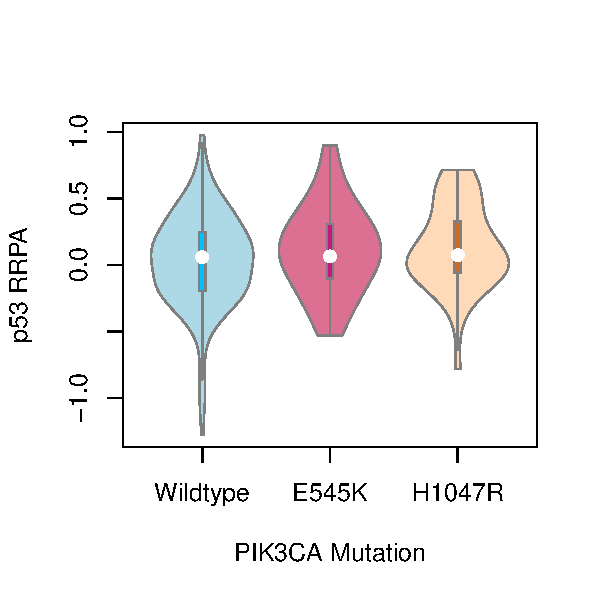
\includegraphics[width=0.3\textwidth]{protein_vioplotx_Mutation_locus_TP53.pdf}
        }
    \end{center}
    \caption[Somatic \gls{mutation} locus against \glslink{gene expression}{expression}]{\small \textbf{Somatic \gls{mutation} locus against \glslink{gene expression}{expression}.} The recurrent E545K and H1047R \gls{oncogene} \glspl{mutation} in \textit{PIK3CA} were examined in \gls{TCGA} breast cancer to show the effect of \gls{mutation} locus on gene, pathway, and protein \glslink{gene expression}{expression}. While neither of these \glspl{mutation} had an impact of \textit{PIK3CA} \acrshort{mRNA} \glslink{gene expression}{expression}, E545K had specifically lower PI3K \citep{Gatza2011} \gls{metagene} levels and both \glspl{mutation} had higher \textit{PIK3R1} \acrshort{mRNA} \glslink{gene expression}{expression}. However, these differences were not reflected in the protein \glslink{gene expression}{expression} levels.
}
\label{fig:mutation_expr}
%\end{mdframed}
\end{figure*}

These differences in gene locus may explain why \glspl{mutation} do not necessarily have corresponding changes in gene or meta\gls{gene expression}. Specfically, the recurrent E545K and H1047R \gls{oncogene} \glspl{mutation} in \textit{PIK3CA} did not affect \textit{PIK3CA} \acrshort{mRNA} \glslink{gene expression}{expression} but E545K had specifically lower PI3K \citep{Gatza2011} \gls{metagene} levels. Both \glspl{mutation} had higher \textit{PIK3R1} \acrshort{mRNA} \glslink{gene expression}{expression} but these differences differences were not reflected in the protein \glslink{gene expression}{expression} levels of p110$\alpha$ protein (encoded by \textit{PIK3CA}), its downstream target AKT, \gls{E-cadherin} (encoded by \text{CDH1}), or p53 (as ashown in Figure~\ref{fig:mutation_expr}).

While the complex effects of \gls{mutation} in \glspl{oncogene} such as \textit{PIK3CA} are not necessarily detected in a pathway \gls{metagene}, these do capture the consensus of pathway \gls{gene expression} and account for other potential means of pathway activation. Thus \glspl{metagene} are sufficient as a measure of gene activity for the purposes of \gls{synthetic lethal} detection with \gls{SLIPT}. This approach is more applicable to \gls{tumour suppressor} genes with a relationship between \gls{gene expression} and activity (rather than activation at the protein level) but this is not a major concern since \glspl{synthetic lethal} is more clinically relevant for targeting \gls{tumour suppressor} \glspl{mutation} than \glspl{oncogene}.
\fi


\FloatBarrier

\subsection{Synthetic Lethal Pathway Metagenes} \label{chapt3:metagene_SL}

Pathway \glspl{metagene} for Reactome pathways (generated as described in Section~\ref{methods:metagene}) were also used for testing \gls{synthetic lethal} partner pathways with \textit{CDH1} by \gls{SLIPT}. Since the \glspl{metagene} have are higher when the pathway as a whole is activated, they are amenable to \gls{SLIPT} analysis using low \gls{metagene} levels for inactivated pathways. These \gls{synthetic lethal} \glspl{metagene} differed to the over-represented pathways among \gls{synthetic lethal} gene candidates. However, there were some similarities to previous findings, as shown in Tables~\ref{tab:metagene_SL}. In particular, translational pathways were replicated as observed in Table~\ref{tab:pathway_exprSL}. While the specific pathways differ, immune pathways (e.g., NF-$\kappa$B) were also supported by \gls{metagene} \gls{synthetic lethal} analysis.

\begin{table*}[!ht]
\caption{Candidate \gls{synthetic lethal} \glspl{metagene} against \textit{CDH1} from SLIPT}
\label{tab:metagene_SL}
\centering
\resizebox{1 \textwidth}{!}{
\begin{threeparttable}
\begin{tabular}{sl^l^c^c^c^c^c}
\rowstyle{\bfseries}
 Pathway & ID & Observed & Expected & $\chi^2$value & p-value & p-value (\gls{FDR}) \\ 
  \hline
  \rowcolor{black!10}
  Glycogen storage diseases & 3229121 & 68 & 130 & 176 & $6.62 \times 10^{-37}$ & $1.82 \times 10^{-34}$ \\ 
  \rowcolor{black!5}
  Myoclonic epilepsy of Lafora & 3785653 & 68 & 130 & 176 & $6.62 \times 10^{-37}$ & $1.82 \times 10^{-34}$ \\ 
  \rowcolor{black!10}
  Diseases of carbohydrate metabolism & 5663084 & 68 & 130 & 176 & $6.62 \times 10^{-37}$ & $1.82 \times 10^{-34}$ \\ 
  \rowcolor{black!5}
  Arachidonic acid metabolism & 2142753 & 81 & 130 & 157 & $8.13 \times 10^{-33}$ & $1.49 \times 10^{-30}$ \\ 
  \rowcolor{black!10}
  Translation initiation complex formation & 72649 & 70 & 130 & 152 & $7.08 \times 10^{-32}$ & $1.17 \times 10^{-29}$ \\ 
  \rowcolor{black!5}
  Synthesis of 5-eicosatetraenoic acids & 2142688 & 68 & 130 & 151 & $1.25 \times 10^{-31}$ & $1.88 \times 10^{-29}$ \\ 
  \rowcolor{black!10}
  SRP-dependent cotranslational protein targeting to membrane & 1799339 & 69 & 130 & 150 & $2.01 \times 10^{-31}$ & $2.76 \times 10^{-29}$ \\ 
  \rowcolor{black!5}
  L13a-mediated translational silencing of Ceruloplasmin \glslink{gene expression}{expression} & 156827 & 72 & 130 & 148 & $5.91 \times 10^{-31}$ & $6.44 \times 10^{-29}$ \\ 
  \rowcolor{black!10}
  3' -UTR-mediated translational regulation & 157279 & 72 & 130 & 148 & $5.91 \times 10^{-31}$ & $6.44 \times 10^{-29}$ \\ 
  \rowcolor{black!5}
  \begin{tabular}[c]{@{}l@{}}Activation of the \acrshort{mRNA} upon binding of the cap-binding complex and eIFs,\\and subsequent binding to 43S \end{tabular} & 72662 & 70 & 130 & 147 & $1.14 \times 10^{-30}$ & $9.28 \times 10^{-29}$ \\ 
  \rowcolor{black!10}
  Formation of the ternary complex, and subsequently, the 43S complex & 72695 & 70 & 130 & 147 & $1.14 \times 10^{-30}$ & $9.28 \times 10^{-29}$ \\ 
  \rowcolor{black!5}
  Ribosomal scanning and start codon recognition & 72702 & 70 & 130 & 147 & $1.14 \times 10^{-30}$ & $9.28 \times 10^{-29}$ \\ 
  \rowcolor{black!10}
  Eukaryotic Translation Elongation & 156842 & 72 & 130 & 146 & $1.19 \times 10^{-30}$ & $9.28 \times 10^{-29}$ \\ 
  \rowcolor{black!5}
  Nonsense Mediated Decay independent of the Exon Junction Complex & 975956 & 71 & 130 & 146 & $1.24 \times 10^{-30}$ & $9.28 \times 10^{-29}$ \\ 
  \rowcolor{black!10}
  Viral \acrshort{mRNA} Translation & 192823 & 70 & 130 & 146 & $1.51 \times 10^{-30}$ & $1.04 \times 10^{-28}$ \\ 
  \rowcolor{black!5}
  Eukaryotic Translation Termination & 72764 & 70 & 130 & 146 & $1.51 \times 10^{-30}$ & $1.04 \times 10^{-28}$ \\ 
  \rowcolor{black!10}
  NF-kB is activated and signals survival & 209560 & 71 & 130 & 145 & $1.90 \times 10^{-30}$ & $1.19 \times 10^{-28}$ \\ 
  \rowcolor{black!5}
  Peptide chain elongation & 156902 & 72 & 130 & 145 & $1.91 \times 10^{-30}$ & $1.19 \times 10^{-28}$ \\ 
  \rowcolor{black!10}
  Influenza Life Cycle & 168255 & 70 & 130 & 145 & $1.95 \times 10^{-30}$ & $1.19 \times 10^{-28}$ \\ 
  \rowcolor{black!5}
  Formation of a pool of free 40S subunits & 72689 & 73 & 130 & 145 & $2.01 \times 10^{-30}$ & $1.19 \times 10^{-28}$ \\ 
  \rowcolor{black!10}
  Nonsense-Mediated Decay & 927802 & 71 & 130 & 145 & $2.44 \times 10^{-30}$ & $1.34 \times 10^{-28}$ \\ 
  \rowcolor{black!5}
  Nonsense Mediated Decay enhanced by the Exon Junction Complex & 975957 & 71 & 130 & 145 & $2.44 \times 10^{-30}$ & $1.34 \times 10^{-28}$ \\ 
  \rowcolor{black!10}
  GTP hydrolysis and joining of the 60S ribosomal subunit & 72706 & 72 & 130 & 145 & $2.58 \times 10^{-30}$ & $1.37 \times 10^{-28}$ \\ 
  \rowcolor{black!5}
  Influenza Viral \acrshort{RNA} Transcription and Replication & 168273 & 72 & 130 & 144 & $4.01 \times 10^{-30}$ & $2.07 \times 10^{-28}$ \\ 
  \rowcolor{black!10}
  Signalling by NOTCH1 HD Domain Mutants in Cancer & 2691230 & 79 & 130 & 143 & $5.99 \times 10^{-30}$ & $2.82 \times 10^{-28}$ \\ 
  \hline
\end{tabular}
\begin{tablenotes}
\raggedright \small
Strongest candidate \gls{synthetic lethal} partners for \textit{CDH1} by \gls{SLIPT} with observed and expected numbers of \gls{TCGA} breast cancer samples with low \glslink{gene expression}{expression} of both \textit{CDH1} and the \gls{metagene}.
\end{tablenotes}
\end{threeparttable}
}
\end{table*}

Signalling pathways were more strongly supported by \acrshort{mtSLIPT} analysis of \gls{metagene} pathway \glslink{gene expression}{expression} against \textit{CDH1} \gls{mutation}, as shown in Table~\ref{tab:metagene_mtSL}, although these results were generally less statistically significant than \glslink{gene expression}{expression} analyses. Signalling pathways detected as \gls{synthetic lethal} \glspl{metagene} include G$_{\alpha z}$, insulin-related growth factor (IGF), GABA receptor, G$_{\alpha s}$, S6K1 and various toxin responses mediated by \glspl{GPCR}. Metabolic processes including processing of carbohydrates and fatty acids were also implicated across these analyses.

The \gls{metagene} analyses differ more between expresssion and \textit{CDH1} \gls{mutation} than previous analyses, with more specific signalling pathways identified in the \gls{mutation} analysis. This supports the usage of a complete null \gls{mutant} model in experimental testing for \glspl{synthetic lethal} of signalling pathways against \text{CDH1} inactivation rather than a knockdown in \glslink{gene expression}{expression}. However, low \glslink{gene expression}{expression} of partners has been used in either case to be applicable to dose-dependent pharmacological inhibition and across genes where \glspl{mutation} have different functional consequences, including variants of unknown significance. 

These results show an independent pathway-based approach to detecting \gls{synthetic lethal} gene functions interacting with \textit{CDH1}. The use of \gls{synthetic lethal} \glspl{metagene} replicates support for these pathways independent of pathway size (as genes are weighted equally). Along with the verifying that the direction of \glspl{metagene} recapitulates the activity of a pathway, these demonstrate that many of the pathways previously identified from over-represent\-ed \gls{synthetic lethal} genes (detected by \gls{SLIPT}) are \gls{synthetic lethal} pathways with their activity dependent on \gls{synthetic lethal} genes rather than containing \gls{synthetic lethal} genes as inhibitors or peripheral regulators of the pathways.

\subsection{Synthetic Lethality in Breast Cancer}

The \gls{synthetic lethal} analysis against low \textit{CDH1} \glslink{gene expression}{expression} supports prior findings in translational and immune pathways even if they were not able to detected in an experimental screen \citep{Telford2015}. Together these findings support the role of \textit{CDH1} loss in cancer disrupting cell signalling with wider effects on protein translation and metabolism necessary for the proliferation of cancer cells. This is consistent with the \gls{GPCR} pathways such as G$_{\alpha s}$ signalling being supported by \gls{SLIPT} gene candidates and the experimental primary \gls{siRNA} screen, as shown by resampling in Section~\ref{chapt3:compare_pathway_perm}.

%%appendix
%\label{tab:metagene_mtSL}

\FloatBarrier

%\section{Synthetic Lethality by Somatic Mutation}

%\section{Mutation analysis}
%Data in Appendix~\ref{appendix:mutation_analysis} %%discussed above

\iffalse
\subsection{ANOVA of Expression Predictors}
[include?]

Another approach was to only use copy number, \gls{mutation}, or hyper-methylation data for genes in which they would impact on gene function and occur frequently in tumours. Before investigating whether these impact on gene function, they were investigated as predictors of variation in \gls{gene expression}. If these are not giving variation independent of \gls{gene expression}, \glslink{gene expression}{expression} would be a more suitable measure of gene function as it is widely generated in studies and useful as a clinical biomarker.

Globally predicting \gls{gene expression} across all genes from \acrshort{DNA} copy number and \glslink{somatic}{somatic} \gls{mutation} was attempted by \gls{ANOVA}. However, this was computationally challenging and gene-specific analyses would be more informative. Gene specific \gls{ANOVA} and linear regression was performed but was raised more issues than it addressed. There were issues with interaction terms and \gls{mutation} data, many genes were not tested for these since there were so few \glspl{mutation} for these genes in the dataset.  It was possible to include \acrshort{DNA} methylation in gene-specific analyses (despite the concerns raised above) but the $R^2$ values for each gene were still generally very low and issues with insufficient \gls{mutant} samples for interaction terms became worse. This means that the approach used differs for each gene making it difficult to compare them. The challenges raised here suggested that \glslink{gene expression}{expression} is very difficult to predict with other factors but including these other factors would be difficult and plagued by multiple-testing, particularly comparing between them with the current \gls{synthetic lethal} prediction method. This led to investigations into the simulation of \glspl{synthetic lethal}.
\fi

\FloatBarrier

\section{Replication in Stomach Cancer} \label{chapt3:stad_replication}

\textit{CDH1} is also important in stomach cancer biology as a \glslink{driver mutation}{driver} \gls{tumour suppressor} gene, including as a \gls{germline} \gls{mutation} in many cases of \gls{hereditary} diffuse gastric cancer. The \gls{synthetic lethal} analysis of genes and pathways (previously identified for \gls{TCGA} breast cancer data) was replicated in \gls{TCGA} stomach cancer. The accompanying data for \gls{SLIPT} analysis against \textit{CDH1} \glslink{gene expression}{expression} is provided in Appendix~\ref{appendix:stad_exprSL}.

While the sample size was lower for \gls{TCGA} stomach cancer (particularly for \glspl{mutation}), these results serve to support the findings in breast cancer in an independent patient cohort and tissue samples. The molecular profiling, including \gls{RNA-Seq} \glslink{gene expression}{expression}, were performed by \gls{TCGA} using the sample procedures as for breast cancer and the findings reported here were performed used data analysis techniques identical to those presented previously. These procedures should ensure as close comparison as feasible across cancer types for those relevant to \gls{HDGC} and recurrent \textit{CDH1} \glspl{mutation}.

The strongest \gls{SLIPT} genes for stomach cancer (shown in Table~\ref{tab:gene_stad_SL}) did not necessarily directly correspond to those observed in breast cancer (shown in Table~\ref{tab:gene_SL}). However, several gene functions were replicated in stomach cancer. Together, these gene candidates indicate widespread functions of \textit{CDH1} and strongly detectable \glspl{synthetic lethal} with many genes from a strategy that can be applied across cancer types. More specifically, the signalling genes included \gls{GPCR} signalling genes, which was one of the most supported \gls{synthetic lethal} pathways in breast cancer analysis, the experimental screen \citep{Telford2015}.%, and has many actionable drug targets which have been applied to other diseases.
These findings were further supported by the pathways over-represented in \gls{SLIPT} candidates from \gls{TCGA} stomach cancer (shown in Table~\ref{tab:pathway_stad_exprSL}) which replicated the translational and immune pathways observed in \gls{TCGA} breast cancer (shown in Table~\ref{tab:pathway_exprSL}) and further supported GCPR signalling pathways, including the class A/1 receptors. The extracellular matrix was also detected at the pathway level in stomach cancer, including elastic fibres, glycosylation, collagen, and integrin cell-surface interactions. 
While fewer pathways were supported by resampling for the intersection of \gls{SLIPT} and experimental screen \citep{Telford2015} candidate partners in stomach cancer than breast cancer, many of those detected (shown in Table~\ref{tab:pathway_perm_overlap_stad}) replicate those detected in breast cancer (shown in Table~\ref{tab:pathway_perm_overlap}). The pathways detected by both permutation and over-representation were more likely to be replicated across stomach and breast cancer than those detected by over-representation alone, supporting the use of this procedure to detect \gls{synthetic lethal} pathways applicable across cancer types. The include G$_{\alpha s}$ signalling and elastic fibre formation as discussed for breast cancer (in Section~\ref{chapt3:compare_pathway_perm}).

\iffalse
\subsection{Synthetic Lethal Genes and Pathways} \label{chapt3:stad_SL_genes}

The strongest \gls{SLIPT} genes for stomach cancer (shown in Table~\ref{tab:gene_stad_SL}) did not necessarily directly correspond to those observed in breast cancer (shown in Table~\ref{tab:gene_SL}). However, several gene functions were replicated in stomach cancer. Cell membrane genes including \textit{EMP3}, \textit{GYPC},  \textit{LGALS1}, \textit{PRR24},  and \textit{FUNCD2} were among the strongest SL candidates. Similarly, cell signalling genes including \textit{PLEKHO1}, \textit{RARRES2}, \textit{VEGFB}, \textit{HSPB2}, and \textit{CREM} were detected in stomach cancers. It is notable that several of these genes (\textit{EMP3}, \textit{PLEKHO1}, and \textit{FUNCD2}) have a known role in cancer. Together these genes support the roles of \textit{CDH1} in cell membrane and signalling functions (of epithelial tissues) which are perturbed in both breast and stomach cancers.

The strongest \acrshort{mtSLIPT} genes tested against \textit{CDH1} mutatoin for stomach cancer (shown in Table~\ref{tab:gene_stad_mtSL}) supported similar gene functions. Membrane and cell-adhesion genes including \textit{KFBP6},\textit{THY1},\textit{CLELC2B}, \textit{NISCH}, \textit{TSPAN1},and \textit{KCTD12} and signalling genes including \textit{ZEB2}, \textit{CCND2}, \textit{NEURL1B}, \textit{KFBP6}, and \textit{OGN} were detected. Similarly, these include cancer genes such as \textit{VIM},\textit{ZEB2},\textit{BCL2},\textit{THY1}, and \textit{RUNX1T1}. The \acrshort{mtSLIPT} procedure also replicated several of the strongest candidates in breast cancer (shown in Table~\ref{tab:gene_mtSL}) such as \textit{NRIP2} and \textit{NISCH}.

Together, these gene candidates indicate widespread functions of \textit{CDH1} and strongly detectable \glspl{synthetic lethal} with many genes from a strategy that can be applied across cancer types. More specifically, the signalling genes included \gls{GPCR} signalling genes (e.g., \textit{GNG11}, \textit{GNAI1}, \textit{DZIP1}, \textit{PTGFR}, and \textit{KCTD12}), a growth signalling pathway which was one of the most supported \gls{synthetic lethal} pathways in breast cancer analysis, the experimental screen \citep{Telford2015}, and has many actionable drug targets which have been applied to other diseases.

These findings were further supported by the pathways over-represented in \gls{SLIPT} candidates from \gls{TCGA} stomach cancer (shown in Table~\ref{tab:pathway_stad_exprSL}) which were replicated the translational and immune pathways observed in \gls{TCGA} breast cancer (shown in Tabel~\ref{tab:pathway_exprSL}). Further support for GCPR signalling pathways including the class A/1 receptors. The extracellular matrix was also detected at the pathway level in stomach cancer \gls{SLIPT} candidates and replicated in \acrshort{mtSLIPT} analysis for \textit{CDH1} \gls{mutation} (shown in Table~\ref{tab:pathway_stad_mtSL}), including elastic fibres, glycosylation, collagen, and integrin cell-surface interactions. Thus there was strong evidence for the role of extracellular matrix pathways and the tumour microenvironment in \textit{CDH1} deficient stomach cancers, in addition to cell signalling and translation pathways important in tumour growth across breast and stomach cancer.




%%appendix

\FloatBarrier

\subsection{Synthetic Lethal Expression Profiles} \label{chapt3:stad_SL_clusters}

%The \glslink{gene expression}{expression} profiles of candidate \gls{synthetic lethal} partners dtected by \gls{SLIPT} and \acrshort{mtSLIPT} in stomach cancer were plotted against clinical characteristics as described for breast cancer data in Section~\ref{chapt3:exprSL_clusters} (shown in Figures~\ref{fig:slipt_expr_stad} and~\ref{fig:slipt_expr_stad_mtSL} respectively). As expected the majority of \textit{CDH1} \gls{mutant} samples had low \glslink{gene expression}{expression} of \textit{CDH1} and were the diffuse type of stomach cancer.


\begin{figure*}[!ht]
%\begin{mdframed}
  \centering
  \resizebox{0.99 \textwidth}{!}{
    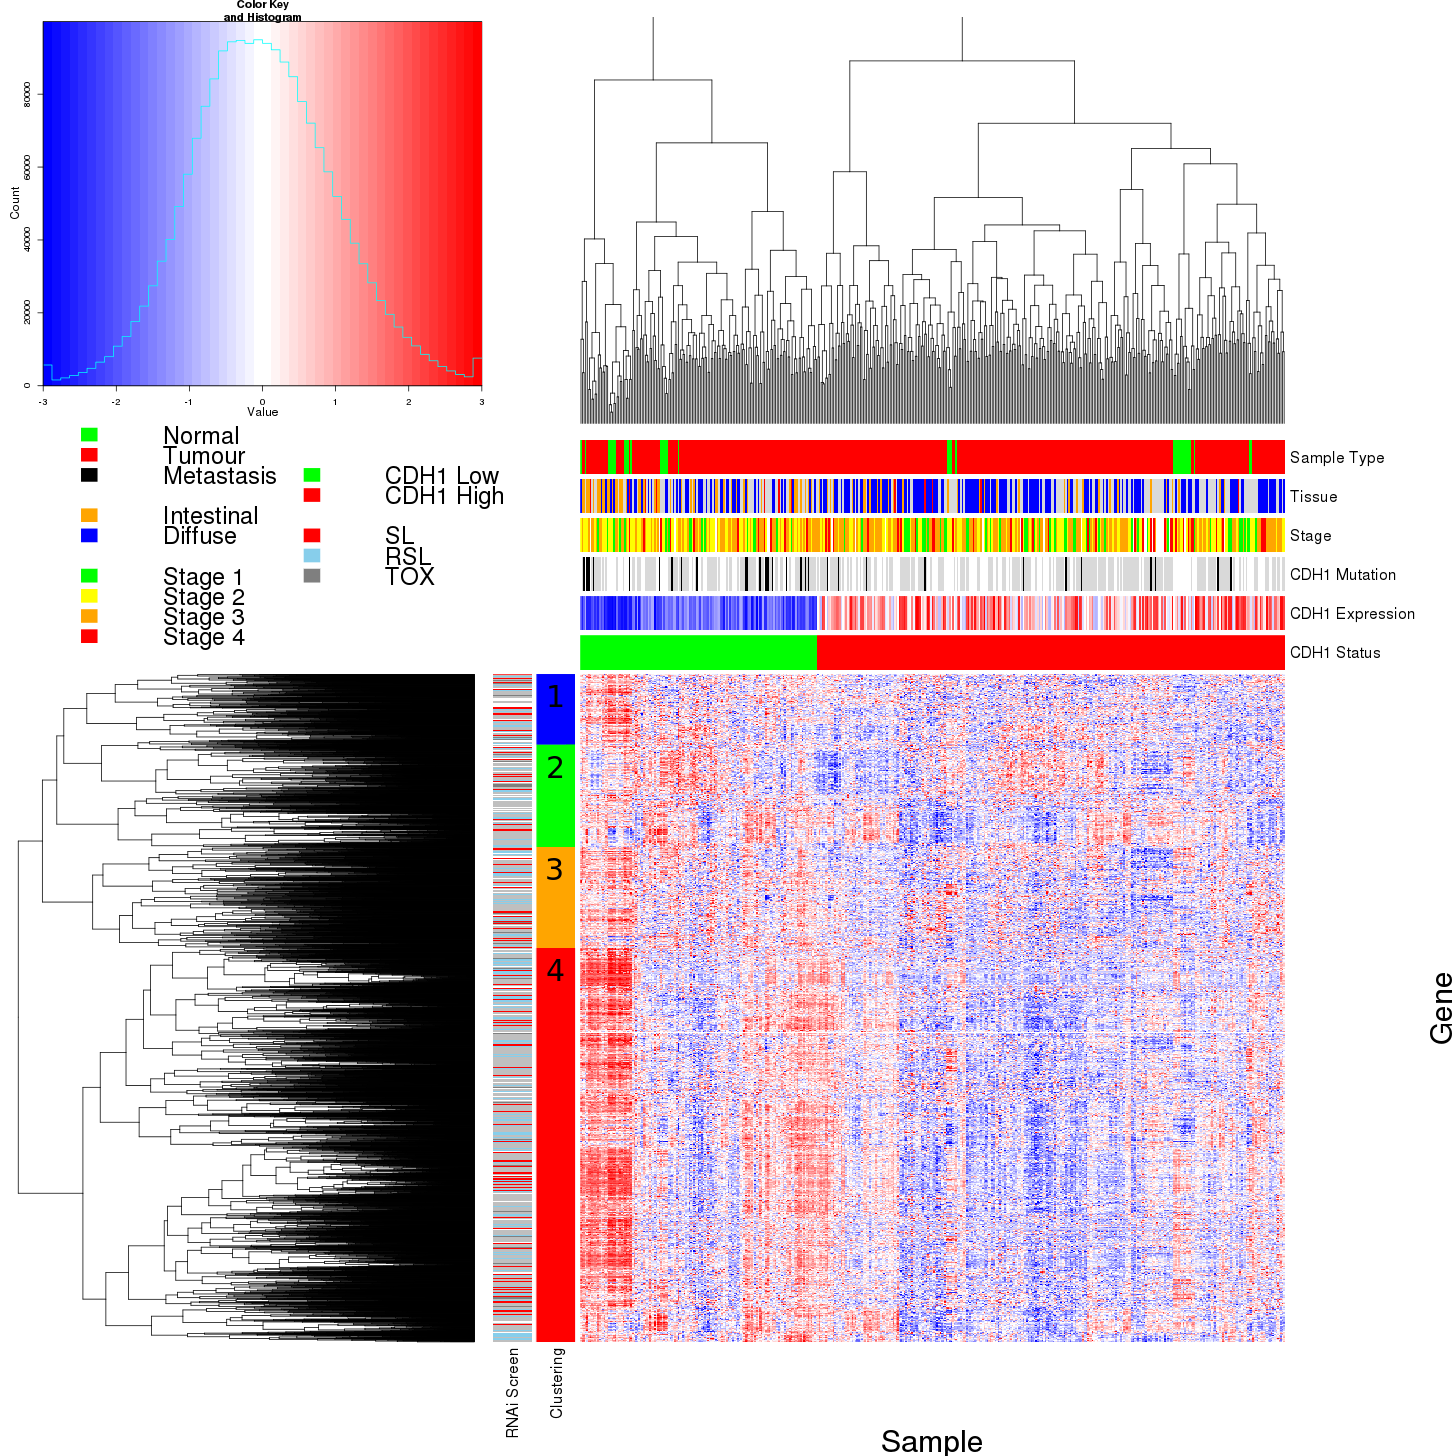
\includegraphics{CDH1_Heatmaps_Genes_Split_By_CDH1_z-trans_exprSL_cordistx_Pub_stad.png}
   }
    \caption[Synthetic lethal \glslink{gene expression}{expression} profiles of stomach samples]{\small \textbf{Synthetic lethal \glslink{gene expression}{expression} profiles of analysed samples.} \Gls{gene expression} profile heatmap (correlation distance) of all samples (separated by the $\sfrac{1}{3}$ quantile of \textit{CDH1} \glslink{gene expression}{expression}) analysed in \gls{TCGA} stomach cancer dataset for \gls{gene expression} of 4365 candidate partners of \gls{E-cadherin} (\textit{CDH1}) from \gls{SLIPT} prediction (with significant \gls{FDR} adjusted $p < 0.05$). Deeply clustered, inter-correlated genes form several main groups, each containing genes that were SL candidates or toxic in an \gls{siRNA} screen \cite{Telford2015}. Clusters had different sample groups highly expressing the \gls{synthetic lethal} candidates in \textit{CDH1} low samples, notably diffuse and \textit{CDH1} \gls{mutant} samples have elevated \glslink{gene expression}{expression} in one or more distinct clusters, although there was less complexity and variation among candidate \gls{synthetic lethal} partners than in breast data. \textit{CDH1} low samples also contained most of samples with \textit{CDH1} \glspl{mutation}.
   %This suggests that multiple targets may be needed to target \textit{CDH1} deficiency across genetic backgrounds and that combination therapy may be more effective. 
}
\label{fig:slipt_expr_stad}
%\end{mdframed}
\end{figure*}

%The \gls{SLIPT} partners of \textit{CDH1} exhibited similar clustering in staomch cancer to breast cancer, replicating the diverse roles of elevated partner genes in different clinical samples. Specifically (in Figure~\ref{fig:slipt_expr_stad}), the diffuse type stomach cancers had higher \glslink{gene expression}{expression} of the candidate \gls{synthetic lethal} partners (where \textit{CDH1} has a role as a \gls{driver mutation}), despite an unbiased clustering. This is consistent with compensating \glslink{gene expression}{expression} of \gls{synthetic lethal} partners under loss of \textit{CDH1}, as suggested by \citet{Lu2015}. The pathway composition of gene clusters for stomach cancer (shown in Table~\ref{tab:pathway_clusters_stad}) was also highly concordant with breast cancer findings (shown in Table~\ref{tab:pathway_clusters}). These included replicated of translation (Cluster 1), immune functions (Cluster 2), G$_{\alpha s}$ signalling (Cluster 3), and further support for the roles of \glspl{GPCR} and the extracellular matrix (Cluster 4) in the \gls{synthetic lethal} partners and functions of \textit{CDH1}, replicated across stomach and breast cancers. Clusters 1 and 4, which had particularly high \glslink{gene expression}{expression} of \gls{SLIPT} candidate partner genes in the diffuse subtype, also had the most significant over-representation of pathways.

%There was less variation between the \glslink{gene expression}{expression} profiles of \acrshort{mtSLIPT} partners of \textit{CDH1} in stomach cancer, although clusters were still detectable (as shown in Figure~\ref{fig:slipt_expr_stad_mtSL}). While the genes and pathways detected was lewss significant (due to lower sample size), the composition of clusters was further indicative for the roles of extracellular matrix (including elastic fibres), immune functions, and the cell signalling.

\FloatBarrier

\subsection{Comparison to Primary Screen} \label{chapt3:compare_SL_genes_stad}

The number of genes detected by both \gls{SLIPT} in \gls{TCGA} stomach cancer data and \gls{siRNA} in breast cell lines (shown in Figure~\ref{fig:Venn_allgenes_stad}) was also not a significant overlap (as observed for breast cancer in Figure~\ref{fig:Venn_allgenes}). This was particularly the case of \acrshort{mtSLIPT} against \textit{CDH1} \gls{mutation} in stomach cancer which detected very few genes (as shown in Figure~\ref{fig:Venn_allgenes_stad_mtSL}) due to low sample size and \gls{mutation} frequency.

This smaller overlap can also be attributed to the tissue-specific differences between the stomach cancers and the breast cells used for the experimental model \citep{Chen2014}. Nevertheless, many genes were detected across \gls{SLIPT} in stomach cancers and the experimental screen \citep{Telford2015} and the pathways detected were consistent with prior observations in breast cancer. Despite differences in the specific genes detected, the functions of \textit{CDH1} were conserved across epithetial cancers in different tissues and \gls{synthetic lethal} inhibition of interacting pathways may be effective against molecular targets such as \textit{CDH1} inactivation across tissue types.

However, the pathway composition of \gls{SLIPT}-specific genes and those replicated with the \gls{siRNA} primary screen \citep{Telford2015} were highly concordant between the pathways identified by \gls{SLIPT} in \gls{TCGA} stomach cancer (shown in Table~\ref{tab:Venn_over-representation_stad}) and pathways previously identified in \gls{TCGA} breast cancer (shown in Table~\ref{tab:Venn_over-representation}). In both cases, translation and immune pathways were highly over-represented in \gls{SLIPT}-specific genes, which we would not expect to be detected by \gls{siRNA} screening in cell lines, as discussed in Section~\ref{chapt3:compare_pathway}. In addition, the extracellular matrix was supported by in stomach cancer. While the pathways identified by specifically by \gls{SLIPT} in stomach cancer or \gls{siRNA} screening were similar to those observed for breast cancer (in Table~\ref{tab:Venn_over-representation}), the pathways over-represented in the intersection for stomach cancer \gls{SLIPT} candidates and the \gls{siRNA} primary screen \citep{Telford2015} also had a clear over-representation of signalling pathways, although they differed from those observed in breast cancer \gls{SLIPT} candidates. \gls{GPCR} signalling was supported in genes detected in both \gls{TCGA} stomach cancer and screening, including G$_{\alpha q}$, G$_{\alpha s}$, serotonin receptors, and class A signalling (shown in more detail in Table~\ref{tab:pathway_perm_overlap_stad}). In addition MAPK and NOTCH signalling pathways were detected. These replicate the findings in breast cancer and show consistent detection of signalling pathways in stomach cancer despite less genes being detected by \gls{SLIPT} and patient samples differing from the tissue in which the experiments were conducted.

Similarly, the \gls{SLIPT}-specific gene candidates against \textit{CDH1} \gls{mutation} (shown in Table~\ref{tab:Venn_over-representation_stad_mtSL}) replicated pathways observed in breast cancer (shown in Table~\ref{tab:Venn_over-representation_mtSL}), despite a lower number of genes detected. In particular, the extracellular matrix and elastic fibres were over-represented. While the number of genes overlapping with the \gls{siRNA} was too low to be amenable to pathway analysis, there is further indication that members of these genes replicated across \gls{mutation} \gls{SLIPT} analyses include cell-membrane, elastic fibre, and \gls{GPCR} signalling genes. 

\FloatBarrier

\subsubsection{Resampling Analysis}  \label{chapt3:compare_pathway_perm_stad_SL}

Similarly, resampling for \gls{SLIPT} specific candidates (shown in Tables~\ref{tab:pathway_perm_stad} and~\ref{tab:pathway_perm_stad_mtSL}) replicated many of the most highly over-represented pathways in stomach cancer. These include translational, immune, \gls{GPCR} signalling, and elastic fibres, consistent with previous analyses in breast cancer (shown in Tables~\ref{tab:pathway_perm} and~\ref{tab:pathway_perm_mtSL}).

While fewer pathways were supported by resampling for the intersection of \gls{SLIPT} and experimental screen \citep{Telford2015} candidate partners in stomach cancer than breast cancer, many of those detected (shown in Table~\ref{tab:pathway_perm_overlap_stad}) replicate those detected in breast cancer (shown in Tables~\ref{tab:pathway_perm_overlap} and~\ref{tab:pathway_perm_overlap_mtSL}). The pathways detected by both permutation and over-representation were more likely to be replicated across stomach and breast cancer than those detected by over-representation alone, supporting the use of this procedure to detect \gls{synthetic lethal} pathways applicable across cancer types. The include G$_{\alpha s}$ signalling and elastic fibre formation as discussed for breast cancer (in Section~\ref{chapt3:compare_pathway_perm}).

While many pathways were detected by resampling for \acrshort{mtSLIPT} against \textit{CDH1} \gls{mutation} in stomach cancer (shown in Table~\ref{tab:pathway_perm_overlap_stad_mtSL}), there were not enough genes detected by both \acrshort{mtSLIPT} and the \gls{siRNA} primary screen to determine over-represented pathways. Therefore this may be due to small numbers of genes which does not constitute support for pathway composition. However, this under-powered analysis does not preclude the replicated \gls{synthetic lethal} pathways detected across \gls{SLIPT} \glslink{gene expression}{expression} analyses in \gls{TCGA} breast and stomach cancer data with an accompanying \gls{siRNA} primary screen \citep{Telford2015}. Rather this further supports the use of \gls{SLIPT} to test against low \glslink{gene expression}{expression} of query genes as measure of gene inactivation to avoid this issue, despite \gls{mutation} (which often produces similar results) being more indicative of complete gene inactivation.

\FloatBarrier

\subsection{Metagene Analysis} \label{chapt3:metagene_stad_SL}

\Gls{metagene} analysis (as conducted in Section~\ref{chapt3:metagene_SL}) was also performed for \gls{TCGA} stomach cancer \glslink{gene expression}{expression} data, using Reactome pathways. These results (as shown in Table~\ref{tab:metagene_stad_SL}) provided further support for signalling and extracellular processes as \gls{synthetic lethal} pathways across stomach and breast cancer. Namely, cell-cell communication, VEGF signalling, and various \gls{GPCR} pathways were detected.  

Signalling and immune pathways were also supported by \acrshort{mtSLIPT} analysis of \gls{metagene} pathway \glslink{gene expression}{expression} against \textit{CDH1} \gls{mutation}, as shown in Table~\ref{tab:metagene_stad_mtSL}. However, these results were generally less statistically significant than \glslink{gene expression}{expression} analyses. Signalling pathways detected as \gls{synthetic lethal} \glspl{metagene} include prostacyclin, SCF-KIT, ERK, MAPK, NGF, VEGF, and PI3K/AKT. The innate immune response, the inflammasome, and integrin signalling were also implicated to be \gls{synthetic lethal} with \textit{CDH1 \glspl{mutation}}. Cell surface interactions, cholesterol biosynthesis, and platelet homeostasis also support the role of extracellular processes in proliferation of \textit{CDH1} deficient cancers and interactions of \textit{CDH1} with the extracellular environment that was not tested in the cell line experimental screen.

%%appendix
%\label{tab:metagene_stad_mtSL}
\fi

\FloatBarrier

\iffalse
\section{Global Synthetic Lethality}
%[include?]

Global levels of \glspl{synthetic lethal} were analysed to address concerns raised by the high numbers of \gls{synthetic lethal} candidates for \textit{CDH1}. The \gls{SLIPT} procedure (as described in Section~\ref{methods:SLIPT}) was performed with each possible query gene from the \gls{TCGA} breast cancer \gls{RNA-Seq} dataset. Due to the computational demands of this procedure, it was performed on the New Zealand eScience Infrastructure Intel Pan supercomputer (as described in Section~\ref{methods:HPC}).

The observed number of \gls{SLIPT} appears to be typical for most genes in the \gls{TCGA} breast \acrshort{RNA}- Seq dataset as shown in Figure~\ref{fig:global_SL}. This figure was actually lower than the majority (95\%) of genes tested, although \textit{CDH1} was ranked higher for a similar in \gls{SLIPT} analysis of \gls{TCGA} stomach cancer data, shown in Figure~\ref{fig:global_SL_stad}. The differences in sample size make these analyses difficult to compare but (in either case), the number of partners detected for \textit{CDH1} is not unexpected, eeven when adjust for multiple comparisons across candidate partners.

\begin{figure*}[!ht]
%\begin{mdframed}
  \begin{center}
  \resizebox{0.75 \textwidth}{!}{
    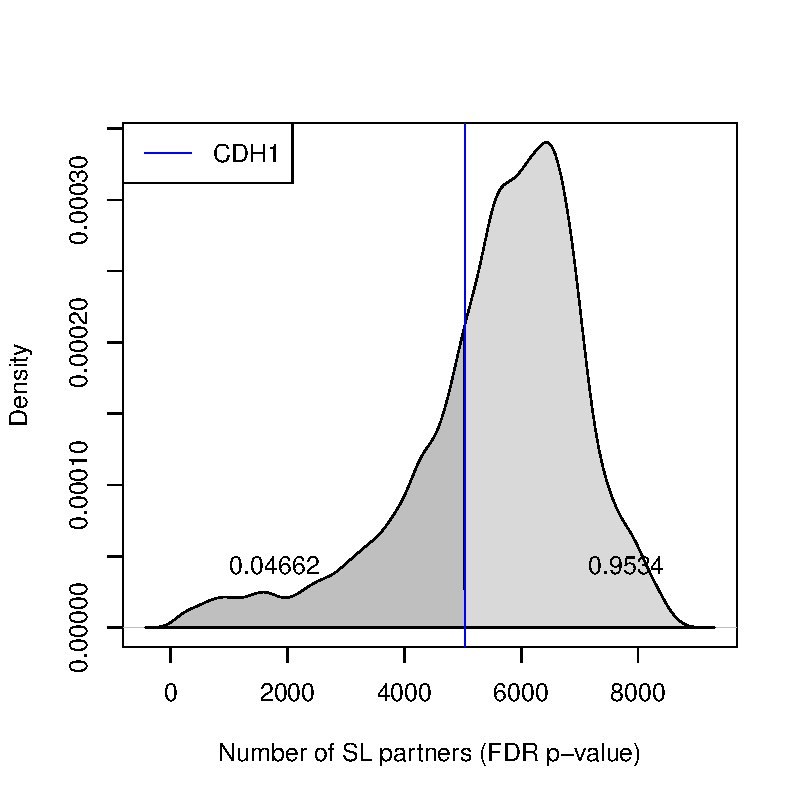
\includegraphics{MostSL_Summary_CDH1_FDR.pdf}
   }
   \end{center}
   \caption[Synthetic lethal partners across query genes]{\small \textbf{Synthetic lethal partners across query genes.} Global \gls{synthetic lethal} pairs were examined across the \glspl{genome} in \gls{TCGA} breast \glslink{gene expression}{expression} data by applying \gls{SLIPT} across query genes. The high number of predicted partners for \textit{CDH1} was typical for a human gene and lower than many other genes.
   }
\label{fig:global_SL}
%\end{mdframed}
\end{figure*}

The number of detected candidates reported here is higher than in Figures~\ref{fig:Venn_allgenes} and~\ref{fig:Venn_allgenes_stad} because these exlcuded genes not tested by the \gls{siRNA} primary screen \citep{Telford2015} for comparison with it. For an statistically rigorous measure of global \glspl{synthetic lethal}, multiple comparison procedures would need to be performed for all pairs of genes tested. However, only partner genes for each query \gls{SLIPT} analysis were performed for the purposes of comparing the number of partners predicted with those observed for \textit{CDH1} throughout this thesis.


\FloatBarrier

\subsection{Hub Genes}

The genes with the most \gls{synthetic lethal} interactions by this \gls{SLIPT} analysis are the ``hub'' genes of a \gls{synthetic lethal} network. These genes with the highest number of candidate partners detected by \gls{SLIPT} in \gls{TCGA} breast cancer \glslink{gene expression}{expression} data are summarised in Table~\ref{tab:gene_mostSL}.  These include several genes involved in cellular signalling such as \textit{TGFBR2}, \textit{PDGFRA}, \textit{FAM126A}, \textit{KCTD12}, \textit{MAML2}, and \textit{CAV1}. Gene regulation including chromatin, \acrshort{DNA}, and \acrshort{RNA} bindings genes were also observed as hub genes such as \textit{CELF2}, \textit{PLAGL1}, \textit{TSHZ2}, \textit{FOXO1}, and \textit{SVEP1}. Genes involved in the cellular membrane such as \textit{ANXA1} and \textit{FAM171A1} were also observed in addition to genes specifically implicated in cell adhesion and tight junctions such as \textit{TNS1}, \textit{BOC}, \textit{AMOTL1}, \textit{FAT4}, and \textit{EPB41L2}.

\begin{table*}[!ht]
\caption{Query \gls{synthetic lethal} genes with the most SLIPT partners}
\label{tab:gene_mostSL}
\centering
\resizebox{0.8 \textwidth}{!}{
\begin{threeparttable}
\begin{tabular}{>{\em}sl^c^c^c^c^c}
\rowstyle{\bfseries}
  \em{Gene} & Direction & raw p-value & p-value (\gls{FDR}) & \gls{SLIPT} raw p-value & \gls{SLIPT} (\gls{FDR}) \\ 
  \hline
  \rowcolor{black!10}
  TGFBR2 & 8134 & 17982 & 17973 & 8007 & 8006 \\ 
  \rowcolor{black!5}
  A2M & 8571 & 17605 & 17583 & 8345 & 8339 \\ 
  \rowcolor{black!10}
  TNS1 & 8019 & 17949 & 17934 & 7874 & 7873 \\ 
  \rowcolor{black!5}
  PROS1 & 8539 & 17668 & 17642 & 8317 & 8310 \\ 
  \rowcolor{black!10}
  ANXA1 & 9085 & 17330 & 17302 & 8689 & 8682 \\ 
  \rowcolor{black!5}
  CELF2 & 8665 & 17406 & 17368 & 8370 & 8355 \\ 
  \rowcolor{black!10}
  BOC & 8694 & 17371 & 17348 & 8384 & 8381 \\ 
  \rowcolor{black!5}
  PLAGL1 & 8792 & 17361 & 17327 & 8448 & 8436 \\ 
  \rowcolor{black!10}
  PDGFRA & 8296 & 17650 & 17621 & 8095 & 8087 \\ 
  \rowcolor{black!5}
  FAM171A1 & 8874 & 17560 & 17533 & 8567 & 8562 \\ 
  \rowcolor{black!10}
  FAM126A & 8510 & 17383 & 17356 & 8184 & 8178 \\ 
  \rowcolor{black!5}
  TSHZ2 & 7942 & 17983 & 17976 & 7787 & 7786 \\ 
  \rowcolor{black!10}
  KCTD12 & 8366 & 17651 & 17621 & 8115 & 8108 \\ 
  \rowcolor{black!5}
  MAML2 & 8336 & 17537 & 17503 & 8069 & 8061 \\ 
  \rowcolor{black!10}
  FOXO1 & 8027 & 17753 & 17737 & 7840 & 7836 \\ 
  \rowcolor{black!5}
  AMOTL1 & 8425 & 17388 & 17347 & 8147 & 8139 \\ 
  \rowcolor{black!10}
  FAT4 & 8111 & 17750 & 17732 & 7925 & 7919 \\ 
  \rowcolor{black!5}
  CAV1 & 8645 & 17491 & 17464 & 8342 & 8331 \\ 
  \rowcolor{black!10}
  SVEP1 & 7945 & 17859 & 17842 & 7791 & 7784 \\ 
  \rowcolor{black!5}
  EPB41L2 & 8415 & 17327 & 17296 & 8097 & 8092 \\ 
  \hline
\end{tabular}
\begin{tablenotes}
\raggedright \small
Genes with the most candidate \gls{synthetic lethal} partners \gls{SLIPT} in \gls{TCGA} breast \glslink{gene expression}{expression} data with the number of partner genes predicted by direction criteria and $\chi^2$ testing separately and combined as a \gls{SLIPT} analysis. Where specified, the p-values for the $\chi^2$ test were adjusted for multiple tests (\gls{FDR}).
\end{tablenotes}
\end{threeparttable}
}
\end{table*}

Genes involved in adhesion and tight junctions were also hub genes in stomach cancer (shown in Table~\ref{tab:gene_mostSL_stad}) such as \textit{HEG1}, \textit{FAT4}, \textit{NFASC}, \textit{LAMA4}, \textit{LAMC1}, \textit{TNS1}, and \textit{AMOTL1}. These also included cytoskeletal genes such as \textit{ANK2}, \textit{TTC28}, and \textit{MACF1}. Cancer genes were also among hub genes across breast and stomach cancer such as \textit{BOC}, \textit{FAT4}, and \textit{MRVI1}. 

It is therefore unsurprising that signalling and regulatory genes have been detected throughout this thesis. Not only are they suitable targets for anti-cancer therapy, they are also highly interacting genes themselves and so it is plausible that their interactions would be detectable by \gls{SLIPT}. This is consistent with the established role of abberant signalling and gene regulation in proliferation and survival of tumours and the importance of these pathways in development with highly redundant functions across many genes under complex regulation. These are also highly amenable to detection by \gls{SLIPT} analysis of \glslink{gene expression}{expression} data since their functions are dynamically regulated with corresponding changes in \glslink{gene expression}{expression}.

Cytoskeletal, membrane bound, and extracellular matrix genes are also among highly interacting \gls{synthetic lethal} hubs, including focal adhesion, tight junctions, microtubules, and fibronectin. These support the use of \gls{synthetic lethal} interactions to target \textit{CDH1}, as a \gls{tumour suppressor} gene involved in these functions. Cellular structure and cell-cell interactions are thus important functions with highly redundant genes for which there are many feasible \gls{synthetic lethal} interactions by which to understand regulation of cellular functions. These functions may also be exploited as vulnerabilities in cancer as they are frequently disruped in cancers, including \gls{HDGC} where loss of \textit{CDH1} is a \glslink{driver mutation}{driver} of cancer proliferation and malignancy.  


\FloatBarrier

\subsection{Hub Pathways}

Pathways over-represented among \gls{TCGA} breast cancer hub genes (as shown in Table~\ref{tab:pathway_mostSL}) particularly support the importance of signalling pathways, such as the PI3K/AKT pathway, as \gls{synthetic lethal} hubs. The highly redundant natures of cell-cell interaction and the extracellular matrix functions was also further supported.


\begin{table*}[!ht]
\caption{Pathways for genes with the most SLIPT partners}
\label{tab:pathway_mostSL}
\centering
\resizebox{1 \textwidth}{!}{
\begin{threeparttable}
\begin{tabular}{lcccc}
  \cellcolor{white} \textbf{Pathways Over-represented} & \textbf{Pathway Size} & \textbf{SL Genes} & \textbf{p-value} & \textbf{p-value (\gls{FDR})} \\
  \hline
  \rowcolor{black!10}
  Constitutive Signalling by Aberrant PI3K in Cancer &  56 &  10 & $8.4 \times 10^{-16}$ & $8.7 \times 10^{-13}$ \\ 
  \rowcolor{black!5}
  PI3K/AKT Signalling in Cancer &  78 &  11 & $2.1 \times 10^{-14}$ & $1.1 \times 10^{-11}$ \\ 
  \rowcolor{black!10}
  Role of LAT2/NTAL/LAB on calcium mobilization &  96 &  12 & $7.7 \times 10^{-14}$ & $2.2 \times 10^{-11}$ \\ 
  \rowcolor{black!5}
  Complement cascade &  33 &   7 & $1.2 \times 10^{-13}$ & $2.2 \times 10^{-11}$ \\ 
  \rowcolor{black!10}
  Cell surface interactions at the vascular wall &  99 &  12 & $1.6 \times 10^{-13}$ & $2.2 \times 10^{-11}$ \\ 
  \rowcolor{black!5}
  PI3K events in ERBB4 signalling &  87 &  11 & $2.6 \times 10^{-13}$ & $2.2 \times 10^{-11}$ \\ 
  \rowcolor{black!10}
  PIP3 activates AKT signalling &  87 &  11 & $2.6 \times 10^{-13}$ & $2.2 \times 10^{-11}$ \\ 
  \rowcolor{black!5}
  PI3K events in ERBB2 signalling &  87 &  11 & $2.6 \times 10^{-13}$ & $2.2 \times 10^{-11}$ \\ 
  \rowcolor{black!10}
  PI-3K cascade:FGFR1 &  87 &  11 & $2.6 \times 10^{-13}$ & $2.2 \times 10^{-11}$ \\ 
  \rowcolor{black!5}
  PI-3K cascade:FGFR2 &  87 &  11 & $2.6 \times 10^{-13}$ & $2.2 \times 10^{-11}$ \\ 
  \rowcolor{black!10}
  PI-3K cascade:FGFR3 &  87 &  11 & $2.6 \times 10^{-13}$ & $2.2 \times 10^{-11}$ \\ 
  \rowcolor{black!5}
  PI-3K cascade:FGFR4 &  87 &  11 & $2.6 \times 10^{-13}$ & $2.2 \times 10^{-11}$ \\ 
  \rowcolor{black!10}
  Extracellular matrix organization & 238 &  22 & $4.7 \times 10^{-13}$ & $3.6 \times 10^{-11}$ \\ 
  \rowcolor{black!5}
  Muscle contraction &  62 &   9 & $4.9 \times 10^{-13}$ & $3.6 \times 10^{-11}$ \\ 
  \rowcolor{black!10}
  PI3K/AKT activation &  90 &  11 & $5.5 \times 10^{-13}$ & $3.8 \times 10^{-11}$ \\ 
  \rowcolor{black!5}
  GAB1 signalosome &  91 &  11 & $7.1 \times 10^{-13}$ & $4.6 \times 10^{-11}$ \\ 
  \rowcolor{black!10}
  Smooth Muscle Contraction &  28 &   6 & $2.4 \times 10^{-12}$ & $1.5 \times 10^{-10}$ \\ 
  \rowcolor{black!5}
  Response to elevated platelet cytosolic Ca$^{2+}$ &  82 &  10 & $2.6 \times 10^{-12}$ & $1.5 \times 10^{-10}$ \\ 
  \rowcolor{black!10}
  Signalling by SCF-KIT & 126 &  13 & $3.0 \times 10^{-12}$ & $1.6 \times 10^{-10}$ \\ 
  \rowcolor{black!5}
  Signalling by FGFR & 143 &  14 & $5.0 \times 10^{-12}$ & $2.2 \times 10^{-10}$ \\ 
   \hline
\end{tabular}
\begin{tablenotes}
\raggedright \small
Gene set over-representation analysis (hypergeometric test) for Reactome pathways in the top 500 ``hub'' genes with the most candidate \gls{synthetic lethal} partners by \gls{SLIPT} analysis of \gls{TCGA} breast \glslink{gene expression}{expression} data.
\end{tablenotes}
\end{threeparttable}
}
\end{table*}

Pathway over-representation for \gls{synthetic lethal} hub genes was replicated in \gls{TCGA} stomach cancer \glslink{gene expression}{expression} data. However, these pathways differ considerably from breast cancer, as shown in Table~\ref{tab:pathway_mostSL_stad}. Cell-cell interactions and extracellular matrix pathways, including elastic fibres, were also among the hub genes for stomach cancer. The signalling pathways differ as expected in a different tissue type, although BMP and PAK signalling were detected as hub gene functions.
\fi

\FloatBarrier

\iffalse
\section{Replication in the Cancer Cell Line Encyclopaedia} \label{chapt3:CCLE}

\FloatBarrier

\begin{table*}[!b]
\caption{Pathways for \textit{CDH1} partners from SLIPT in CCLE}
\label{tab:pathway_ccle_exprSL}
\centering
\resizebox{1 \textwidth}{!}{
\begin{threeparttable}
\begin{tabular}{lccc}
  \hline
  \cellcolor{white} \textbf{Pathways Over-represented} & \textbf{Pathway Size} & \textbf{SL Genes} & \textbf{p-value (\gls{FDR})} \\
  \hline
  \rowcolor{black!10}
  Cell Cycle & 442 & 207 & $1.2 \times 10^{-215}$ \\ 
  \rowcolor{black!5}
  Cell Cycle, Mitotic & 365 & 180 & $2.9 \times 10^{-209}$ \\ 
  \rowcolor{black!10}
  Signalling by Rho GTPases & 311 & 136 & $9.4 \times 10^{-156}$ \\ 
  \rowcolor{black!5}
  M Phase & 212 & 104 & $8.8 \times 10^{-145}$ \\ 
  \rowcolor{black!10}
  Infectious disease & 289 & 123 & $1.3 \times 10^{-142}$ \\ 
  \rowcolor{black!5}
  RHO GTPase Effectors & 207 &  98 & $5.3 \times 10^{-135}$ \\ 
  \rowcolor{black!10}
  HIV Infection & 200 &  94 & $2 \times 10^{-130}$ \\ 
  \rowcolor{black!5}
  Separation of Sister Chromatids & 140 &  77 & $5.6 \times 10^{-128}$ \\ 
  \rowcolor{black!10}
  Organelle biogenesis and maintenance & 258 & 107 & $1.4 \times 10^{-127}$ \\ 
  \rowcolor{black!5}
  Chromatin modifying enzymes & 181 &  87 & $4.7 \times 10^{-126}$ \\ 
  \rowcolor{black!10}
  Chromatin organization & 181 &  87 & $4.7 \times 10^{-126}$ \\ 
  \rowcolor{black!5}
  Mitotic Metaphase and Anaphase & 149 &  78 & $1.2 \times 10^{-124}$ \\ 
  \rowcolor{black!10}
  Mitotic Anaphase & 148 &  77 & $6.3 \times 10^{-123}$ \\ 
  \rowcolor{black!5}
  Developmental Biology & 421 & 142 & $1.6 \times 10^{-121}$ \\ 
  \rowcolor{black!10}
  RHO GTPases Activate Formins &  94 &  60 & $5.3 \times 10^{-118}$ \\ 
  \rowcolor{black!5}
  Mitotic Prometaphase &  93 &  59 & $5.4 \times 10^{-116}$ \\ 
  \rowcolor{black!10}
  Hemostasis & 421 & 138 & $7.2 \times 10^{-116}$ \\ 
  \rowcolor{black!5}
  Adaptive Immune System & 397 & 132 & $3.2 \times 10^{-115}$ \\ 
  \rowcolor{black!10}
  Assembly of the primary cilium & 143 &  72 & $2.4 \times 10^{-114}$ \\ 
  \rowcolor{black!5}
  Transcription & 133 &  68 & $6.2 \times 10^{-111}$ \\ 
   \hline
\end{tabular}
\begin{tablenotes}
\raggedright \small
Gene set over-representation analysis (hypergeometric test) for Reactome pathways in \gls{SLIPT} partners for \textit{CDH1}.
\end{tablenotes}
\end{threeparttable}
}
\end{table*}

As breast cancer cell lines are the experimental system in which many cancer genetics and drug targets are investigated, these were analysed in addition to patient samples from \gls{TCGA}. The \gls{CCLE} is a resource for \glspl{genomic} profiles across a range of cell lines. These have also been used to generate \gls{synthetic lethal} candidates for comparison to those in experimental screen and predictions from \gls{TCGA} \glslink{gene expression}{expression} data.

The cancer cell line encyclopaedia provides further support for \gls{synthetic lethal} genes and pathways that may be applicable across cell types and reproducible in experimental systems. In contrast to the homogeneous pooled cell samples of patients,  the cell lines provide a genetically homogeneous cell population in which to examine molecular functions and as a preclinical model of cancerous disease. The complete set of 1037 cell lines was tested for \glspl{synthetic lethal} across tissues, in addition to the 59 breast cell lines and 38 stomach cell lines being tested separately for partners of \textit{CDH1}. \Gls{synthetic lethal} genes were detected by \gls{SLIPT} (as described in Section~\ref{methods:SLIPT}) and over-represented \gls{synthetic lethal} Reactome pathways (as described in Section~\ref{methods:enrichment}). 

Synthetic lethal gene candidates were detectable by \gls{SLIPT} across each of these sample sets of cells lines (as shown in Tables~\ref{tab:gene_ccle_SL}\nobreakdash--\ref{tab:gene_ccle_stad_SL}. However, these were most highly significant across the samples in the \gls{CCLE} \glslink{gene expression}{expression} dataset (as shown in Table~\ref{tab:gene_ccle_SL}) and included genes detected in prior analyses such as \textit{VIM}, \textit{ZEB2}, \textit{EMP3}. Pathways were also highly over-represented among \gls{synthetic lethal} candidates for the full \gls{CCLE} dataset (as shown in Table~\ref{tab:pathway_ccle_exprSL}) including Rho GTPase (\glspl{GPCR}), immmune, and gene regulation (chromatin and transcription). This is unexpected since immune pathways would not be expected to be detectable in isolated cell lines, although this could be attributed to cytokine and integrin signalling occuring the cancer cells in addition to interactions with immune cells in the tumour microenvironment (which could not be distinguished in patient samples). Cell cycle and mitosis were among the highest \gls{synthetic lethal} pathways across cell lines supporting \textit{CDH1} deficient cells having abberant cell signalling and consequences for proliferation such as cancer cells. However, cell cycle genes were not as strongly supported in \gls{TCGA} patient samples or the \gls{siRNA} screen \citep{Telford2015} and they may not be applicable to epithelial tissues such as breast or stomach cancer or amenable to selective inhibition in experimental models.   

\begin{table*}[!tb]
\caption{Pathways for \textit{CDH1} partners from SLIPT in breast CCLE}
\label{tab:pathway_ccle_brca_exprSL}
\centering
\resizebox{1 \textwidth}{!}{
\begin{threeparttable}
\begin{tabular}{lccc}
  \hline
  \cellcolor{white} \textbf{Pathways Over-represented} & \textbf{Pathway Size} & \textbf{SL Genes} & \textbf{p-value (\gls{FDR})} \\
  \hline
  \rowcolor{black!10}
  Cell junction organization &  71 &   5 & 0.006 \\ 
  \rowcolor{black!5}
  Adherens junctions interactions &  29 &   3 & 0.006 \\ 
  \rowcolor{black!10}
  Dermatan sulfate biosynthesis &  11 &   2 & 0.006 \\ 
  \rowcolor{black!5}
  Non-integrin membrane-ECM interactions &  52 &   4 & 0.006 \\ 
  \rowcolor{black!10}
  Regulation of pyruvate dehydrogenase (PDH) complex &  12 &   2 & 0.0069 \\ 
  \rowcolor{black!5}
  Cell-extracellular matrix interactions &  17 &   2 & 0.021 \\ 
  \rowcolor{black!10}
  Pyruvate metabolism &  17 &   2 & 0.021 \\ 
  \rowcolor{black!5}
  Cell-cell junction organization &  46 &   3 & 0.039 \\ 
  \rowcolor{black!10}
  Synthesis of substrates in N-glycan biosythesis &  50 &   3 & 0.057 \\ 
  \rowcolor{black!5}
  Detoxification of Reactive Oxygen Species &  26 &   2 & 0.082 \\ 
  \rowcolor{black!10}
  Keratan sulfate biosynthesis &  28 &   2 & 0.092 \\ 
  \rowcolor{black!5}
  Laminin interactions &  28 &   2 & 0.092 \\ 
  \rowcolor{black!10}
  Cell-Cell communication & 118 &   5 & 0.12 \\ 
  \rowcolor{black!5}
  Keratan sulfate/keratin metabolism &  32 &   2 & 0.12 \\ 
  \rowcolor{black!10}
  Opioid Signalling &  63 &   3 & 0.12 \\ 
  \rowcolor{black!5}
   \begin{tabular}[c]{@{}l@{}}Biosynthesis of the N-glycan precursor (dolichol lipid-linked oligosaccharide) \\ and transfer to a nascent protein \end{tabular} &  63 &   3 & 0.12 \\ 
  \rowcolor{black!10}
  Intraflagellar transport &  34 &   2 & 0.14 \\ 
  \rowcolor{black!5}
  Signalling by Retinoic Acid &  36 &   2 & 0.16 \\ 
  \rowcolor{black!10}
  Pyruvate metabolism and Citric Acid (TCA) cycle &  36 &   2 & 0.16 \\ 
  \rowcolor{black!5}
  Nef mediated downregulation of MHC class I complex cell surface \glslink{gene expression}{expression} &  10 &   1 & 0.22 \\ 
  \hline
\end{tabular}
\begin{tablenotes}
\raggedright \small
Gene set over-representation analysis (hypergeometric test) for Reactome pathways in \gls{SLIPT} partners for \textit{CDH1}.
\end{tablenotes}
\end{threeparttable}
}
\end{table*}


Synthetic lethal pathways specific to \gls{SLIPT} candidates from breast cell lines (as shown in Table~\ref{tab:pathway_ccle_brca_exprSL}) were more consistent with previous obervations, particularly the established role of \gls{E-cadherin} in cell junctions and the Adherens complex. However, the number of \gls{SLIPT} candidate genes detected in stomach cell lines was insufficient to replicate the findings in breast cell lines to \gls{TCGA} patient samples. However, \gls{SLIPT} candidates across breast and stomach \gls{CCLE} cell lines were over-represented (as shown in Table~\ref{tab:pathway_ccle_breast_stad_exprSL}) for similar pathways to breast cell lines with additional support for extracellular matrix pathways including elastic fibres which were replicated with resampling across breast and stomach \gls{TCGA} analyses and the primary \gls{siRNA} screen \citet{Telford2015}
\fi

\FloatBarrier

\section{Discussion}

\subsection{Strengths of the SLIPT Methodology}

Synthetic lethal discovery  with \gls{SLIPT} used established statistical procedures to identify putative partner genes from \gls{gene expression} data. Such use of the $\chi^2$-value is amenable to pathway or permutation analyses and could feasibly be applied to other disease gene or pair-wise across the \glspl{genome}, although \glspl{genome}-wide approaches were unable to find informative candidate genes for \gls{E-cadherin} \citep{Lu2015}. \Gls{synthetic lethal} discovery in cancer has focused on genes with severe cellular \gls{mutant} phenotypes, such as \gls{essential} genes or the \glspl{oncogene} \textit{TP53} and \textit{AKT} \citep{Tiong2014, Lu2015, Wang2013}, with other cancer genes, such as \textit{CDH1}, requiring more focused investigations. Prior computational approaches for \gls{synthetic lethal} discovery, in cancer, vary widely \citep{Tiong2014, Jerby2014, Lu2015, Wappett2016}. There is no consensus as to which approach is more appropriate, and the methods are difficult to compare, as they either do not have a released code implementation or do not make predictions solely from normalised \glslink{gene expression}{expression} data.

However, the query-based approach demonstrated by \gls{SLIPT} analysis is suitable for wider application on \glslink{gene expression}{expression} data and for augmenting experimental studies such as high-throughput screens. This approach has identified biologically plausible \gls{synthetic lethal} pathways for \textit{CDH1}, triaged candidates from experimental screening \citep{Telford2015}, and replicates genes and pathways across breast and stomach cancer datasets. In addition, \gls{SLIPT} avoids critical assumptions underlying the design of some approaches such as co-expression of synthetic candidates or that interacting gene pairs will have known (annotated) similarities in function.

The DAISY methodology \cite{Jerby2014}, which took a similar query-based approach with the \gls{tumour suppressor} \textit{VHL}, has been critiqued for being too stringent \citep{Lu2015} which impedes pathway analysis. Since \gls{functional redundancy} does not require genes to be expressed at the same time, the \gls{SLIPT} approach does not assume co-expression of \gls{synthetic lethal} genes which may enrich for \gls{synthetic lethal} genes in established coregulated pathways. Rather, the interpretation of \glspl{synthetic lethal} for \gls{SLIPT} was similar to other computational methods based on `co-loss under-represent\-at\-ion', `compensation', or `simultaneous differential \glslink{gene expression}{expression}' \citep{Tiong2014, Lu2015, Wang2013}.

Genomics analyses are prone to false-positives and require statistical caution, particularly where working with gene-pairs scale sup the number of multiple tests drastically, at the expense of statistical power.  Experimental screens for \glspl{synthetic lethal} are also error-prone \citep{Lu2015, Fece2015, Lord2014}, especially with false-positives, raising the need for understanding the expected behaviour and number of functional relationships and genetic interactions in the \glspl{genome}, or in discovery of \gls{synthetic lethal} partners of a particular query gene. Thus analyses throughout this thesis have focused on querying for partners of a particular gene of interest. Statistical modelling and simulations (in Section~\ref{chapt2:simulation_2015} and Chapter~\ref{chap:simulation}) will further support the design decisions underlying \gls{SLIPT} analysis and its strengths over other approaches.

\subsection{Synthetic Lethal Pathways for \gls{E-cadherin}}

Specific genes were difficult to replicate across experiments. This is consistent with \gls{gene expression} profiles for \gls{synthetic lethal} partners reflecting the complexity of biological pathways which are subject to higher-order interactions and do not consistently compensate for loss of gene function across all samples \citep{Kelly2013, Jerby2014, Lu2015}. The predicted \gls{synthetic lethal} partners of \textit{CDH1} (with \gls{FDR} correction) were investigated with \gls{gene expression} profiles and clinical variables to find relationships in \gls{gene expression}, gene function, and clinical characteristics. The large number of genes detected indicates that \gls{synthetic lethal} detection is potentially error-prone, and that identifying genes relevant for clinical application will be difficult without a supporting biological pathway rationale. As such, investigations into the genes identified by \gls{SLIPT}, the correlation structure between them, and those which were validated by experimental screening \citep{Telford2015} focused at the pathway level throughout this Chapter. Similarly, comparisons across analyses were largely made at the pathway level, including comparisons between \glslink{gene expression}{expression} and \gls{mutation}, breast and stomach \gls{TCGA} datasets.%, and patient sample data with cell line \glslink{gene expression}{expression} profiles.

Potential \gls{synthetic lethal} partners of \textit{CDH1} identified by \gls{SLIPT} had many distinct functions, with each gene cluster highly expressed in different patient subgroups (Figure~\ref{fig:slipt_expr}). The \glslink{gene expression}{expression} profiles of the SL partners of \textit{CDH1} predicted from \gls{TCGA} breast cancer \gls{RNA-Seq} data (expected to have compensating high or stable \glslink{gene expression}{expression}) and their corresponding functional enrichment found  in subgroups of genes, particularly among \textit{CDH1} low breast tumours.  Ductal breast cancers showed higher \glslink{gene expression}{expression} of \gls{synthetic lethal} partners suggesting treatment would be more effective in this tumour subtype.  However, there was consistently low \glslink{gene expression}{expression} of SL partners in estrogen receptor negative tumours, although this is independent of tumour stage and consistent with poor prognosis in these patients and could inform other treatment strategies or prevent ineffective treatment further impacting quality of life in these patients.  These results suggest that \gls{synthetic lethal} partner \glslink{gene expression}{expression} varies between patients; that these different tumour classes would react differently to the same treatment; that treatment of different pathways and combinations in different patients is the most effective approach to target genes compensating for \textit{CDH1} gene loss; and that the \glslink{gene expression}{expression} of synthetic partners could be a clinically important biomarker.  

The pathways that \gls{synthetic lethal} partners of \textit{CDH1} identified by \gls{SLIPT} were involved in a diverse range of biological functions and differed to those detected experimentally. This discrepancy may be accounted for by \gls{gene expression} analyses detecting both \gls{synthetic lethal} partners, as screened for experimentally by \citet{Telford2015}, and their downstream targets (not detected by \gls{siRNA}), capturing the wider pathways and mechanisms involved in \glspl{synthetic lethal} with \textit{CDH1} inactivation. In particular, \gls{GPCR} phosphorylation cascades (which regulate \gls{gene expression} and translation in cancers \citep{Gao2015}) were predicted to be \gls{synthetic lethal} with \textit{CDH1}. The predicted \gls{synthetic lethal} partners occurred across functionally distinct pathways, including characterised functions of \textit{CDH1}. The most consistently supported pathways included elastic fibres in the extracelullar matrix, \gls{GPCR} signalling, and translation presenting vulnerabilities for \textit{CDH1} deficient cancer cells from extracellular stimuli to the core growth mechanisms of a cell.

This diversity in \gls{synthetic lethal} functions is consistent with the wide ranging role of \textit{CDH1} in cell-cell adhesion, cell signalling, and the cytoskeletal structure of epithelial tissues. Pathway structure may be relevant to identifying potential drug targets from \gls{gene expression} signatures, indicating downstream effector genes and mechanisms leading to cell inviability. Identification of distinct \gls{synthetic lethal} gene clusters may further lead to the elucidation of drug resistance mechanisms. While these pathways are indicative of the main functions of \gls{E-cadherin} and \gls{synthetic lethal} partners, it remains to identify the genes within these pathways that are the most actionable or supported across \gls{SLIPT} analysis in patient samples and detected by experiments in preclinical models \citep{Chen2014, Telford2015}.  The specific genes within key pathways will be be discussed in Chapter~\ref{chap:Pathways}, along with further investigations into their relation to \glslink{graph}{pathway} structure.  While these are important clinical implications, the \gls{synthetic lethal} predictions lack enough confidence for direct translation into pre-clinical models or clinical applications leading to a need for statistical modelling and simulation of \glspl{synthetic lethal} in \glspl{genomic} \glslink{gene expression}{expression} data.

These \gls{synthetic lethal} pathways have potential clinical implications, particularly those supported in pre-clinical models and in patient \glslink{gene expression}{expression} data. However, further validation of gene candidates will be necessary to ensure that these are able to reproduced in further pre-clinical studies, they are applicable to tumours \textit{in vivo}, and that effective inhibitory agents can be repurposed or designed against them.

\subsection{Replication and Validation}

\subsubsection{Integration with \gls{siRNA} Screening}

The pathway composition across computational and experimental \gls{synthetic lethal} candidates was informative with over-represent\-ation (Table~\ref{tab:Venn_over-representation}) and supported by resampling analysis (Table~\ref{tab:pathway_perm_overlap}), despite a modest intersection of genes between them (Figure~\ref{fig:Venn_allgenes}). Either approach may be significant for a pathway in this intersection without being supported by the other: resampling analysis may support pathways that were not over-represent\-ed due to small effect sizes, thus both tests are required for a candidate pathway.

The pathways detected by both over-represent\-ation and resampling are the strongest candidates for further investigation and the \glslink{graph}{pathway} structure analyses in Chapter~\ref{chap:Pathways} will focus on these pathways detected by both over-representation and resampling. Particularly, those replicated across datasets or with pathway \glspl{metagene}. In addition to GCPR pathways detected across these analyses, the \gls{PI3K} cascade will also be investigated in Chapter~\ref{chap:Pathways}, this signalling pathway is a well characterised mediator between GCPR receptors and regulation of translation \citep{Gao2015} (both detected throughout this Chapter) and exhibited unexpected behaviour with pathway the \glspl{metagene} (in Section~\ref{chapt3:metagene_results}). This pathway is activated by protein Phosphorylation states and thus inactivatino may not be detectable with \glslink{gene expression}{expression}.

However, the \gls{SLIPT} approach was shown to be predictive of which \gls{siRNA} primary screen candidate partners of \textit{CDH1} were validated in a secondary screen (as shown in Section~\ref{chapt3:secondary_screen}). These results further support \gls{SLIPT} for identifying robust \gls{synthetic lethal} candidates which can be validated and as a triage approach for interpreting screening experiments.

\subsubsection{Replication across Tissues}

Furthermore, \gls{synthetic lethal} partners identified by \gls{SLIPT} were replicated across breast and stomach cancer. These were particularly concordant at the pathway level, as expected between tissues since \gls{synthetic lethal} pathways have higher conservation between species \citep{Dixon2008}. These findings support gene functions conserved across \textit{CDH1} deficient cancers in breast and stomach tissues, presenting vulnerabilities that could be applied against molecular targets in both cancers. In addition, these analyses serve as a replication across independent patient cohorts from breast and stomach cancers, decreasing the likelihood of the \gls{synthetic lethal} pathways detected being false positives or artifacts of either dataset.

Synthetic lethal pathways were also replicated across \glslink{gene expression}{expression} analyses of \gls{TCGA} patient samples in heterogeneous tumours and homogeneous cell line isolates. This further supports that the subset of \gls{synthetic lethal} functions detectable in experimental models \citep{Chen2014, Telford2015} would be applicable tumours of patients with \textit{CDH1} deficient cancers.

There are many gene functions replicated across breast cancer \gls{gene expression} analyses. Many of these were also replicated with \gls{mutation} analysis and with stomach cancer or cell line \glslink{gene expression}{expression} data. These pathways were more consistent across replication analyses than previous investigations with \gls{TCGA} \gls{microarray} data \citep{Kelly2013}.   

\section{Summary}

We have developed a simple, interpretable, computational approach to predict \gls{synthetic lethal} partners from \glspl{genomic} data. The analyses focus on \gls{gene expression} data as it is widely available for applications in other cancers and other disease genes, particularly those with malignant loss of function.

This approach has been applied to robustly detect \gls{synthetic lethal} pathways for the \gls{E-cadherin} (\textit{CDH1}) in \gls{TCGA} breast cancer molecular profiles with comparisons to experimental screening \citep{Telford2015} in cell lines, and replication in \gls{TCGA} stomach cancer molecular profiles and across cell types in the cancer cell line encyclopaedia. The pathway replicated across several analyses included extracellular matrix pathways (e.g., elastic fibres formation), cell signalling (including \glspl{GPCR}), and core gene regulation and translation processes crucial for the growth and proliferation of cancer cells. These pathways show evidence of \gls{non-oncogene addiction} for \textit{CDH1} deficient cells and present vulnerabilities which may be exploited for specific treatment against \textit{CDH1} \glspl{mutation} in HCGC and \glslink{sporadic}{sporadic} cancers. There was also support for \gls{synthetic lethal} pathways with \textit{CDH1} in cell adhesion and cytoskeletal processes to which \textit{CDH1} belongs, supporting the finding that \glspl{synthetic lethal} occurs within biological pathways \citep{Kelley2005, Boone2007}.

While translational and immune pathways detected by \gls{SLIPT} were not supported by primary \gls{siRNA} screening \citep{Telford2015}, these were replicated across various analyses. Due to the differences between an experimental cell line model \citep{, Chen2014, Fece2015}%Barretina2012
and patient molecular profiles \citep{TCGA2012, TCGA2014GC}, these would not be expected to be completely concordant. Furthermore, many pathways are difficult to test in an isolated experimental system. Nevertheless, many of the genes and pathways detected by \gls{SLIPT} are suitable to inform further investigations and triage of therapeutic targets against \textit{CDH1} deficient tumours in combination with experimental screening.  

A characteristic of gene interaction networks is a \gls{scale-free} topology leading to highly interacting ‘hub’ genes, these represent important genes in a functional network. Cell surface interactions, the extracellular matrix, and cell signalling (particularly PI3K/AKT signalling) were also found to be \gls{synthetic lethal} hubs with more interactions detected than other genes. This indicates that these pathways are functionally important to survival of cancer cells since they are subject to high \gls{functional redundancy}, despite frequent disruptions in cancer. These pathways being involved in a disproportionate number of \gls{synthetic lethal} interactions is also consistent with their detection for \textit{CDH1}.

Thus \gls{synthetic lethal} pathways have been identified using \gls{TCGA} patient molecular profiles%, \gls{CCLE} cancer cell line \glslink{gene expression}{expression} data,
and experimental screening results. Some these were robustly replicated across these datasets and against \textit{CDH1} \gls{mutation} or \glslink{gene expression}{expression} analysis. However, there remains the need to identify actionable genes within these pathways, relationships with experimental candidates, and how these pathways may affect viability when lost. While the genes identified between these analyses were less concordant the results of the \gls{TCGA} breast cancer analysis will be used to test \glslink{graph}{pathway} structure relationships and further examine the \gls{synthetic lethal} genes detected in the following Chapter.

%%from chapter intro
%Together these results demonstrate the wide range of applications for \gls{SLIPT} analysis and examine the \gls{synthetic lethal} partners of \textit{CDH1} in breast and stomach cancer. These \gls{synthetic lethal} genes and pathways were identified both in the context of the functional implications of novel \gls{synthetic lethal} relationships and as potential actionable targets against \textit{CDH1} deficient tumours, in addition to replication of established functions of \gls{E-cadherin}. In particular, these analyses focused on comparisons with experimental screening data to explore the potential for \gls{SLIPT} to augment triage of candidate partners and support further experimental investigations. The key \gls{synthetic lethal} partner pathways for \textit{CDH1}, supported by both approaches, will be examined in more detail at the gene and \glslink{graph}{pathway} structure level in Chapter~\ref{chap:Pathways}.

\clearpage

\iffalse

\paragraph{Aims}

  \begin{itemize}
   \item Pathway Structure of Candidate Synthetic Lethal Genes for \textit{\textit{CDH1}} from \gls{TCGA} breast data
   
   \bigskip
   
   \item Comparisons to Experimental \gls{siRNA} Screen Candidates
   
   \bigskip
   
   \item Replication of Pathways across in \gls{TCGA} Stomach data
  \end{itemize}

\paragraph{Summary}

    
  \begin{itemize}
   \item We have developed a Synthetic Lethal detection method that generates a high number of \gls{synthetic lethal} candidates
   
   \bigskip
   
   \item Pathways in cell signalling, extracellular matrix, and cytoskeletal functions were supported with experimental candidates and the known functions of \gls{E-cadherin}
   
   \bigskip
   
   \item Several candidate pathways were supported by \gls{mutation} analysis and replicated across breast and stomach cancer
   
   \bigskip
   
   \item Translation and immune functions were uniquely detected by the computational approach which may be explained by differences between patient samples and cell line models
   
   \bigskip
   
   \item There remains the need to identify actionable genes within these pathways, relationships with experimental candidates, and how these pathways may affect viability when lost
  \end{itemize}
  \fi